% The arXiv version of the thesis_revised report, in the ICLR conference style (iclr2027_conference.sty,
% with the running header patched from "Published as a conference paper at ICLR 2027" to "Preprint").
% Every number is a \V{key} read from generated/*.tex; the tables and figures come from
% make_arxiv_assets.py, which takes them from the thesis's own generators with each design named in
% words. Build from src/probes/deception-detection:
%   python paper/arxiv/make_arxiv_assets.py
%   cd arxiv && tectonic main.tex --keep-logs --keep-intermediates
\documentclass{article}
\usepackage[T1]{fontenc}
\usepackage{iclr2027_conference,times}
\usepackage{amsmath,amssymb}
\usepackage{booktabs,multirow,array,tabularx}
\usepackage{graphicx}
\usepackage{tikz} % the style file has already loaded xcolor
\usetikzlibrary{arrows.meta,positioning,fit,calc,shapes.geometric}
\usepackage{enumitem}
\usepackage{placeins}
\usepackage{hyperref}
\usepackage{url}
\usepackage[capitalize,noabbrev]{cleveref}
\graphicspath{{images/}}

% Anonymity. \anonymousfalse is the arXiv preprint: the authors are shown (the style's final-copy
% switch) and the repository is named. \anonymoustrue builds the double-blind version for a
% conference submission from the same source.
\newif\ifanonymous
\anonymousfalse
\ifanonymous\else\iclrfinalcopy\fi

% Every result is read as \V{key}; an unknown key stops the build instead of printing a blank.
\makeatletter
\newcommand{\setV}[2]{\expandafter\def\csname num@#1\endcsname{#2}}
\newcommand{\V}[1]{\ifcsname num@#1\endcsname\csname num@#1\endcsname\else
  \PackageError{numbers}{Undefined number `#1'}{Run make_arxiv_assets.py}\fi}
\makeatother
% Generated by make_numbers.py -- do not edit.
\setV{n-cg}{267}
\setV{ndec-cg}{167}
\setV{n-hpc}{2,134}
\setV{ndec-hpc}{134}
\setV{n-hpkr}{2,139}
\setV{ndec-hpkr}{139}
\setV{n-it}{1,080}
\setV{ndec-it}{423}
\setV{n-id}{5,432}
\setV{ndec-id}{3,045}
\setV{n-repe}{550}
\setV{ndec-repe}{275}
\setV{n-control}{2,000}
\setV{bank-personas}{36}
\setV{bank-new}{10}
\setV{bank-kept}{3,749}
\setV{bank-generated}{5,400}
\setV{bank-kept-min}{47}
\setV{bank-kept-max}{149}
\setV{bank-kept-pct}{69}
\setV{zs-dec-cg-L20}{0.940}
\setV{zs-dec-hpc-L20}{0.717}
\setV{zs-dec-hpkr-L20}{0.148}
\setV{zs-dec-it-L20}{0.988}
\setV{zs-dec-id-L20}{0.959}
\setV{zs-dec-repe-L20}{0.994}
\setV{zs-dec-mean-L20}{0.791}
\setV{zs-dec-lb-L20}{0.750}
\setV{zs-den-cg-L20}{0.931}
\setV{zs-den-hpc-L20}{0.585}
\setV{zs-den-hpkr-L20}{0.890}
\setV{zs-den-it-L20}{0.976}
\setV{zs-den-id-L20}{0.932}
\setV{zs-den-repe-L20}{0.882}
\setV{zs-den-mean-L20}{0.866}
\setV{zs-den-lb-L20}{0.863}
\setV{zs-ext-cg-L20}{0.969}
\setV{zs-ext-hpc-L20}{0.639}
\setV{zs-ext-hpkr-L20}{0.882}
\setV{zs-ext-it-L20}{0.990}
\setV{zs-ext-id-L20}{0.954}
\setV{zs-ext-repe-L20}{0.991}
\setV{zs-ext-mean-L20}{0.904}
\setV{zs-ext-lb-L20}{0.887}
\setV{zs-syc-cg-L20}{0.999}
\setV{zs-syc-hpc-L20}{0.533}
\setV{zs-syc-hpkr-L20}{0.043}
\setV{zs-syc-it-L20}{0.983}
\setV{zs-syc-id-L20}{0.923}
\setV{zs-syc-repe-L20}{0.977}
\setV{zs-syc-mean-L20}{0.743}
\setV{zs-syc-lb-L20}{0.696}
\setV{zs-pcone-cg-L20}{0.942}
\setV{zs-pcone-hpc-L20}{0.700}
\setV{zs-pcone-hpkr-L20}{0.253}
\setV{zs-pcone-it-L20}{0.989}
\setV{zs-pcone-id-L20}{0.959}
\setV{zs-pcone-repe-L20}{0.991}
\setV{zs-pcone-mean-L20}{0.806}
\setV{zs-pcone-lb-L20}{0.769}
\setV{zs-extpcone-cg-L20}{0.737}
\setV{zs-extpcone-hpc-L20}{0.615}
\setV{zs-extpcone-hpkr-L20}{0.559}
\setV{zs-extpcone-it-L20}{0.681}
\setV{zs-extpcone-id-L20}{0.772}
\setV{zs-extpcone-repe-L20}{0.604}
\setV{zs-extpcone-mean-L20}{0.661}
\setV{zs-extpcone-lb-L20}{0.673}
\setV{zs-dec-cg-L40}{0.865}
\setV{zs-dec-hpc-L40}{0.581}
\setV{zs-dec-hpkr-L40}{0.593}
\setV{zs-dec-it-L40}{0.979}
\setV{zs-dec-id-L40}{0.974}
\setV{zs-dec-repe-L40}{1.000}
\setV{zs-dec-mean-L40}{0.832}
\setV{zs-dec-lb-L40}{0.798}
\setV{zs-den-cg-L40}{0.902}
\setV{zs-den-hpc-L40}{0.755}
\setV{zs-den-hpkr-L40}{0.919}
\setV{zs-den-it-L40}{0.913}
\setV{zs-den-id-L40}{0.980}
\setV{zs-den-repe-L40}{1.000}
\setV{zs-den-mean-L40}{0.912}
\setV{zs-den-lb-L40}{0.894}
\setV{zs-ext-cg-L40}{0.912}
\setV{zs-ext-hpc-L40}{0.712}
\setV{zs-ext-hpkr-L40}{0.912}
\setV{zs-ext-it-L40}{0.980}
\setV{zs-ext-id-L40}{0.978}
\setV{zs-ext-repe-L40}{1.000}
\setV{zs-ext-mean-L40}{0.916}
\setV{zs-ext-lb-L40}{0.899}
\setV{zs-syc-cg-L40}{0.998}
\setV{zs-syc-hpc-L40}{0.751}
\setV{zs-syc-hpkr-L40}{0.167}
\setV{zs-syc-it-L40}{0.985}
\setV{zs-syc-id-L40}{0.948}
\setV{zs-syc-repe-L40}{0.999}
\setV{zs-syc-mean-L40}{0.808}
\setV{zs-syc-lb-L40}{0.770}
\setV{zs-pcone-cg-L40}{0.906}
\setV{zs-pcone-hpc-L40}{0.599}
\setV{zs-pcone-hpkr-L40}{0.693}
\setV{zs-pcone-it-L40}{0.982}
\setV{zs-pcone-id-L40}{0.975}
\setV{zs-pcone-repe-L40}{1.000}
\setV{zs-pcone-mean-L40}{0.859}
\setV{zs-pcone-lb-L40}{0.831}
\setV{zs-extpcone-cg-L40}{0.813}
\setV{zs-extpcone-hpc-L40}{0.564}
\setV{zs-extpcone-hpkr-L40}{0.736}
\setV{zs-extpcone-it-L40}{0.546}
\setV{zs-extpcone-id-L40}{0.958}
\setV{zs-extpcone-repe-L40}{0.990}
\setV{zs-extpcone-mean-L40}{0.768}
\setV{zs-extpcone-lb-L40}{0.723}
\setV{zs-dec-cg-L44}{0.819}
\setV{zs-dec-hpc-L44}{0.607}
\setV{zs-dec-hpkr-L44}{0.589}
\setV{zs-dec-it-L44}{0.979}
\setV{zs-dec-id-L44}{0.962}
\setV{zs-dec-repe-L44}{1.000}
\setV{zs-dec-mean-L44}{0.826}
\setV{zs-dec-lb-L44}{0.791}
\setV{zs-den-cg-L44}{0.858}
\setV{zs-den-hpc-L44}{0.725}
\setV{zs-den-hpkr-L44}{0.908}
\setV{zs-den-it-L44}{0.933}
\setV{zs-den-id-L44}{0.978}
\setV{zs-den-repe-L44}{1.000}
\setV{zs-den-mean-L44}{0.900}
\setV{zs-den-lb-L44}{0.880}
\setV{zs-ext-cg-L44}{0.859}
\setV{zs-ext-hpc-L44}{0.712}
\setV{zs-ext-hpkr-L44}{0.894}
\setV{zs-ext-it-L44}{0.982}
\setV{zs-ext-id-L44}{0.974}
\setV{zs-ext-repe-L44}{1.000}
\setV{zs-ext-mean-L44}{0.903}
\setV{zs-ext-lb-L44}{0.884}
\setV{zs-syc-cg-L44}{0.983}
\setV{zs-syc-hpc-L44}{0.692}
\setV{zs-syc-hpkr-L44}{0.480}
\setV{zs-syc-it-L44}{0.987}
\setV{zs-syc-id-L44}{0.949}
\setV{zs-syc-repe-L44}{1.000}
\setV{zs-syc-mean-L44}{0.848}
\setV{zs-syc-lb-L44}{0.818}
\setV{zs-pcone-cg-L44}{0.859}
\setV{zs-pcone-hpc-L44}{0.633}
\setV{zs-pcone-hpkr-L44}{0.665}
\setV{zs-pcone-it-L44}{0.982}
\setV{zs-pcone-id-L44}{0.966}
\setV{zs-pcone-repe-L44}{1.000}
\setV{zs-pcone-mean-L44}{0.851}
\setV{zs-pcone-lb-L44}{0.821}
\setV{zs-extpcone-cg-L44}{0.784}
\setV{zs-extpcone-hpc-L44}{0.583}
\setV{zs-extpcone-hpkr-L44}{0.715}
\setV{zs-extpcone-it-L44}{0.663}
\setV{zs-extpcone-id-L44}{0.962}
\setV{zs-extpcone-repe-L44}{0.973}
\setV{zs-extpcone-mean-L44}{0.780}
\setV{zs-extpcone-lb-L44}{0.742}
\setV{off-base-L20}{0.648}
\setV{offx-base-L20}{0.728}
\setV{diag-base-L20}{0.956}
\setV{off-dec-L20}{0.651}
\setV{offx-dec-L20}{0.919}
\setV{diag-dec-L20}{0.908}
\setV{off-den-L20}{0.866}
\setV{offx-den-L20}{0.861}
\setV{diag-den-L20}{0.865}
\setV{off-ext-L20}{0.904}
\setV{offx-ext-L20}{0.909}
\setV{diag-ext-L20}{0.904}
\setV{off-pcone-L20}{0.667}
\setV{offx-pcone-L20}{0.916}
\setV{diag-pcone-L20}{0.887}
\setV{off-pcthree-L20}{0.679}
\setV{offx-pcthree-L20}{0.888}
\setV{diag-pcthree-L20}{0.919}
\setV{off-extpcone-L20}{0.661}
\setV{offx-extpcone-L20}{0.682}
\setV{diag-extpcone-L20}{0.643}
\setV{off-extpcthree-L20}{0.684}
\setV{offx-extpcthree-L20}{0.900}
\setV{diag-extpcthree-L20}{0.915}
\setV{off-denpcthree-L20}{0.710}
\setV{offx-denpcthree-L20}{0.752}
\setV{diag-denpcthree-L20}{0.875}
\setV{off-rand-L20}{0.527}
\setV{offx-rand-L20}{0.560}
\setV{diag-rand-L20}{0.787}
\setV{off-syc-L20}{0.615}
\setV{offx-syc-L20}{0.883}
\setV{diag-syc-L20}{0.892}
\setV{off-sycpcone-L20}{0.615}
\setV{offx-sycpcone-L20}{0.884}
\setV{diag-sycpcone-L20}{0.893}
\setV{off-sycthree-L20}{0.657}
\setV{offx-sycthree-L20}{0.823}
\setV{diag-sycthree-L20}{0.931}
\setV{gap-ext-base-L20}{0.256}
\setV{gap-ext-extpcthree-L20}{0.220}
\setV{gap-ext-dec-L20}{0.253}
\setV{drop-base-L20}{0.309}
\setV{pt-base-cg-L20}{0.663}
\setV{pt-base-hpc-L20}{0.535}
\setV{pt-base-hpkr-L20}{0.394}
\setV{pt-base-it-L20}{0.799}
\setV{pt-base-id-L20}{0.778}
\setV{pt-base-repe-L20}{0.718}
\setV{pt-dec-cg-L20}{0.764}
\setV{pt-dec-hpc-L20}{0.630}
\setV{pt-dec-hpkr-L20}{0.148}
\setV{pt-dec-it-L20}{0.793}
\setV{pt-dec-id-L20}{0.775}
\setV{pt-dec-repe-L20}{0.796}
\setV{pt-den-cg-L20}{0.931}
\setV{pt-den-hpc-L20}{0.585}
\setV{pt-den-hpkr-L20}{0.890}
\setV{pt-den-it-L20}{0.976}
\setV{pt-den-id-L20}{0.932}
\setV{pt-den-repe-L20}{0.883}
\setV{pt-ext-cg-L20}{0.969}
\setV{pt-ext-hpc-L20}{0.639}
\setV{pt-ext-hpkr-L20}{0.882}
\setV{pt-ext-it-L20}{0.990}
\setV{pt-ext-id-L20}{0.954}
\setV{pt-ext-repe-L20}{0.991}
\setV{off-base-L40}{0.732}
\setV{offx-base-L40}{0.758}
\setV{diag-base-L40}{0.983}
\setV{off-dec-L40}{0.832}
\setV{offx-dec-L40}{0.880}
\setV{diag-dec-L40}{0.829}
\setV{off-den-L40}{0.912}
\setV{offx-den-L40}{0.910}
\setV{diag-den-L40}{0.911}
\setV{off-ext-L40}{0.916}
\setV{offx-ext-L40}{0.917}
\setV{diag-ext-L40}{0.916}
\setV{off-pcone-L40}{0.859}
\setV{offx-pcone-L40}{0.893}
\setV{diag-pcone-L40}{0.858}
\setV{off-pcthree-L40}{0.639}
\setV{offx-pcthree-L40}{0.751}
\setV{diag-pcthree-L40}{0.916}
\setV{off-extpcone-L40}{0.768}
\setV{offx-extpcone-L40}{0.774}
\setV{diag-extpcone-L40}{0.764}
\setV{off-extpcthree-L40}{0.866}
\setV{offx-extpcthree-L40}{0.867}
\setV{diag-extpcthree-L40}{0.943}
\setV{off-denpcthree-L40}{0.872}
\setV{offx-denpcthree-L40}{0.873}
\setV{diag-denpcthree-L40}{0.926}
\setV{off-rand-L40}{0.504}
\setV{offx-rand-L40}{0.544}
\setV{diag-rand-L40}{0.807}
\setV{off-syc-L40}{0.663}
\setV{offx-syc-L40}{0.936}
\setV{diag-syc-L40}{0.919}
\setV{off-sycpcone-L40}{0.662}
\setV{offx-sycpcone-L40}{0.937}
\setV{diag-sycpcone-L40}{0.920}
\setV{off-sycthree-L40}{0.697}
\setV{offx-sycthree-L40}{0.888}
\setV{diag-sycthree-L40}{0.937}
\setV{gap-ext-base-L40}{0.184}
\setV{gap-ext-extpcthree-L40}{0.050}
\setV{gap-ext-dec-L40}{0.084}
\setV{drop-base-L40}{0.251}
\setV{pt-base-cg-L40}{0.787}
\setV{pt-base-hpc-L40}{0.571}
\setV{pt-base-hpkr-L40}{0.584}
\setV{pt-base-it-L40}{0.800}
\setV{pt-base-id-L40}{0.827}
\setV{pt-base-repe-L40}{0.824}
\setV{pt-dec-cg-L40}{0.865}
\setV{pt-dec-hpc-L40}{0.581}
\setV{pt-dec-hpkr-L40}{0.593}
\setV{pt-dec-it-L40}{0.979}
\setV{pt-dec-id-L40}{0.974}
\setV{pt-dec-repe-L40}{1.000}
\setV{pt-den-cg-L40}{0.902}
\setV{pt-den-hpc-L40}{0.755}
\setV{pt-den-hpkr-L40}{0.919}
\setV{pt-den-it-L40}{0.913}
\setV{pt-den-id-L40}{0.980}
\setV{pt-den-repe-L40}{1.000}
\setV{pt-ext-cg-L40}{0.912}
\setV{pt-ext-hpc-L40}{0.712}
\setV{pt-ext-hpkr-L40}{0.912}
\setV{pt-ext-it-L40}{0.980}
\setV{pt-ext-id-L40}{0.978}
\setV{pt-ext-repe-L40}{1.000}
\setV{off-base-L44}{0.716}
\setV{offx-base-L44}{0.730}
\setV{diag-base-L44}{0.982}
\setV{off-dec-L44}{0.826}
\setV{offx-dec-L44}{0.873}
\setV{diag-dec-L44}{0.821}
\setV{off-den-L44}{0.900}
\setV{offx-den-L44}{0.899}
\setV{diag-den-L44}{0.900}
\setV{off-ext-L44}{0.903}
\setV{offx-ext-L44}{0.905}
\setV{diag-ext-L44}{0.903}
\setV{off-pcone-L44}{0.851}
\setV{offx-pcone-L44}{0.888}
\setV{diag-pcone-L44}{0.849}
\setV{off-pcthree-L44}{0.617}
\setV{offx-pcthree-L44}{0.728}
\setV{diag-pcthree-L44}{0.916}
\setV{off-extpcone-L44}{0.780}
\setV{offx-extpcone-L44}{0.793}
\setV{diag-extpcone-L44}{0.778}
\setV{off-extpcthree-L44}{0.880}
\setV{offx-extpcthree-L44}{0.870}
\setV{diag-extpcthree-L44}{0.931}
\setV{off-denpcthree-L44}{0.870}
\setV{offx-denpcthree-L44}{0.864}
\setV{diag-denpcthree-L44}{0.915}
\setV{off-rand-L44}{0.493}
\setV{offx-rand-L44}{0.547}
\setV{diag-rand-L44}{0.796}
\setV{off-syc-L44}{0.708}
\setV{offx-syc-L44}{0.922}
\setV{diag-syc-L44}{0.852}
\setV{off-sycpcone-L44}{0.859}
\setV{offx-sycpcone-L44}{0.927}
\setV{diag-sycpcone-L44}{0.845}
\setV{off-sycthree-L44}{0.813}
\setV{offx-sycthree-L44}{0.882}
\setV{diag-sycthree-L44}{0.931}
\setV{gap-ext-base-L44}{0.188}
\setV{gap-ext-extpcthree-L44}{0.023}
\setV{gap-ext-dec-L44}{0.077}
\setV{drop-base-L44}{0.267}
\setV{pt-base-cg-L44}{0.757}
\setV{pt-base-hpc-L44}{0.570}
\setV{pt-base-hpkr-L44}{0.637}
\setV{pt-base-it-L44}{0.736}
\setV{pt-base-id-L44}{0.808}
\setV{pt-base-repe-L44}{0.785}
\setV{pt-dec-cg-L44}{0.819}
\setV{pt-dec-hpc-L44}{0.607}
\setV{pt-dec-hpkr-L44}{0.590}
\setV{pt-dec-it-L44}{0.979}
\setV{pt-dec-id-L44}{0.962}
\setV{pt-dec-repe-L44}{1.000}
\setV{pt-den-cg-L44}{0.858}
\setV{pt-den-hpc-L44}{0.725}
\setV{pt-den-hpkr-L44}{0.908}
\setV{pt-den-it-L44}{0.932}
\setV{pt-den-id-L44}{0.978}
\setV{pt-den-repe-L44}{1.000}
\setV{pt-ext-cg-L44}{0.859}
\setV{pt-ext-hpc-L44}{0.712}
\setV{pt-ext-hpkr-L44}{0.894}
\setV{pt-ext-it-L44}{0.982}
\setV{pt-ext-id-L44}{0.974}
\setV{pt-ext-repe-L44}{1.000}
\setV{balacc-off-base-L20}{0.554}
\setV{floor-base-L20}{15}
\setV{balacc-off-ext-L20}{0.651}
\setV{floor-ext-L20}{10}
\setV{balacc-off-den-L20}{0.594}
\setV{floor-den-L20}{10}
\setV{floor-cells-L20}{30}
\setV{balacc-off-base-L40}{0.592}
\setV{floor-base-L40}{18}
\setV{balacc-off-ext-L40}{0.745}
\setV{floor-ext-L40}{10}
\setV{balacc-off-den-L40}{0.771}
\setV{floor-den-L40}{5}
\setV{floor-cells-L40}{30}
\setV{balacc-off-base-L44}{0.592}
\setV{floor-base-L44}{17}
\setV{balacc-off-ext-L44}{0.722}
\setV{floor-ext-L44}{10}
\setV{balacc-off-den-L44}{0.734}
\setV{floor-den-L44}{10}
\setV{floor-cells-L44}{30}
\setV{op-base-balacc-L20}{0.721}
\setV{op-base-balacc-lo-L20}{0.713}
\setV{op-base-balacc-hi-L20}{0.728}
\setV{op-base-balacc-cg-L20}{0.838}
\setV{op-base-balacc-hpc-L20}{0.500}
\setV{op-base-balacc-hpkr-L20}{0.500}
\setV{op-base-balacc-it-L20}{0.909}
\setV{op-base-balacc-id-L20}{0.858}
\setV{op-base-balacc-repe-L20}{1.000}
\setV{op-base-recall-L20}{0.489}
\setV{op-base-recall-lo-L20}{0.475}
\setV{op-base-recall-hi-L20}{0.503}
\setV{op-base-recall-cg-L20}{0.677}
\setV{op-base-recall-hpc-L20}{0.000}
\setV{op-base-recall-hpkr-L20}{0.000}
\setV{op-base-recall-it-L20}{0.948}
\setV{op-base-recall-id-L20}{0.822}
\setV{op-base-recall-repe-L20}{1.000}
\setV{op-base-auroc-L20}{0.697}
\setV{op-base-auroc-lo-L20}{0.685}
\setV{op-base-auroc-hi-L20}{0.709}
\setV{op-base-auroc-cg-L20}{0.984}
\setV{op-base-auroc-hpc-L20}{0.471}
\setV{op-base-auroc-hpkr-L20}{0.109}
\setV{op-base-auroc-it-L20}{0.973}
\setV{op-base-auroc-id-L20}{0.950}
\setV{op-base-auroc-repe-L20}{1.000}
\setV{fp-base-cg-L20}{0}
\setV{fp-base-hpc-L20}{0}
\setV{fp-base-hpkr-L20}{0}
\setV{fp-base-it-L20}{13}
\setV{fp-base-id-L20}{11}
\setV{fp-base-repe-L20}{0}
\setV{op-dec-balacc-L20}{0.534}
\setV{op-dec-balacc-lo-L20}{0.531}
\setV{op-dec-balacc-hi-L20}{0.537}
\setV{op-dec-balacc-cg-L20}{0.500}
\setV{op-dec-balacc-hpc-L20}{0.500}
\setV{op-dec-balacc-hpkr-L20}{0.500}
\setV{op-dec-balacc-it-L20}{0.550}
\setV{op-dec-balacc-id-L20}{0.621}
\setV{op-dec-balacc-repe-L20}{0.804}
\setV{op-dec-recall-L20}{0.069}
\setV{op-dec-recall-lo-L20}{0.063}
\setV{op-dec-recall-hi-L20}{0.075}
\setV{op-dec-recall-cg-L20}{0.000}
\setV{op-dec-recall-hpc-L20}{0.000}
\setV{op-dec-recall-hpkr-L20}{0.000}
\setV{op-dec-recall-it-L20}{0.099}
\setV{op-dec-recall-id-L20}{0.247}
\setV{op-dec-recall-repe-L20}{0.607}
\setV{op-dec-auroc-L20}{0.750}
\setV{op-dec-auroc-lo-L20}{0.739}
\setV{op-dec-auroc-hi-L20}{0.761}
\setV{op-dec-auroc-cg-L20}{0.940}
\setV{op-dec-auroc-hpc-L20}{0.717}
\setV{op-dec-auroc-hpkr-L20}{0.148}
\setV{op-dec-auroc-it-L20}{0.988}
\setV{op-dec-auroc-id-L20}{0.959}
\setV{op-dec-auroc-repe-L20}{0.994}
\setV{fp-dec-cg-L20}{0}
\setV{fp-dec-hpc-L20}{0}
\setV{fp-dec-hpkr-L20}{0}
\setV{fp-dec-it-L20}{0}
\setV{fp-dec-id-L20}{0}
\setV{fp-dec-repe-L20}{0}
\setV{op-den-balacc-L20}{0.559}
\setV{op-den-balacc-lo-L20}{0.551}
\setV{op-den-balacc-hi-L20}{0.567}
\setV{op-den-balacc-cg-L20}{0.602}
\setV{op-den-balacc-hpc-L20}{0.500}
\setV{op-den-balacc-hpkr-L20}{0.533}
\setV{op-den-balacc-it-L20}{0.500}
\setV{op-den-balacc-id-L20}{0.659}
\setV{op-den-balacc-repe-L20}{0.771}
\setV{op-den-recall-L20}{0.305}
\setV{op-den-recall-lo-L20}{0.289}
\setV{op-den-recall-hi-L20}{0.321}
\setV{op-den-recall-cg-L20}{0.204}
\setV{op-den-recall-hpc-L20}{0.045}
\setV{op-den-recall-hpkr-L20}{0.950}
\setV{op-den-recall-it-L20}{0.000}
\setV{op-den-recall-id-L20}{0.328}
\setV{op-den-recall-repe-L20}{0.898}
\setV{op-den-auroc-L20}{0.863}
\setV{op-den-auroc-lo-L20}{0.850}
\setV{op-den-auroc-hi-L20}{0.876}
\setV{op-den-auroc-cg-L20}{0.931}
\setV{op-den-auroc-hpc-L20}{0.585}
\setV{op-den-auroc-hpkr-L20}{0.890}
\setV{op-den-auroc-it-L20}{0.976}
\setV{op-den-auroc-id-L20}{0.932}
\setV{op-den-auroc-repe-L20}{0.883}
\setV{fp-den-cg-L20}{0}
\setV{fp-den-hpc-L20}{5}
\setV{fp-den-hpkr-L20}{88}
\setV{fp-den-it-L20}{0}
\setV{fp-den-id-L20}{1}
\setV{fp-den-repe-L20}{36}
\setV{op-ext-balacc-L20}{0.591}
\setV{op-ext-balacc-lo-L20}{0.585}
\setV{op-ext-balacc-hi-L20}{0.598}
\setV{op-ext-balacc-cg-L20}{0.587}
\setV{op-ext-balacc-hpc-L20}{0.500}
\setV{op-ext-balacc-hpkr-L20}{0.500}
\setV{op-ext-balacc-it-L20}{0.617}
\setV{op-ext-balacc-id-L20}{0.753}
\setV{op-ext-balacc-repe-L20}{0.947}
\setV{op-ext-recall-L20}{0.187}
\setV{op-ext-recall-lo-L20}{0.174}
\setV{op-ext-recall-hi-L20}{0.202}
\setV{op-ext-recall-cg-L20}{0.174}
\setV{op-ext-recall-hpc-L20}{0.000}
\setV{op-ext-recall-hpkr-L20}{0.000}
\setV{op-ext-recall-it-L20}{0.234}
\setV{op-ext-recall-id-L20}{0.528}
\setV{op-ext-recall-repe-L20}{0.953}
\setV{op-ext-auroc-L20}{0.887}
\setV{op-ext-auroc-lo-L20}{0.875}
\setV{op-ext-auroc-hi-L20}{0.899}
\setV{op-ext-auroc-cg-L20}{0.969}
\setV{op-ext-auroc-hpc-L20}{0.639}
\setV{op-ext-auroc-hpkr-L20}{0.882}
\setV{op-ext-auroc-it-L20}{0.990}
\setV{op-ext-auroc-id-L20}{0.954}
\setV{op-ext-auroc-repe-L20}{0.991}
\setV{fp-ext-cg-L20}{0}
\setV{fp-ext-hpc-L20}{0}
\setV{fp-ext-hpkr-L20}{0}
\setV{fp-ext-it-L20}{0}
\setV{fp-ext-id-L20}{2}
\setV{fp-ext-repe-L20}{6}
\setV{op-base-balacc-L40}{0.626}
\setV{op-base-balacc-lo-L40}{0.619}
\setV{op-base-balacc-hi-L40}{0.633}
\setV{op-base-balacc-cg-L40}{0.704}
\setV{op-base-balacc-hpc-L40}{0.500}
\setV{op-base-balacc-hpkr-L40}{0.500}
\setV{op-base-balacc-it-L40}{0.500}
\setV{op-base-balacc-id-L40}{0.924}
\setV{op-base-balacc-repe-L40}{1.000}
\setV{op-base-recall-L40}{0.281}
\setV{op-base-recall-lo-L40}{0.268}
\setV{op-base-recall-hi-L40}{0.296}
\setV{op-base-recall-cg-L40}{0.407}
\setV{op-base-recall-hpc-L40}{0.000}
\setV{op-base-recall-hpkr-L40}{0.000}
\setV{op-base-recall-it-L40}{0.000}
\setV{op-base-recall-id-L40}{1.000}
\setV{op-base-recall-repe-L40}{1.000}
\setV{op-base-auroc-L40}{0.778}
\setV{op-base-auroc-lo-L40}{0.765}
\setV{op-base-auroc-hi-L40}{0.792}
\setV{op-base-auroc-cg-L40}{0.972}
\setV{op-base-auroc-hpc-L40}{0.675}
\setV{op-base-auroc-hpkr-L40}{0.936}
\setV{op-base-auroc-it-L40}{0.338}
\setV{op-base-auroc-id-L40}{0.971}
\setV{op-base-auroc-repe-L40}{1.000}
\setV{fp-base-cg-L40}{0}
\setV{fp-base-hpc-L40}{0}
\setV{fp-base-hpkr-L40}{0}
\setV{fp-base-it-L40}{0}
\setV{fp-base-id-L40}{15}
\setV{fp-base-repe-L40}{0}
\setV{op-dec-balacc-L40}{0.675}
\setV{op-dec-balacc-lo-L40}{0.669}
\setV{op-dec-balacc-hi-L40}{0.681}
\setV{op-dec-balacc-cg-L40}{0.563}
\setV{op-dec-balacc-hpc-L40}{0.500}
\setV{op-dec-balacc-hpkr-L40}{0.500}
\setV{op-dec-balacc-it-L40}{0.897}
\setV{op-dec-balacc-id-L40}{0.915}
\setV{op-dec-balacc-repe-L40}{0.976}
\setV{op-dec-recall-L40}{0.382}
\setV{op-dec-recall-lo-L40}{0.370}
\setV{op-dec-recall-hi-L40}{0.394}
\setV{op-dec-recall-cg-L40}{0.126}
\setV{op-dec-recall-hpc-L40}{0.000}
\setV{op-dec-recall-hpkr-L40}{0.000}
\setV{op-dec-recall-it-L40}{0.872}
\setV{op-dec-recall-id-L40}{0.911}
\setV{op-dec-recall-repe-L40}{0.953}
\setV{op-dec-auroc-L40}{0.798}
\setV{op-dec-auroc-lo-L40}{0.781}
\setV{op-dec-auroc-hi-L40}{0.816}
\setV{op-dec-auroc-cg-L40}{0.865}
\setV{op-dec-auroc-hpc-L40}{0.581}
\setV{op-dec-auroc-hpkr-L40}{0.593}
\setV{op-dec-auroc-it-L40}{0.979}
\setV{op-dec-auroc-id-L40}{0.974}
\setV{op-dec-auroc-repe-L40}{1.000}
\setV{fp-dec-cg-L40}{0}
\setV{fp-dec-hpc-L40}{0}
\setV{fp-dec-hpkr-L40}{0}
\setV{fp-dec-it-L40}{8}
\setV{fp-dec-id-L40}{8}
\setV{fp-dec-repe-L40}{0}
\setV{op-den-balacc-L40}{0.725}
\setV{op-den-balacc-lo-L40}{0.715}
\setV{op-den-balacc-hi-L40}{0.735}
\setV{op-den-balacc-cg-L40}{0.778}
\setV{op-den-balacc-hpc-L40}{0.508}
\setV{op-den-balacc-hpkr-L40}{0.910}
\setV{op-den-balacc-it-L40}{0.500}
\setV{op-den-balacc-id-L40}{0.929}
\setV{op-den-balacc-repe-L40}{1.000}
\setV{op-den-recall-L40}{0.487}
\setV{op-den-recall-lo-L40}{0.468}
\setV{op-den-recall-hi-L40}{0.506}
\setV{op-den-recall-cg-L40}{0.557}
\setV{op-den-recall-hpc-L40}{0.015}
\setV{op-den-recall-hpkr-L40}{0.885}
\setV{op-den-recall-it-L40}{0.000}
\setV{op-den-recall-id-L40}{0.977}
\setV{op-den-recall-repe-L40}{1.000}
\setV{op-den-auroc-L40}{0.894}
\setV{op-den-auroc-lo-L40}{0.880}
\setV{op-den-auroc-hi-L40}{0.907}
\setV{op-den-auroc-cg-L40}{0.902}
\setV{op-den-auroc-hpc-L40}{0.755}
\setV{op-den-auroc-hpkr-L40}{0.919}
\setV{op-den-auroc-it-L40}{0.913}
\setV{op-den-auroc-id-L40}{0.980}
\setV{op-den-auroc-repe-L40}{1.000}
\setV{fp-den-cg-L40}{0}
\setV{fp-den-hpc-L40}{0}
\setV{fp-den-hpkr-L40}{6}
\setV{fp-den-it-L40}{0}
\setV{fp-den-id-L40}{12}
\setV{fp-den-repe-L40}{0}
\setV{op-ext-balacc-L40}{0.694}
\setV{op-ext-balacc-lo-L40}{0.686}
\setV{op-ext-balacc-hi-L40}{0.702}
\setV{op-ext-balacc-cg-L40}{0.680}
\setV{op-ext-balacc-hpc-L40}{0.500}
\setV{op-ext-balacc-hpkr-L40}{0.500}
\setV{op-ext-balacc-it-L40}{0.869}
\setV{op-ext-balacc-id-L40}{0.921}
\setV{op-ext-balacc-repe-L40}{0.998}
\setV{op-ext-recall-L40}{0.413}
\setV{op-ext-recall-lo-L40}{0.397}
\setV{op-ext-recall-hi-L40}{0.430}
\setV{op-ext-recall-cg-L40}{0.359}
\setV{op-ext-recall-hpc-L40}{0.000}
\setV{op-ext-recall-hpkr-L40}{0.000}
\setV{op-ext-recall-it-L40}{0.749}
\setV{op-ext-recall-id-L40}{0.956}
\setV{op-ext-recall-repe-L40}{0.996}
\setV{op-ext-auroc-L40}{0.899}
\setV{op-ext-auroc-lo-L40}{0.885}
\setV{op-ext-auroc-hi-L40}{0.913}
\setV{op-ext-auroc-cg-L40}{0.912}
\setV{op-ext-auroc-hpc-L40}{0.712}
\setV{op-ext-auroc-hpkr-L40}{0.912}
\setV{op-ext-auroc-it-L40}{0.980}
\setV{op-ext-auroc-id-L40}{0.978}
\setV{op-ext-auroc-repe-L40}{1.000}
\setV{fp-ext-cg-L40}{0}
\setV{fp-ext-hpc-L40}{0}
\setV{fp-ext-hpkr-L40}{0}
\setV{fp-ext-it-L40}{1}
\setV{fp-ext-id-L40}{11}
\setV{fp-ext-repe-L40}{0}
\setV{op-base-balacc-L44}{0.626}
\setV{op-base-balacc-lo-L44}{0.619}
\setV{op-base-balacc-hi-L44}{0.633}
\setV{op-base-balacc-cg-L44}{0.704}
\setV{op-base-balacc-hpc-L44}{0.500}
\setV{op-base-balacc-hpkr-L44}{0.500}
\setV{op-base-balacc-it-L44}{0.500}
\setV{op-base-balacc-id-L44}{0.925}
\setV{op-base-balacc-repe-L44}{1.000}
\setV{op-base-recall-L44}{0.281}
\setV{op-base-recall-lo-L44}{0.268}
\setV{op-base-recall-hi-L44}{0.296}
\setV{op-base-recall-cg-L44}{0.407}
\setV{op-base-recall-hpc-L44}{0.000}
\setV{op-base-recall-hpkr-L44}{0.000}
\setV{op-base-recall-it-L44}{0.000}
\setV{op-base-recall-id-L44}{0.999}
\setV{op-base-recall-repe-L44}{1.000}
\setV{op-base-auroc-L44}{0.756}
\setV{op-base-auroc-lo-L44}{0.742}
\setV{op-base-auroc-hi-L44}{0.771}
\setV{op-base-auroc-cg-L44}{0.940}
\setV{op-base-auroc-hpc-L44}{0.758}
\setV{op-base-auroc-hpkr-L44}{0.828}
\setV{op-base-auroc-it-L44}{0.289}
\setV{op-base-auroc-id-L44}{0.968}
\setV{op-base-auroc-repe-L44}{1.000}
\setV{fp-base-cg-L44}{0}
\setV{fp-base-hpc-L44}{0}
\setV{fp-base-hpkr-L44}{0}
\setV{fp-base-it-L44}{0}
\setV{fp-base-id-L44}{15}
\setV{fp-base-repe-L44}{0}
\setV{op-dec-balacc-L44}{0.654}
\setV{op-dec-balacc-lo-L44}{0.647}
\setV{op-dec-balacc-hi-L44}{0.660}
\setV{op-dec-balacc-cg-L44}{0.560}
\setV{op-dec-balacc-hpc-L44}{0.500}
\setV{op-dec-balacc-hpkr-L44}{0.500}
\setV{op-dec-balacc-it-L44}{0.837}
\setV{op-dec-balacc-id-L44}{0.870}
\setV{op-dec-balacc-repe-L44}{0.975}
\setV{op-dec-recall-L44}{0.318}
\setV{op-dec-recall-lo-L44}{0.305}
\setV{op-dec-recall-hi-L44}{0.331}
\setV{op-dec-recall-cg-L44}{0.120}
\setV{op-dec-recall-hpc-L44}{0.000}
\setV{op-dec-recall-hpkr-L44}{0.000}
\setV{op-dec-recall-it-L44}{0.676}
\setV{op-dec-recall-id-L44}{0.794}
\setV{op-dec-recall-repe-L44}{0.949}
\setV{op-dec-auroc-L44}{0.791}
\setV{op-dec-auroc-lo-L44}{0.772}
\setV{op-dec-auroc-hi-L44}{0.810}
\setV{op-dec-auroc-cg-L44}{0.819}
\setV{op-dec-auroc-hpc-L44}{0.607}
\setV{op-dec-auroc-hpkr-L44}{0.590}
\setV{op-dec-auroc-it-L44}{0.979}
\setV{op-dec-auroc-id-L44}{0.962}
\setV{op-dec-auroc-repe-L44}{1.000}
\setV{fp-dec-cg-L44}{0}
\setV{fp-dec-hpc-L44}{0}
\setV{fp-dec-hpkr-L44}{0}
\setV{fp-dec-it-L44}{0}
\setV{fp-dec-id-L44}{5}
\setV{fp-dec-repe-L44}{0}
\setV{op-den-balacc-L44}{0.683}
\setV{op-den-balacc-lo-L44}{0.672}
\setV{op-den-balacc-hi-L44}{0.694}
\setV{op-den-balacc-cg-L44}{0.731}
\setV{op-den-balacc-hpc-L44}{0.500}
\setV{op-den-balacc-hpkr-L44}{0.757}
\setV{op-den-balacc-it-L44}{0.500}
\setV{op-den-balacc-id-L44}{0.927}
\setV{op-den-balacc-repe-L44}{0.991}
\setV{op-den-recall-L44}{0.395}
\setV{op-den-recall-lo-L44}{0.373}
\setV{op-den-recall-hi-L44}{0.417}
\setV{op-den-recall-cg-L44}{0.461}
\setV{op-den-recall-hpc-L44}{0.000}
\setV{op-den-recall-hpkr-L44}{0.561}
\setV{op-den-recall-it-L44}{0.000}
\setV{op-den-recall-id-L44}{0.952}
\setV{op-den-recall-repe-L44}{0.982}
\setV{op-den-auroc-L44}{0.880}
\setV{op-den-auroc-lo-L44}{0.865}
\setV{op-den-auroc-hi-L44}{0.894}
\setV{op-den-auroc-cg-L44}{0.858}
\setV{op-den-auroc-hpc-L44}{0.725}
\setV{op-den-auroc-hpkr-L44}{0.908}
\setV{op-den-auroc-it-L44}{0.933}
\setV{op-den-auroc-id-L44}{0.978}
\setV{op-den-auroc-repe-L44}{1.000}
\setV{fp-den-cg-L44}{0}
\setV{fp-den-hpc-L44}{0}
\setV{fp-den-hpkr-L44}{5}
\setV{fp-den-it-L44}{0}
\setV{fp-den-id-L44}{10}
\setV{fp-den-repe-L44}{0}
\setV{op-ext-balacc-L44}{0.666}
\setV{op-ext-balacc-lo-L44}{0.658}
\setV{op-ext-balacc-hi-L44}{0.674}
\setV{op-ext-balacc-cg-L44}{0.635}
\setV{op-ext-balacc-hpc-L44}{0.500}
\setV{op-ext-balacc-hpkr-L44}{0.500}
\setV{op-ext-balacc-it-L44}{0.781}
\setV{op-ext-balacc-id-L44}{0.916}
\setV{op-ext-balacc-repe-L44}{0.998}
\setV{op-ext-recall-L44}{0.350}
\setV{op-ext-recall-lo-L44}{0.334}
\setV{op-ext-recall-hi-L44}{0.367}
\setV{op-ext-recall-cg-L44}{0.270}
\setV{op-ext-recall-hpc-L44}{0.000}
\setV{op-ext-recall-hpkr-L44}{0.000}
\setV{op-ext-recall-it-L44}{0.563}
\setV{op-ext-recall-id-L44}{0.920}
\setV{op-ext-recall-repe-L44}{0.996}
\setV{op-ext-auroc-L44}{0.884}
\setV{op-ext-auroc-lo-L44}{0.870}
\setV{op-ext-auroc-hi-L44}{0.898}
\setV{op-ext-auroc-cg-L44}{0.859}
\setV{op-ext-auroc-hpc-L44}{0.712}
\setV{op-ext-auroc-hpkr-L44}{0.894}
\setV{op-ext-auroc-it-L44}{0.982}
\setV{op-ext-auroc-id-L44}{0.974}
\setV{op-ext-auroc-repe-L44}{1.000}
\setV{fp-ext-cg-L44}{0}
\setV{fp-ext-hpc-L44}{0}
\setV{fp-ext-hpkr-L44}{0}
\setV{fp-ext-it-L44}{0}
\setV{fp-ext-id-L44}{9}
\setV{fp-ext-repe-L44}{0}
\setV{bp-auroc-cg-L20}{0.984}
\setV{bp-balacc-cg-L20}{0.838}
\setV{bp-auroc-hpc-L20}{0.471}
\setV{bp-balacc-hpc-L20}{0.500}
\setV{bp-auroc-hpkr-L20}{0.109}
\setV{bp-balacc-hpkr-L20}{0.500}
\setV{bp-auroc-it-L20}{0.973}
\setV{bp-balacc-it-L20}{0.909}
\setV{bp-auroc-id-L20}{0.950}
\setV{bp-balacc-id-L20}{0.858}
\setV{bp-auroc-lb-L20}{0.697}
\setV{bp-balacc-lb-L20}{0.721}
\setV{bp-auroc-cg-L40}{0.972}
\setV{bp-balacc-cg-L40}{0.704}
\setV{bp-auroc-hpc-L40}{0.675}
\setV{bp-balacc-hpc-L40}{0.500}
\setV{bp-auroc-hpkr-L40}{0.936}
\setV{bp-balacc-hpkr-L40}{0.500}
\setV{bp-auroc-it-L40}{0.338}
\setV{bp-balacc-it-L40}{0.500}
\setV{bp-auroc-id-L40}{0.971}
\setV{bp-balacc-id-L40}{0.924}
\setV{bp-auroc-lb-L40}{0.778}
\setV{bp-balacc-lb-L40}{0.626}
\setV{bp-auroc-cg-L44}{0.940}
\setV{bp-balacc-cg-L44}{0.704}
\setV{bp-auroc-hpc-L44}{0.758}
\setV{bp-balacc-hpc-L44}{0.500}
\setV{bp-auroc-hpkr-L44}{0.828}
\setV{bp-balacc-hpkr-L44}{0.500}
\setV{bp-auroc-it-L44}{0.289}
\setV{bp-balacc-it-L44}{0.500}
\setV{bp-auroc-id-L44}{0.968}
\setV{bp-balacc-id-L44}{0.925}
\setV{bp-auroc-lb-L44}{0.756}
\setV{bp-balacc-lb-L44}{0.626}
\setV{lb-mean-auroc-cg}{1.00}
\setV{lb-mean-auroc-hpc}{0.41}
\setV{lb-mean-auroc-hpkr}{0.12}
\setV{lb-mean-auroc-it}{0.93}
\setV{lb-mean-auroc-id}{0.95}
\setV{lb-mean-auroc-avg}{0.682}
\setV{lb-mean-balacc-cg}{0.83}
\setV{lb-mean-balacc-hpc}{0.50}
\setV{lb-mean-balacc-hpkr}{0.50}
\setV{lb-mean-balacc-it}{0.50}
\setV{lb-mean-balacc-id}{0.85}
\setV{lb-mean-balacc-avg}{0.636}
\setV{lb-followup-auroc-cg}{0.75}
\setV{lb-followup-auroc-hpc}{0.50}
\setV{lb-followup-auroc-hpkr}{0.14}
\setV{lb-followup-auroc-it}{0.85}
\setV{lb-followup-auroc-id}{0.93}
\setV{lb-followup-auroc-avg}{0.634}
\setV{lb-followup-balacc-cg}{0.60}
\setV{lb-followup-balacc-hpc}{0.50}
\setV{lb-followup-balacc-hpkr}{0.26}
\setV{lb-followup-balacc-it}{0.66}
\setV{lb-followup-balacc-id}{0.87}
\setV{lb-followup-balacc-avg}{0.578}
\setV{lb-upper-auroc-cg}{1.00}
\setV{lb-upper-auroc-hpc}{0.74}
\setV{lb-upper-auroc-hpkr}{0.97}
\setV{lb-upper-auroc-it}{0.99}
\setV{lb-upper-auroc-id}{0.95}
\setV{lb-upper-auroc-avg}{0.930}
\setV{lb-upper-balacc-cg}{1.00}
\setV{lb-upper-balacc-hpc}{0.67}
\setV{lb-upper-balacc-hpkr}{0.95}
\setV{lb-upper-balacc-it}{0.93}
\setV{lb-upper-balacc-id}{0.90}
\setV{lb-upper-balacc-avg}{0.890}
\setV{fu-measured-auroc}{0.636}
\setV{fu-measured-balacc}{0.622}
\setV{fu-measured-auroc-hpkr}{0.088}
\setV{fu-measured-fpr-hpkr}{88}
\setV{fuzs-dec-cg}{0.912}
\setV{fuzs-dec-hpc}{0.612}
\setV{fuzs-dec-hpkr}{0.168}
\setV{fuzs-dec-it}{0.165}
\setV{fuzs-dec-id}{0.900}
\setV{fuzs-dec-repe}{1.000}
\setV{fuzs-dec-lb}{0.551}
\setV{fuzs-den-cg}{0.933}
\setV{fuzs-den-hpc}{0.472}
\setV{fuzs-den-hpkr}{0.237}
\setV{fuzs-den-it}{0.216}
\setV{fuzs-den-id}{0.904}
\setV{fuzs-den-repe}{1.000}
\setV{fuzs-den-lb}{0.553}
\setV{fuzs-ext-cg}{0.938}
\setV{fuzs-ext-hpc}{0.556}
\setV{fuzs-ext-hpkr}{0.190}
\setV{fuzs-ext-it}{0.173}
\setV{fuzs-ext-id}{0.903}
\setV{fuzs-ext-repe}{1.000}
\setV{fuzs-ext-lb}{0.552}
\setV{fuzs-syc-cg}{0.934}
\setV{fuzs-syc-hpc}{0.630}
\setV{fuzs-syc-hpkr}{0.430}
\setV{fuzs-syc-it}{0.112}
\setV{fuzs-syc-id}{0.848}
\setV{fuzs-syc-repe}{0.325}
\setV{fuzs-syc-lb}{0.591}
\setV{fuzs-pcone-cg}{0.905}
\setV{fuzs-pcone-hpc}{0.637}
\setV{fuzs-pcone-hpkr}{0.154}
\setV{fuzs-pcone-it}{0.149}
\setV{fuzs-pcone-id}{0.895}
\setV{fuzs-pcone-repe}{1.000}
\setV{fuzs-pcone-lb}{0.548}
\setV{fuzs-extpcone-cg}{0.834}
\setV{fuzs-extpcone-hpc}{0.567}
\setV{fuzs-extpcone-hpkr}{0.291}
\setV{fuzs-extpcone-it}{0.168}
\setV{fuzs-extpcone-id}{0.882}
\setV{fuzs-extpcone-repe}{1.000}
\setV{fuzs-extpcone-lb}{0.549}
\setV{repe-base-resp}{0.734}
\setV{repe-ext-resp}{0.887}
\setV{repe-extpcthree-resp}{0.736}
\setV{repe-pcthree-resp}{0.733}
\setV{repe-denpcthree-resp}{0.810}
\setV{repe-base-fu}{0.636}
\setV{repe-ext-fu}{0.552}
\setV{repe-extpcthree-fu}{0.579}
\setV{repe-pcthree-fu}{0.574}
\setV{repe-denpcthree-fu}{0.699}
\setV{rd-first-auroc-L20}{0.753}
\setV{rd-first-balacc-L20}{0.605}
\setV{rd-first-recall-L20}{0.334}
\setV{rd-last-auroc-L20}{0.843}
\setV{rd-last-balacc-L20}{0.645}
\setV{rd-last-recall-L20}{0.312}
\setV{rd-max-auroc-L20}{0.858}
\setV{rd-max-balacc-L20}{0.659}
\setV{rd-max-recall-L20}{0.336}
\setV{rd-mean-auroc-L20}{0.887}
\setV{rd-mean-balacc-L20}{0.591}
\setV{rd-mean-recall-L20}{0.187}
\setV{rd-pre-auroc-L20}{0.739}
\setV{rd-pre-balacc-L20}{0.628}
\setV{rd-pre-recall-L20}{0.415}
\setV{rd-topten-auroc-L20}{0.873}
\setV{rd-topten-balacc-L20}{0.664}
\setV{rd-topten-recall-L20}{0.348}
\setV{rd-mean-auroc-cg-L20}{0.969}
\setV{rd-mean-balacc-cg-L20}{0.587}
\setV{rd-mean-auroc-hpc-L20}{0.639}
\setV{rd-mean-balacc-hpc-L20}{0.500}
\setV{rd-mean-auroc-hpkr-L20}{0.882}
\setV{rd-mean-balacc-hpkr-L20}{0.500}
\setV{rd-mean-auroc-it-L20}{0.990}
\setV{rd-mean-balacc-it-L20}{0.617}
\setV{rd-mean-auroc-id-L20}{0.954}
\setV{rd-mean-balacc-id-L20}{0.753}
\setV{rd-mean-auroc-repe-L20}{0.991}
\setV{rd-mean-balacc-repe-L20}{0.947}
\setV{rd-max-auroc-cg-L20}{0.954}
\setV{rd-max-balacc-cg-L20}{0.725}
\setV{rd-max-auroc-hpc-L20}{0.639}
\setV{rd-max-balacc-hpc-L20}{0.500}
\setV{rd-max-auroc-hpkr-L20}{0.814}
\setV{rd-max-balacc-hpkr-L20}{0.500}
\setV{rd-max-auroc-it-L20}{0.950}
\setV{rd-max-balacc-it-L20}{0.794}
\setV{rd-max-auroc-id-L20}{0.933}
\setV{rd-max-balacc-id-L20}{0.779}
\setV{rd-max-auroc-repe-L20}{0.997}
\setV{rd-max-balacc-repe-L20}{0.851}
\setV{rd-topten-auroc-cg-L20}{0.999}
\setV{rd-topten-balacc-cg-L20}{0.668}
\setV{rd-topten-auroc-hpc-L20}{0.639}
\setV{rd-topten-balacc-hpc-L20}{0.500}
\setV{rd-topten-auroc-hpkr-L20}{0.814}
\setV{rd-topten-balacc-hpkr-L20}{0.500}
\setV{rd-topten-auroc-it-L20}{0.971}
\setV{rd-topten-balacc-it-L20}{0.817}
\setV{rd-topten-auroc-id-L20}{0.941}
\setV{rd-topten-balacc-id-L20}{0.833}
\setV{rd-topten-auroc-repe-L20}{0.997}
\setV{rd-topten-balacc-repe-L20}{0.987}
\setV{rd-first-auroc-L40}{0.863}
\setV{rd-first-balacc-L40}{0.606}
\setV{rd-first-recall-L40}{0.227}
\setV{rd-last-auroc-L40}{0.880}
\setV{rd-last-balacc-L40}{0.656}
\setV{rd-last-recall-L40}{0.422}
\setV{rd-max-auroc-L40}{0.910}
\setV{rd-max-balacc-L40}{0.750}
\setV{rd-max-recall-L40}{0.548}
\setV{rd-mean-auroc-L40}{0.899}
\setV{rd-mean-balacc-L40}{0.694}
\setV{rd-mean-recall-L40}{0.413}
\setV{rd-pre-auroc-L40}{0.825}
\setV{rd-pre-balacc-L40}{0.652}
\setV{rd-pre-recall-L40}{0.383}
\setV{rd-topten-auroc-L40}{0.908}
\setV{rd-topten-balacc-L40}{0.737}
\setV{rd-topten-recall-L40}{0.531}
\setV{rd-mean-auroc-cg-L40}{0.912}
\setV{rd-mean-balacc-cg-L40}{0.680}
\setV{rd-mean-auroc-hpc-L40}{0.712}
\setV{rd-mean-balacc-hpc-L40}{0.500}
\setV{rd-mean-auroc-hpkr-L40}{0.912}
\setV{rd-mean-balacc-hpkr-L40}{0.500}
\setV{rd-mean-auroc-it-L40}{0.980}
\setV{rd-mean-balacc-it-L40}{0.869}
\setV{rd-mean-auroc-id-L40}{0.978}
\setV{rd-mean-balacc-id-L40}{0.921}
\setV{rd-mean-auroc-repe-L40}{1.000}
\setV{rd-mean-balacc-repe-L40}{0.998}
\setV{rd-max-auroc-cg-L40}{0.993}
\setV{rd-max-balacc-cg-L40}{0.907}
\setV{rd-max-auroc-hpc-L40}{0.711}
\setV{rd-max-balacc-hpc-L40}{0.500}
\setV{rd-max-auroc-hpkr-L40}{0.900}
\setV{rd-max-balacc-hpkr-L40}{0.500}
\setV{rd-max-auroc-it-L40}{0.975}
\setV{rd-max-balacc-it-L40}{0.924}
\setV{rd-max-auroc-id-L40}{0.969}
\setV{rd-max-balacc-id-L40}{0.917}
\setV{rd-max-auroc-repe-L40}{1.000}
\setV{rd-max-balacc-repe-L40}{0.638}
\setV{rd-topten-auroc-cg-L40}{0.991}
\setV{rd-topten-balacc-cg-L40}{0.844}
\setV{rd-topten-auroc-hpc-L40}{0.711}
\setV{rd-topten-balacc-hpc-L40}{0.500}
\setV{rd-topten-auroc-hpkr-L40}{0.896}
\setV{rd-topten-balacc-hpkr-L40}{0.500}
\setV{rd-topten-auroc-it-L40}{0.963}
\setV{rd-topten-balacc-it-L40}{0.917}
\setV{rd-topten-auroc-id-L40}{0.976}
\setV{rd-topten-balacc-id-L40}{0.925}
\setV{rd-topten-auroc-repe-L40}{1.000}
\setV{rd-topten-balacc-repe-L40}{0.958}
\setV{rd-first-auroc-L44}{0.876}
\setV{rd-first-balacc-L44}{0.568}
\setV{rd-first-recall-L44}{0.140}
\setV{rd-last-auroc-L44}{0.882}
\setV{rd-last-balacc-L44}{0.636}
\setV{rd-last-recall-L44}{0.352}
\setV{rd-max-auroc-L44}{0.914}
\setV{rd-max-balacc-L44}{0.701}
\setV{rd-max-recall-L44}{0.418}
\setV{rd-mean-auroc-L44}{0.884}
\setV{rd-mean-balacc-L44}{0.666}
\setV{rd-mean-recall-L44}{0.350}
\setV{rd-pre-auroc-L44}{0.822}
\setV{rd-pre-balacc-L44}{0.656}
\setV{rd-pre-recall-L44}{0.327}
\setV{rd-topten-auroc-L44}{0.907}
\setV{rd-topten-balacc-L44}{0.715}
\setV{rd-topten-recall-L44}{0.470}
\setV{rd-mean-auroc-cg-L44}{0.859}
\setV{rd-mean-balacc-cg-L44}{0.635}
\setV{rd-mean-auroc-hpc-L44}{0.712}
\setV{rd-mean-balacc-hpc-L44}{0.500}
\setV{rd-mean-auroc-hpkr-L44}{0.894}
\setV{rd-mean-balacc-hpkr-L44}{0.500}
\setV{rd-mean-auroc-it-L44}{0.982}
\setV{rd-mean-balacc-it-L44}{0.781}
\setV{rd-mean-auroc-id-L44}{0.974}
\setV{rd-mean-balacc-id-L44}{0.916}
\setV{rd-mean-auroc-repe-L44}{1.000}
\setV{rd-mean-balacc-repe-L44}{0.998}
\setV{rd-max-auroc-cg-L44}{0.991}
\setV{rd-max-balacc-cg-L44}{0.778}
\setV{rd-max-auroc-hpc-L44}{0.711}
\setV{rd-max-balacc-hpc-L44}{0.500}
\setV{rd-max-auroc-hpkr-L44}{0.925}
\setV{rd-max-balacc-hpkr-L44}{0.500}
\setV{rd-max-auroc-it-L44}{0.977}
\setV{rd-max-balacc-it-L44}{0.870}
\setV{rd-max-auroc-id-L44}{0.966}
\setV{rd-max-balacc-id-L44}{0.858}
\setV{rd-max-auroc-repe-L44}{1.000}
\setV{rd-max-balacc-repe-L44}{0.573}
\setV{rd-topten-auroc-cg-L44}{0.962}
\setV{rd-topten-balacc-cg-L44}{0.773}
\setV{rd-topten-auroc-hpc-L44}{0.711}
\setV{rd-topten-balacc-hpc-L44}{0.500}
\setV{rd-topten-auroc-hpkr-L44}{0.920}
\setV{rd-topten-balacc-hpkr-L44}{0.500}
\setV{rd-topten-auroc-it-L44}{0.970}
\setV{rd-topten-balacc-it-L44}{0.882}
\setV{rd-topten-auroc-id-L44}{0.973}
\setV{rd-topten-balacc-id-L44}{0.922}
\setV{rd-topten-auroc-repe-L44}{1.000}
\setV{rd-topten-balacc-repe-L44}{0.920}
\setV{lb-examples}{72,863}
\setV{lb-it-reas-auroc}{0.93}
\setV{lb-it-noreas-auroc}{0.97}
\setV{kumar-kone-min}{0.61}
\setV{kumar-kone-max}{0.80}
\setV{orig-dec-hpkr-L20}{0.103}
\setV{flip-dec-cg-L20}{0.060}
\setV{worst-base-L20}{0.05}
\setV{worst-base-train-L20}{CG}
\setV{worst-base-test-L20}{HP-KR}
\setV{worst-base-L40}{0.06}
\setV{worst-base-train-L40}{CG}
\setV{worst-base-test-L40}{HP-KR}
\setV{worst-base-L44}{0.24}
\setV{worst-base-train-L44}{CG}
\setV{worst-base-test-L44}{HP-KR}
\setV{depth-n}{16}
\setV{depth-first}{20}
\setV{depth-last}{79}
\setV{depth-stride}{4}
\setV{depth-off-ext-peak}{0.927}
\setV{depth-off-ext-peak-layer}{36}
\setV{depth-off-dec-peak}{0.874}
\setV{depth-off-dec-peak-layer}{76}
\setV{depth-off-den-peak}{0.912}
\setV{depth-off-den-peak-layer}{36}
\setV{depth-off-base-peak}{0.768}
\setV{depth-off-base-peak-layer}{36}
\setV{depth-zs-ext-peak}{0.913}
\setV{depth-zs-ext-peak-layer}{36}
\setV{depth-zs-dec-peak}{0.852}
\setV{depth-zs-dec-peak-layer}{76}
\setV{depth-zs-den-peak}{0.895}
\setV{depth-zs-den-peak-layer}{36}
\setV{depth-zs-base-peak}{0.850}
\setV{depth-zs-base-peak-layer}{32}
\setV{depth-zs-margin-at-base-peak}{0.055}
\setV{depth-zs-ext-at-base-peak}{0.905}
\setV{depth-zs-base-at-ext-peak}{0.783}
\setV{depth-ext-over-dec-min}{0.026}
\setV{depth-ext-trough}{0.847}
\setV{depth-ext-L76}{0.923}
\setV{depth-ext-last}{0.844}
\setV{depth-pertest-holds-last}{48}
\setV{depth-pertest-break-first}{52}
\setV{depth-pertest-break-last}{72}
\setV{depth-pertest-exception}{HP-C and HP-KR}
\setV{depth-pertest-break-n}{6}
\setV{depth-pc-wins-n}{3}
\setV{depth-pc-wins-complement}{13}
\setV{depth-pc-wins-first}{64}
\setV{depth-pc-wins-last}{72}
\setV{depth-pc-wins-max}{0.021}
\setV{depth-off-ext-over-base-min}{0.115}
\setV{depth-off-ext-over-base-at-peak}{0.159}
\setV{depth-base-diag-min}{0.956}
\setV{depth-base-diag-max}{0.984}
\setV{depth-ext-diag-min}{0.843}
\setV{depth-ext-diag-max}{0.927}
\setV{depth-base-drop-min}{0.213}
\setV{depth-base-drop-max}{0.347}
\setV{depth-ext-drop-max}{0.002}
\setV{depth-ext-worst-dataset}{0.542}
\setV{depth-syc-hpkr-max}{0.507}
\setV{depth-syc-hpkr-max-layer}{48}
\setV{depth-dec-over-syc-n}{14}
\setV{depth-zs-ext-over-base-min}{0.022}
\setV{depth-base-no-invert}{32}
\setV{depth-base-invert-layers}{15}
\setV{depth-base-it-invert-first}{36}
\setV{depth-hpkr-den-balacc-peak}{0.910}
\setV{depth-hpkr-den-balacc-peak-layer}{40}
\setV{depth-hpkr-den-balacc-L36}{0.745}
\setV{depth-hpkr-den-balacc-L44}{0.757}
\setV{depth-hpkr-den-broad-first}{36}
\setV{depth-hpkr-den-broad-last}{76}
\setV{depth-hpkr-den-auroc-min}{0.799}
\setV{depth-hpkr-den-auroc-max}{0.919}
\setV{depth-hpkr-ext-auroc-min}{0.799}
\setV{depth-hpkr-ext-auroc-max}{0.925}
\setV{depth-hpkr-base-auroc-peak}{0.967}
\setV{depth-hpkr-base-auroc-peak-layer}{36}
\setV{depth-hpkr-base-ahead-n}{8}
\setV{depth-hpkr-base-deep-n}{12}
\setV{depth-hpkr-base-peak-margin}{0.063}
\setV{depth-hpkr-floor-arms}{the base probe and the extended contrast}
\setV{depth-new-n}{13}
\setV{depth-check-cos}{0.99989}
\setV{depth-check-auroc}{0.0001}
\setV{depth-check-probe-cos}{0.9996}
\setV{depth-check-probe-auroc}{0.0017}
\setV{depth-check-repe-val}{1.0000}
\setV{cos-dec-den-L40}{0.47}
\setV{cos-dec-ext-L40}{0.87}
\setV{proj-den-kd-L40}{2.90}
\setV{proj-dec-kd-L40}{1.09}
\setV{proj-den-sincere-L40}{\ensuremath{-}0.08}
\setV{proj-dec-sincere-L40}{\ensuremath{-}0.54}
\setV{proj-den-plain-L40}{\ensuremath{-}1.23}
\setV{proj-dec-plain-L40}{\ensuremath{-}0.66}
\setV{proj-den-deceptive-L40}{0.05}
\setV{proj-dec-deceptive-L40}{0.85}
\setV{proj-den-honest-L40}{\ensuremath{-}1.00}
\setV{proj-dec-honest-L40}{\ensuremath{-}1.36}
\setV{th-aisi-auroc-L20}{0.782}
\setV{th-aisi-hpkr-balacc-L20}{0.500}
\setV{th-aisi-gain-L20}{0.085}
\setV{th-aisi-gain-lo-L20}{0.066}
\setV{th-aisi-gain-hi-L20}{0.102}
\setV{th-aisi-ext-L20}{0.105}
\setV{th-aisi-ext-lo-L20}{0.084}
\setV{th-aisi-ext-hi-L20}{0.125}
\setV{th-aisi-den-L20}{0.081}
\setV{th-aisi-den-lo-L20}{0.059}
\setV{th-aisi-den-hi-L20}{0.102}
\setV{th-aisi-auroc-L40}{0.878}
\setV{th-aisi-hpkr-balacc-L40}{0.500}
\setV{th-aisi-gain-L40}{0.100}
\setV{th-aisi-gain-lo-L40}{0.086}
\setV{th-aisi-gain-hi-L40}{0.113}
\setV{th-aisi-ext-L40}{0.021}
\setV{th-aisi-ext-lo-L40}{0.006}
\setV{th-aisi-ext-hi-L40}{0.035}
\setV{th-aisi-den-L40}{0.016}
\setV{th-aisi-den-lo-L40}{0.003}
\setV{th-aisi-den-hi-L40}{0.028}
\setV{th-aisi-auroc-L44}{0.872}
\setV{th-aisi-hpkr-balacc-L44}{0.500}
\setV{th-aisi-gain-L44}{0.115}
\setV{th-aisi-gain-lo-L44}{0.100}
\setV{th-aisi-gain-hi-L44}{0.130}
\setV{th-aisi-ext-L44}{0.013}
\setV{th-aisi-ext-lo-L44}{\ensuremath{-}0.004}
\setV{th-aisi-ext-hi-L44}{0.029}
\setV{th-aisi-den-L44}{0.009}
\setV{th-aisi-den-lo-L44}{\ensuremath{-}0.008}
\setV{th-aisi-den-hi-L44}{0.024}
\setV{th-aisi-train-rows}{3,285}
\setV{th-aisi-train-lies}{1,634}
\setV{th-aisi-train-honest}{1,651}
\setV{th-aisi-val-lies}{1,730}
\setV{th-aisi-val-honest}{498}
\setV{th-uni-hpkr-mean}{0.334}
\setV{th-uni-off-mean}{0.657}
\setV{th-uni-offx-mean}{0.833}
\setV{th-uni-zs-mean}{0.751}
\setV{th-dec-hpkr-mean}{0.438}
\setV{th-dec-off-mean}{0.686}
\setV{th-dec-offx-mean}{0.839}
\setV{th-dec-zs-mean}{0.760}
\setV{th-den-hpkr-mean}{0.873}
\setV{th-den-off-mean}{0.861}
\setV{th-den-offx-mean}{0.858}
\setV{th-den-zs-mean}{0.837}
\setV{th-ext-hpkr-mean}{0.848}
\setV{th-ext-off-mean}{0.885}
\setV{th-ext-offx-mean}{0.893}
\setV{th-ext-zs-mean}{0.864}
\setV{th-uni-hpkr-below-dec}{15}
\setV{th-uni-layers}{16}
\setV{th-uni-hpkr-min}{0.042}
\setV{th-uni-hpkr-max}{0.589}
\setV{th-uni-hpkr-L20}{0.056}
\setV{th-uni-above-chance-n}{4}
\setV{th-syc-hpkr-L20}{0.043}
\setV{th-cos-uni-dec-L40}{0.84}
\setV{th-cos-uni-syc-L40}{0.85}
\setV{th-cos-dec-syc-L40}{0.44}
\setV{th-cos-dec-ext-L40}{0.87}
\setV{th-kd-gain-L20}{0.113}
\setV{th-kd-share-L20}{44.2}
\setV{th-kd-gain-L40}{0.084}
\setV{th-kd-share-L40}{45.7}
\setV{th-kd-gain-L44}{0.077}
\setV{th-kd-share-L44}{41.2}
\setV{th-uni-off-L36}{0.662}
\setV{th-uni-offx-L36}{0.937}
\setV{th-ext-off-L36}{0.927}
\setV{th-ext-offx-L36}{0.940}
\setV{th-gs-n}{392}
\setV{th-gs-lies}{116}
\setV{th-gs-den-L20}{0.549}
\setV{th-gs-den-L40}{0.436}
\setV{th-gs-den-L44}{0.498}
\setV{th-gs-dec-min}{0.514}
\setV{th-gs-dec-max}{0.623}
\setV{th-gs-ext-min}{0.467}
\setV{th-gs-ext-max}{0.541}
\setV{th-gs-ft-best}{0.641}
\setV{th-gs-ft-best-layer}{44}
\setV{th-gs-ft-best-lo}{0.550}
\setV{th-gs-ft-best-hi}{0.724}
\setV{th-sweep-tokens}{4.05}
\setV{th-sweep-layers-new}{13}
\setV{th-lb-examples}{11,052}
\setV{th-lb-lies}{3,908}
\setV{th-steer-n}{27}
\setV{th-steer-base}{0.48}
\setV{th-steer-dec-minus}{0.57}
\setV{th-steer-dec-minus-change}{0.09}
\setV{th-steer-dec-minus-lo}{\ensuremath{-}0.06}
\setV{th-steer-dec-minus-hi}{0.24}
\setV{th-steer-dec-plus}{0.20}
\setV{th-steer-dec-plus-change}{\ensuremath{-}0.28}
\setV{th-steer-dec-plus-lo}{\ensuremath{-}0.41}
\setV{th-steer-dec-plus-hi}{\ensuremath{-}0.15}
\setV{th-steer-ext-minus}{0.61}
\setV{th-steer-ext-minus-change}{0.13}
\setV{th-steer-ext-minus-lo}{0.00}
\setV{th-steer-ext-minus-hi}{0.26}
\setV{th-steer-ext-plus}{0.20}
\setV{th-steer-ext-plus-change}{\ensuremath{-}0.28}
\setV{th-steer-ext-plus-lo}{\ensuremath{-}0.41}
\setV{th-steer-ext-plus-hi}{\ensuremath{-}0.13}
\setV{th-steer-base-minus}{0.50}
\setV{th-steer-base-minus-change}{0.02}
\setV{th-steer-base-minus-lo}{\ensuremath{-}0.11}
\setV{th-steer-base-minus-hi}{0.15}
\setV{th-steer-base-plus}{0.39}
\setV{th-steer-base-plus-change}{\ensuremath{-}0.09}
\setV{th-steer-base-plus-lo}{\ensuremath{-}0.22}
\setV{th-steer-base-plus-hi}{0.04}
\setV{th-steer-rnd0-minus}{0.43}
\setV{th-steer-rnd0-minus-change}{\ensuremath{-}0.06}
\setV{th-steer-rnd0-minus-lo}{\ensuremath{-}0.17}
\setV{th-steer-rnd0-minus-hi}{0.04}
\setV{th-steer-rnd0-plus}{0.48}
\setV{th-steer-rnd0-plus-change}{0.00}
\setV{th-steer-rnd0-plus-lo}{\ensuremath{-}0.09}
\setV{th-steer-rnd0-plus-hi}{0.09}
\setV{th-steer-rnd1-minus}{0.46}
\setV{th-steer-rnd1-minus-change}{\ensuremath{-}0.02}
\setV{th-steer-rnd1-minus-lo}{\ensuremath{-}0.09}
\setV{th-steer-rnd1-minus-hi}{0.06}
\setV{th-steer-rnd1-plus}{0.52}
\setV{th-steer-rnd1-plus-change}{0.04}
\setV{th-steer-rnd1-plus-lo}{\ensuremath{-}0.11}
\setV{th-steer-rnd1-plus-hi}{0.19}
\setV{th-steer-norm}{13.5}
\setV{th-steer-norm-first}{789}
\setV{th-oracle-gap-L40}{0.066}
\setV{th-k-known}{60}
\setV{th-k-unknown}{60}
\setV{th-k-rows}{240}
\setV{th-k-verify-orig-known}{70}
\setV{th-k-verify-orig-correct}{70}
\setV{th-k-verify-orig-denied}{46}
\setV{th-k-verify-orig-no}{14}
\setV{th-k-verify-orig-unknown}{60}
\setV{th-k-verify-matched-known}{70}
\setV{th-k-verify-matched-correct}{69}
\setV{th-k-verify-matched-denied}{50}
\setV{th-k-verify-matched-no}{10}
\setV{th-k-verify-matched-unknown}{60}
\setV{th-k-style-orig}{95}
\setV{th-k-style-matched}{86}
\setV{th-honest-cg}{100}
\setV{th-honest-hpc}{2,000}
\setV{th-honest-hpkr}{2,000}
\setV{th-honest-it}{657}
\setV{th-honest-id}{2,387}
\setV{th-gs-honest}{276}
\setV{th-st-sample-rows}{400}
\setV{th-st-sample-lies}{200}
\setV{th-k-ident-lies}{78}
\setV{th-k-ident-honest}{112}
\setV{th-k-ident-rows}{190}
\setV{th-k-den-lies}{125}
\setV{th-k-den-honest}{135}
\setV{th-k-den-rows}{260}
\setV{th-k-knows-lies}{139}
\setV{th-k-knows-honest}{1,862}
\setV{th-k-knows-rows}{2,001}
\setV{th-k-k-auroc-cg-L36}{0.737}
\setV{th-k-k-auroc-hpc-L36}{0.897}
\setV{th-k-k-auroc-hpkr-L36}{0.870}
\setV{th-k-k-auroc-it-L36}{0.841}
\setV{th-k-k-auroc-id-L36}{0.926}
\setV{th-k-k-ba-cg-L36}{0.602}
\setV{th-k-k-ba-hpc-L36}{0.540}
\setV{th-k-k-ba-hpkr-L36}{0.607}
\setV{th-k-k-ba-it-L36}{0.502}
\setV{th-k-k-ba-id-L36}{0.741}
\setV{th-k-k-ident-L36}{0.791}
\setV{th-k-k-den-L36}{0.690}
\setV{th-k-k-mean-L36}{0.854}
\setV{th-k-k-bamean-L36}{0.598}
\setV{th-k-k-flag-lies-L36}{22}
\setV{th-k-k-flag-hden-L36}{4}
\setV{th-k-k-flag-hclaims-L36}{0}
\setV{th-k-dfive-auroc-cg-L36}{0.909}
\setV{th-k-dfive-auroc-hpc-L36}{0.770}
\setV{th-k-dfive-auroc-hpkr-L36}{0.350}
\setV{th-k-dfive-auroc-it-L36}{0.983}
\setV{th-k-dfive-auroc-id-L36}{0.973}
\setV{th-k-dfive-ba-cg-L36}{0.548}
\setV{th-k-dfive-ba-hpc-L36}{0.504}
\setV{th-k-dfive-ba-hpkr-L36}{0.500}
\setV{th-k-dfive-ba-it-L36}{0.906}
\setV{th-k-dfive-ba-id-L36}{0.913}
\setV{th-k-dfive-ident-L36}{0.676}
\setV{th-k-dfive-den-L36}{0.641}
\setV{th-k-dfive-mean-L36}{0.797}
\setV{th-k-dfive-bamean-L36}{0.674}
\setV{th-k-dfive-flag-lies-L36}{0}
\setV{th-k-dfive-flag-hden-L36}{0}
\setV{th-k-dfive-flag-hclaims-L36}{0}
\setV{th-k-deight-auroc-cg-L36}{0.941}
\setV{th-k-deight-auroc-hpc-L36}{0.726}
\setV{th-k-deight-auroc-hpkr-L36}{0.905}
\setV{th-k-deight-auroc-it-L36}{0.923}
\setV{th-k-deight-auroc-id-L36}{0.981}
\setV{th-k-deight-ba-cg-L36}{0.765}
\setV{th-k-deight-ba-hpc-L36}{0.528}
\setV{th-k-deight-ba-hpkr-L36}{0.745}
\setV{th-k-deight-ba-it-L36}{0.507}
\setV{th-k-deight-ba-id-L36}{0.930}
\setV{th-k-deight-ident-L36}{0.661}
\setV{th-k-deight-den-L36}{0.522}
\setV{th-k-deight-mean-L36}{0.895}
\setV{th-k-deight-bamean-L36}{0.695}
\setV{th-k-deight-flag-lies-L36}{92}
\setV{th-k-deight-flag-hden-L36}{100}
\setV{th-k-deight-flag-hclaims-L36}{39}
\setV{th-k-dnine-auroc-cg-L36}{0.956}
\setV{th-k-dnine-auroc-hpc-L36}{0.784}
\setV{th-k-dnine-auroc-hpkr-L36}{0.864}
\setV{th-k-dnine-auroc-it-L36}{0.983}
\setV{th-k-dnine-auroc-id-L36}{0.978}
\setV{th-k-dnine-ba-cg-L36}{0.722}
\setV{th-k-dnine-ba-hpc-L36}{0.508}
\setV{th-k-dnine-ba-hpkr-L36}{0.500}
\setV{th-k-dnine-ba-it-L36}{0.908}
\setV{th-k-dnine-ba-id-L36}{0.921}
\setV{th-k-dnine-ident-L36}{0.684}
\setV{th-k-dnine-den-L36}{0.659}
\setV{th-k-dnine-mean-L36}{0.913}
\setV{th-k-dnine-bamean-L36}{0.712}
\setV{th-k-dnine-flag-lies-L36}{0}
\setV{th-k-dnine-flag-hden-L36}{0}
\setV{th-k-dnine-flag-hclaims-L36}{0}
\setV{th-k-fivek-auroc-cg-L36}{0.864}
\setV{th-k-fivek-auroc-hpc-L36}{0.900}
\setV{th-k-fivek-auroc-hpkr-L36}{0.817}
\setV{th-k-fivek-auroc-it-L36}{0.979}
\setV{th-k-fivek-auroc-id-L36}{0.956}
\setV{th-k-fivek-ba-cg-L36}{0.597}
\setV{th-k-fivek-ba-hpc-L36}{0.537}
\setV{th-k-fivek-ba-hpkr-L36}{0.557}
\setV{th-k-fivek-ba-it-L36}{0.723}
\setV{th-k-fivek-ba-id-L36}{0.912}
\setV{th-k-fivek-ident-L36}{0.785}
\setV{th-k-fivek-den-L36}{0.692}
\setV{th-k-fivek-mean-L36}{0.903}
\setV{th-k-fivek-bamean-L36}{0.665}
\setV{th-k-fivek-flag-lies-L36}{12}
\setV{th-k-fivek-flag-hden-L36}{2}
\setV{th-k-fivek-flag-hclaims-L36}{0}
\setV{th-k-eightk-auroc-cg-L36}{0.908}
\setV{th-k-eightk-auroc-hpc-L36}{0.891}
\setV{th-k-eightk-auroc-hpkr-L36}{0.915}
\setV{th-k-eightk-auroc-it-L36}{0.922}
\setV{th-k-eightk-auroc-id-L36}{0.967}
\setV{th-k-eightk-ba-cg-L36}{0.727}
\setV{th-k-eightk-ba-hpc-L36}{0.544}
\setV{th-k-eightk-ba-hpkr-L36}{0.730}
\setV{th-k-eightk-ba-it-L36}{0.858}
\setV{th-k-eightk-ba-id-L36}{0.918}
\setV{th-k-eightk-ident-L36}{0.784}
\setV{th-k-eightk-den-L36}{0.671}
\setV{th-k-eightk-mean-L36}{0.921}
\setV{th-k-eightk-bamean-L36}{0.755}
\setV{th-k-eightk-flag-lies-L36}{48}
\setV{th-k-eightk-flag-hden-L36}{30}
\setV{th-k-eightk-flag-hclaims-L36}{0}
\setV{th-k-ninek-auroc-cg-L36}{0.917}
\setV{th-k-ninek-auroc-hpc-L36}{0.898}
\setV{th-k-ninek-auroc-hpkr-L36}{0.889}
\setV{th-k-ninek-auroc-it-L36}{0.979}
\setV{th-k-ninek-auroc-id-L36}{0.965}
\setV{th-k-ninek-ba-cg-L36}{0.701}
\setV{th-k-ninek-ba-hpc-L36}{0.529}
\setV{th-k-ninek-ba-hpkr-L36}{0.578}
\setV{th-k-ninek-ba-it-L36}{0.861}
\setV{th-k-ninek-ba-id-L36}{0.917}
\setV{th-k-ninek-ident-L36}{0.782}
\setV{th-k-ninek-den-L36}{0.694}
\setV{th-k-ninek-mean-L36}{0.929}
\setV{th-k-ninek-bamean-L36}{0.717}
\setV{th-k-ninek-flag-lies-L36}{16}
\setV{th-k-ninek-flag-hden-L36}{4}
\setV{th-k-ninek-flag-hclaims-L36}{0}
\setV{th-k-k-auroc-cg-L40}{0.641}
\setV{th-k-k-auroc-hpc-L40}{0.830}
\setV{th-k-k-auroc-hpkr-L40}{0.865}
\setV{th-k-k-auroc-it-L40}{0.881}
\setV{th-k-k-auroc-id-L40}{0.906}
\setV{th-k-k-ba-cg-L40}{0.598}
\setV{th-k-k-ba-hpc-L40}{0.504}
\setV{th-k-k-ba-hpkr-L40}{0.500}
\setV{th-k-k-ba-it-L40}{0.501}
\setV{th-k-k-ba-id-L40}{0.663}
\setV{th-k-k-ident-L40}{0.793}
\setV{th-k-k-den-L40}{0.728}
\setV{th-k-k-mean-L40}{0.825}
\setV{th-k-k-bamean-L40}{0.553}
\setV{th-k-k-flag-lies-L40}{0}
\setV{th-k-k-flag-hden-L40}{0}
\setV{th-k-k-flag-hclaims-L40}{0}
\setV{th-k-dfive-auroc-cg-L40}{0.865}
\setV{th-k-dfive-auroc-hpc-L40}{0.581}
\setV{th-k-dfive-auroc-hpkr-L40}{0.593}
\setV{th-k-dfive-auroc-it-L40}{0.979}
\setV{th-k-dfive-auroc-id-L40}{0.974}
\setV{th-k-dfive-ba-cg-L40}{0.563}
\setV{th-k-dfive-ba-hpc-L40}{0.500}
\setV{th-k-dfive-ba-hpkr-L40}{0.500}
\setV{th-k-dfive-ba-it-L40}{0.897}
\setV{th-k-dfive-ba-id-L40}{0.915}
\setV{th-k-dfive-ident-L40}{0.715}
\setV{th-k-dfive-den-L40}{0.649}
\setV{th-k-dfive-mean-L40}{0.798}
\setV{th-k-dfive-bamean-L40}{0.675}
\setV{th-k-dfive-flag-lies-L40}{0}
\setV{th-k-dfive-flag-hden-L40}{0}
\setV{th-k-dfive-flag-hclaims-L40}{0}
\setV{th-k-deight-auroc-cg-L40}{0.902}
\setV{th-k-deight-auroc-hpc-L40}{0.755}
\setV{th-k-deight-auroc-hpkr-L40}{0.919}
\setV{th-k-deight-auroc-it-L40}{0.913}
\setV{th-k-deight-auroc-id-L40}{0.980}
\setV{th-k-deight-ba-cg-L40}{0.778}
\setV{th-k-deight-ba-hpc-L40}{0.508}
\setV{th-k-deight-ba-hpkr-L40}{0.910}
\setV{th-k-deight-ba-it-L40}{0.500}
\setV{th-k-deight-ba-id-L40}{0.929}
\setV{th-k-deight-ident-L40}{0.712}
\setV{th-k-deight-den-L40}{0.570}
\setV{th-k-deight-mean-L40}{0.894}
\setV{th-k-deight-bamean-L40}{0.725}
\setV{th-k-deight-flag-lies-L40}{88}
\setV{th-k-deight-flag-hden-L40}{95}
\setV{th-k-deight-flag-hclaims-L40}{0}
\setV{th-k-dnine-auroc-cg-L40}{0.912}
\setV{th-k-dnine-auroc-hpc-L40}{0.712}
\setV{th-k-dnine-auroc-hpkr-L40}{0.912}
\setV{th-k-dnine-auroc-it-L40}{0.980}
\setV{th-k-dnine-auroc-id-L40}{0.978}
\setV{th-k-dnine-ba-cg-L40}{0.680}
\setV{th-k-dnine-ba-hpc-L40}{0.500}
\setV{th-k-dnine-ba-hpkr-L40}{0.500}
\setV{th-k-dnine-ba-it-L40}{0.869}
\setV{th-k-dnine-ba-id-L40}{0.921}
\setV{th-k-dnine-ident-L40}{0.721}
\setV{th-k-dnine-den-L40}{0.670}
\setV{th-k-dnine-mean-L40}{0.899}
\setV{th-k-dnine-bamean-L40}{0.694}
\setV{th-k-dnine-flag-lies-L40}{0}
\setV{th-k-dnine-flag-hden-L40}{0}
\setV{th-k-dnine-flag-hclaims-L40}{0}
\setV{th-k-fivek-auroc-cg-L40}{0.813}
\setV{th-k-fivek-auroc-hpc-L40}{0.807}
\setV{th-k-fivek-auroc-hpkr-L40}{0.854}
\setV{th-k-fivek-auroc-it-L40}{0.972}
\setV{th-k-fivek-auroc-id-L40}{0.951}
\setV{th-k-fivek-ba-cg-L40}{0.591}
\setV{th-k-fivek-ba-hpc-L40}{0.504}
\setV{th-k-fivek-ba-hpkr-L40}{0.500}
\setV{th-k-fivek-ba-it-L40}{0.744}
\setV{th-k-fivek-ba-id-L40}{0.894}
\setV{th-k-fivek-ident-L40}{0.789}
\setV{th-k-fivek-den-L40}{0.720}
\setV{th-k-fivek-mean-L40}{0.879}
\setV{th-k-fivek-bamean-L40}{0.646}
\setV{th-k-fivek-flag-lies-L40}{0}
\setV{th-k-fivek-flag-hden-L40}{0}
\setV{th-k-fivek-flag-hclaims-L40}{0}
\setV{th-k-eightk-auroc-cg-L40}{0.858}
\setV{th-k-eightk-auroc-hpc-L40}{0.832}
\setV{th-k-eightk-auroc-hpkr-L40}{0.941}
\setV{th-k-eightk-auroc-it-L40}{0.941}
\setV{th-k-eightk-auroc-id-L40}{0.966}
\setV{th-k-eightk-ba-cg-L40}{0.808}
\setV{th-k-eightk-ba-hpc-L40}{0.508}
\setV{th-k-eightk-ba-hpkr-L40}{0.514}
\setV{th-k-eightk-ba-it-L40}{0.873}
\setV{th-k-eightk-ba-id-L40}{0.914}
\setV{th-k-eightk-ident-L40}{0.789}
\setV{th-k-eightk-den-L40}{0.711}
\setV{th-k-eightk-mean-L40}{0.907}
\setV{th-k-eightk-bamean-L40}{0.723}
\setV{th-k-eightk-flag-lies-L40}{3}
\setV{th-k-eightk-flag-hden-L40}{0}
\setV{th-k-eightk-flag-hclaims-L40}{0}
\setV{th-k-ninek-auroc-cg-L40}{0.865}
\setV{th-k-ninek-auroc-hpc-L40}{0.820}
\setV{th-k-ninek-auroc-hpkr-L40}{0.909}
\setV{th-k-ninek-auroc-it-L40}{0.975}
\setV{th-k-ninek-auroc-id-L40}{0.962}
\setV{th-k-ninek-ba-cg-L40}{0.708}
\setV{th-k-ninek-ba-hpc-L40}{0.504}
\setV{th-k-ninek-ba-hpkr-L40}{0.504}
\setV{th-k-ninek-ba-it-L40}{0.882}
\setV{th-k-ninek-ba-id-L40}{0.911}
\setV{th-k-ninek-ident-L40}{0.787}
\setV{th-k-ninek-den-L40}{0.724}
\setV{th-k-ninek-mean-L40}{0.906}
\setV{th-k-ninek-bamean-L40}{0.701}
\setV{th-k-ninek-flag-lies-L40}{1}
\setV{th-k-ninek-flag-hden-L40}{0}
\setV{th-k-ninek-flag-hclaims-L40}{0}
\setV{th-k-k-auroc-cg-L44}{0.654}
\setV{th-k-k-auroc-hpc-L44}{0.834}
\setV{th-k-k-auroc-hpkr-L44}{0.850}
\setV{th-k-k-auroc-it-L44}{0.904}
\setV{th-k-k-auroc-id-L44}{0.890}
\setV{th-k-k-ba-cg-L44}{0.670}
\setV{th-k-k-ba-hpc-L44}{0.500}
\setV{th-k-k-ba-hpkr-L44}{0.500}
\setV{th-k-k-ba-it-L44}{0.558}
\setV{th-k-k-ba-id-L44}{0.648}
\setV{th-k-k-ident-L44}{0.794}
\setV{th-k-k-den-L44}{0.718}
\setV{th-k-k-mean-L44}{0.827}
\setV{th-k-k-bamean-L44}{0.575}
\setV{th-k-k-flag-lies-L44}{0}
\setV{th-k-k-flag-hden-L44}{0}
\setV{th-k-k-flag-hclaims-L44}{0}
\setV{th-k-dfive-auroc-cg-L44}{0.819}
\setV{th-k-dfive-auroc-hpc-L44}{0.607}
\setV{th-k-dfive-auroc-hpkr-L44}{0.590}
\setV{th-k-dfive-auroc-it-L44}{0.979}
\setV{th-k-dfive-auroc-id-L44}{0.962}
\setV{th-k-dfive-ba-cg-L44}{0.560}
\setV{th-k-dfive-ba-hpc-L44}{0.500}
\setV{th-k-dfive-ba-hpkr-L44}{0.500}
\setV{th-k-dfive-ba-it-L44}{0.837}
\setV{th-k-dfive-ba-id-L44}{0.870}
\setV{th-k-dfive-ident-L44}{0.710}
\setV{th-k-dfive-den-L44}{0.560}
\setV{th-k-dfive-mean-L44}{0.791}
\setV{th-k-dfive-bamean-L44}{0.654}
\setV{th-k-dfive-flag-lies-L44}{0}
\setV{th-k-dfive-flag-hden-L44}{0}
\setV{th-k-dfive-flag-hclaims-L44}{0}
\setV{th-k-deight-auroc-cg-L44}{0.858}
\setV{th-k-deight-auroc-hpc-L44}{0.725}
\setV{th-k-deight-auroc-hpkr-L44}{0.908}
\setV{th-k-deight-auroc-it-L44}{0.933}
\setV{th-k-deight-auroc-id-L44}{0.978}
\setV{th-k-deight-ba-cg-L44}{0.731}
\setV{th-k-deight-ba-hpc-L44}{0.500}
\setV{th-k-deight-ba-hpkr-L44}{0.757}
\setV{th-k-deight-ba-it-L44}{0.500}
\setV{th-k-deight-ba-id-L44}{0.927}
\setV{th-k-deight-ident-L44}{0.707}
\setV{th-k-deight-den-L44}{0.521}
\setV{th-k-deight-mean-L44}{0.880}
\setV{th-k-deight-bamean-L44}{0.683}
\setV{th-k-deight-flag-lies-L44}{56}
\setV{th-k-deight-flag-hden-L44}{70}
\setV{th-k-deight-flag-hclaims-L44}{0}
\setV{th-k-dnine-auroc-cg-L44}{0.859}
\setV{th-k-dnine-auroc-hpc-L44}{0.712}
\setV{th-k-dnine-auroc-hpkr-L44}{0.894}
\setV{th-k-dnine-auroc-it-L44}{0.982}
\setV{th-k-dnine-auroc-id-L44}{0.974}
\setV{th-k-dnine-ba-cg-L44}{0.635}
\setV{th-k-dnine-ba-hpc-L44}{0.500}
\setV{th-k-dnine-ba-hpkr-L44}{0.500}
\setV{th-k-dnine-ba-it-L44}{0.781}
\setV{th-k-dnine-ba-id-L44}{0.916}
\setV{th-k-dnine-ident-L44}{0.720}
\setV{th-k-dnine-den-L44}{0.560}
\setV{th-k-dnine-mean-L44}{0.884}
\setV{th-k-dnine-bamean-L44}{0.666}
\setV{th-k-dnine-flag-lies-L44}{0}
\setV{th-k-dnine-flag-hden-L44}{0}
\setV{th-k-dnine-flag-hclaims-L44}{0}
\setV{th-k-fivek-auroc-cg-L44}{0.797}
\setV{th-k-fivek-auroc-hpc-L44}{0.822}
\setV{th-k-fivek-auroc-hpkr-L44}{0.811}
\setV{th-k-fivek-auroc-it-L44}{0.972}
\setV{th-k-fivek-auroc-id-L44}{0.935}
\setV{th-k-fivek-ba-cg-L44}{0.606}
\setV{th-k-fivek-ba-hpc-L44}{0.500}
\setV{th-k-fivek-ba-hpkr-L44}{0.500}
\setV{th-k-fivek-ba-it-L44}{0.905}
\setV{th-k-fivek-ba-id-L44}{0.837}
\setV{th-k-fivek-ident-L44}{0.789}
\setV{th-k-fivek-den-L44}{0.696}
\setV{th-k-fivek-mean-L44}{0.867}
\setV{th-k-fivek-bamean-L44}{0.670}
\setV{th-k-fivek-flag-lies-L44}{0}
\setV{th-k-fivek-flag-hden-L44}{0}
\setV{th-k-fivek-flag-hclaims-L44}{0}
\setV{th-k-eightk-auroc-cg-L44}{0.831}
\setV{th-k-eightk-auroc-hpc-L44}{0.825}
\setV{th-k-eightk-auroc-hpkr-L44}{0.930}
\setV{th-k-eightk-auroc-it-L44}{0.965}
\setV{th-k-eightk-auroc-id-L44}{0.960}
\setV{th-k-eightk-ba-cg-L44}{0.833}
\setV{th-k-eightk-ba-hpc-L44}{0.504}
\setV{th-k-eightk-ba-hpkr-L44}{0.511}
\setV{th-k-eightk-ba-it-L44}{0.682}
\setV{th-k-eightk-ba-id-L44}{0.904}
\setV{th-k-eightk-ident-L44}{0.790}
\setV{th-k-eightk-den-L44}{0.671}
\setV{th-k-eightk-mean-L44}{0.902}
\setV{th-k-eightk-bamean-L44}{0.687}
\setV{th-k-eightk-flag-lies-L44}{2}
\setV{th-k-eightk-flag-hden-L44}{0}
\setV{th-k-eightk-flag-hclaims-L44}{0}
\setV{th-k-ninek-auroc-cg-L44}{0.837}
\setV{th-k-ninek-auroc-hpc-L44}{0.823}
\setV{th-k-ninek-auroc-hpkr-L44}{0.902}
\setV{th-k-ninek-auroc-it-L44}{0.977}
\setV{th-k-ninek-auroc-id-L44}{0.953}
\setV{th-k-ninek-ba-cg-L44}{0.729}
\setV{th-k-ninek-ba-hpc-L44}{0.500}
\setV{th-k-ninek-ba-hpkr-L44}{0.500}
\setV{th-k-ninek-ba-it-L44}{0.890}
\setV{th-k-ninek-ba-id-L44}{0.893}
\setV{th-k-ninek-ident-L44}{0.787}
\setV{th-k-ninek-den-L44}{0.689}
\setV{th-k-ninek-mean-L44}{0.898}
\setV{th-k-ninek-bamean-L44}{0.702}
\setV{th-k-ninek-flag-lies-L44}{0}
\setV{th-k-ninek-flag-hden-L44}{0}
\setV{th-k-ninek-flag-hclaims-L44}{0}
\setV{th-k-deight-den-min}{0.521}
\setV{th-k-deight-den-max}{0.570}
\setV{th-k-ident-min}{0.791}
\setV{th-k-ident-max}{0.794}
\setV{th-k-vecdiff-lb}{0.006}
\setV{th-k-vecdiff-gs}{0.023}
\setV{th-k-ident-band-L36}{0.723}
\setV{th-k-ident-p-L36}{0.001}
\setV{th-k-ident-ninek-p-L36}{0.001}
\setV{th-k-den-band-L36}{0.715}
\setV{th-k-den-p-L36}{0.061}
\setV{th-k-den-ninek-p-L36}{0.054}
\setV{th-k-ident-band-L40}{0.733}
\setV{th-k-ident-p-L40}{0.003}
\setV{th-k-ident-ninek-p-L40}{0.003}
\setV{th-k-den-band-L40}{0.726}
\setV{th-k-den-p-L40}{0.022}
\setV{th-k-den-ninek-p-L40}{0.027}
\setV{th-k-ident-band-L44}{0.744}
\setV{th-k-ident-p-L44}{0.000}
\setV{th-k-ident-ninek-p-L44}{0.001}
\setV{th-k-den-band-L44}{0.731}
\setV{th-k-den-p-L44}{0.032}
\setV{th-k-den-ninek-p-L44}{0.068}
\setV{th-k-cosw-dfive-min}{0.02}
\setV{th-k-cosw-dfive-max}{0.03}
\setV{th-k-cosw-deight-min}{0.08}
\setV{th-k-cosw-deight-max}{0.11}
\setV{th-k-cosw-dnine-min}{0.06}
\setV{th-k-cosw-dnine-max}{0.08}
\setV{th-k-cosw-k-min}{0.29}
\setV{th-k-cosw-k-max}{0.31}
\setV{th-k-cos-chem-min}{0.80}
\setV{th-k-cos-chem-max}{0.82}
\setV{th-k-cos-dnine-L40}{0.15}
\setV{th-k-cos-dfive-L40}{0.14}
\setV{th-k-ident-nowording-L36}{0.790}
\setV{th-k-full-L36}{0.870}
\setV{th-k-full-nowording-L36}{0.363}
\setV{th-k-ident-lo-L36}{0.726}
\setV{th-k-ident-hi-L36}{0.852}
\setV{th-k-ident-nowording-L40}{0.792}
\setV{th-k-full-L40}{0.865}
\setV{th-k-full-nowording-L40}{0.349}
\setV{th-k-ident-lo-L40}{0.728}
\setV{th-k-ident-hi-L40}{0.852}
\setV{th-k-ident-nowording-L44}{0.794}
\setV{th-k-full-L44}{0.850}
\setV{th-k-full-nowording-L44}{0.304}
\setV{th-k-ident-lo-L44}{0.731}
\setV{th-k-ident-hi-L44}{0.852}
\setV{th-k-probe-ident-L36}{0.779}
\setV{th-k-probe-den-L36}{0.763}
\setV{th-k-probe-ident-L40}{0.779}
\setV{th-k-probe-den-L40}{0.593}
\setV{th-k-probe-ident-L44}{0.792}
\setV{th-k-probe-den-L44}{0.567}
\setV{th-k-depth-probe-ahead-n}{3}
\setV{th-k-depth-probe-close-n}{7}
\setV{th-k-depth-probe-ident-L79}{0.401}
\setV{th-rand-cg-L40}{0.914}
\setV{th-rand-hpc-L40}{0.774}
\setV{th-rand-hpkr-L40}{0.926}
\setV{th-rand-it-L40}{0.954}
\setV{th-rand-id-L40}{0.812}
\setV{th-above-k-L40}{2}
\setV{th-above-dnine-L40}{2}
\setV{th-above-ninek-L40}{3}
\setV{th-above-dfive-L40}{2}
\setV{th-above-fivek-L40}{3}
\setV{th-above-deight-L40}{1}
\setV{th-above-probe-L40}{3}
\setV{th-k-depth-ident-above}{15}
\setV{th-k-depth-n}{16}
\setV{th-k-depth-ident-min}{0.783}
\setV{th-k-depth-ident-max}{0.794}
\setV{th-k-depth-L20-ident}{0.531}
\setV{th-k-depth-lead-n}{15}
\setV{th-k-depth-persona-ident-max}{0.724}
\setV{th-k-gs-ft-dnine-L36}{0.408}
\setV{th-k-gs-ft-dnine-lo-L36}{0.349}
\setV{th-k-gs-ft-dnine-hi-L36}{0.466}
\setV{th-k-gs-ft-dnine-p-L36}{0.696}
\setV{th-k-gs-ft-dnineft-L36}{0.526}
\setV{th-k-gs-ft-dnineft-lo-L36}{0.462}
\setV{th-k-gs-ft-dnineft-hi-L36}{0.592}
\setV{th-k-gs-ft-dnineft-p-L36}{0.443}
\setV{th-k-gs-ft-k-L36}{0.810}
\setV{th-k-gs-ft-k-lo-L36}{0.758}
\setV{th-k-gs-ft-k-hi-L36}{0.861}
\setV{th-k-gs-ft-k-p-L36}{0.021}
\setV{th-k-gs-ft-kft-L36}{0.833}
\setV{th-k-gs-ft-kft-lo-L36}{0.785}
\setV{th-k-gs-ft-kft-hi-L36}{0.881}
\setV{th-k-gs-ft-kft-p-L36}{0.010}
\setV{th-k-gs-ft-ninek-L36}{0.761}
\setV{th-k-gs-ft-ninek-lo-L36}{0.703}
\setV{th-k-gs-ft-ninek-hi-L36}{0.818}
\setV{th-k-gs-ft-ninek-p-L36}{0.050}
\setV{th-k-gs-ft-ninekft-L36}{0.812}
\setV{th-k-gs-ft-ninekft-lo-L36}{0.761}
\setV{th-k-gs-ft-ninekft-hi-L36}{0.863}
\setV{th-k-gs-ft-ninekft-p-L36}{0.021}
\setV{th-k-gs-ft-band-L36}{0.801}
\setV{th-k-gs-base-dnine-L36}{0.446}
\setV{th-k-gs-base-dnine-lo-L36}{0.380}
\setV{th-k-gs-base-dnine-hi-L36}{0.511}
\setV{th-k-gs-base-dnine-p-L36}{0.639}
\setV{th-k-gs-base-dnineft-L36}{0.521}
\setV{th-k-gs-base-dnineft-lo-L36}{0.458}
\setV{th-k-gs-base-dnineft-hi-L36}{0.584}
\setV{th-k-gs-base-dnineft-p-L36}{0.454}
\setV{th-k-gs-base-k-L36}{0.597}
\setV{th-k-gs-base-k-lo-L36}{0.534}
\setV{th-k-gs-base-k-hi-L36}{0.659}
\setV{th-k-gs-base-k-p-L36}{0.285}
\setV{th-k-gs-base-kft-L36}{0.631}
\setV{th-k-gs-base-kft-lo-L36}{0.571}
\setV{th-k-gs-base-kft-hi-L36}{0.693}
\setV{th-k-gs-base-kft-p-L36}{0.206}
\setV{th-k-gs-base-ninek-L36}{0.563}
\setV{th-k-gs-base-ninek-lo-L36}{0.500}
\setV{th-k-gs-base-ninek-hi-L36}{0.625}
\setV{th-k-gs-base-ninek-p-L36}{0.368}
\setV{th-k-gs-base-ninekft-L36}{0.621}
\setV{th-k-gs-base-ninekft-lo-L36}{0.561}
\setV{th-k-gs-base-ninekft-hi-L36}{0.683}
\setV{th-k-gs-base-ninekft-p-L36}{0.230}
\setV{th-k-gs-base-band-L36}{0.782}
\setV{th-k-gs-gain-L36}{0.286}
\setV{th-k-gs-gain-lo-L36}{0.227}
\setV{th-k-gs-gain-hi-L36}{0.343}
\setV{th-k-gs-read-gain-L36}{0.214}
\setV{th-k-gs-read-gain-lo-L36}{0.153}
\setV{th-k-gs-read-gain-hi-L36}{0.278}
\setV{th-k-gs-cos-k-L36}{0.87}
\setV{th-k-gs-cos-dnine-L36}{0.96}
\setV{th-k-gs-probe-L36}{0.560}
\setV{th-k-gs-probe-base-L36}{0.497}
\setV{th-k-gs-offset-L36}{0.638}
\setV{th-k-gs-cos-offset-L36}{0.03}
\setV{th-k-gs-nooffset-L36}{0.796}
\setV{th-k-gs-ft-dnine-L40}{0.467}
\setV{th-k-gs-ft-dnine-lo-L40}{0.408}
\setV{th-k-gs-ft-dnine-hi-L40}{0.523}
\setV{th-k-gs-ft-dnine-p-L40}{0.557}
\setV{th-k-gs-ft-dnineft-L40}{0.547}
\setV{th-k-gs-ft-dnineft-lo-L40}{0.488}
\setV{th-k-gs-ft-dnineft-hi-L40}{0.604}
\setV{th-k-gs-ft-dnineft-p-L40}{0.382}
\setV{th-k-gs-ft-k-L40}{0.865}
\setV{th-k-gs-ft-k-lo-L40}{0.824}
\setV{th-k-gs-ft-k-hi-L40}{0.898}
\setV{th-k-gs-ft-k-p-L40}{0.012}
\setV{th-k-gs-ft-kft-L40}{0.861}
\setV{th-k-gs-ft-kft-lo-L40}{0.817}
\setV{th-k-gs-ft-kft-hi-L40}{0.896}
\setV{th-k-gs-ft-kft-p-L40}{0.012}
\setV{th-k-gs-ft-ninek-L40}{0.802}
\setV{th-k-gs-ft-ninek-lo-L40}{0.753}
\setV{th-k-gs-ft-ninek-hi-L40}{0.846}
\setV{th-k-gs-ft-ninek-p-L40}{0.042}
\setV{th-k-gs-ft-ninekft-L40}{0.841}
\setV{th-k-gs-ft-ninekft-lo-L40}{0.795}
\setV{th-k-gs-ft-ninekft-hi-L40}{0.880}
\setV{th-k-gs-ft-ninekft-p-L40}{0.018}
\setV{th-k-gs-ft-band-L40}{0.824}
\setV{th-k-gs-base-dnine-L40}{0.450}
\setV{th-k-gs-base-dnine-lo-L40}{0.391}
\setV{th-k-gs-base-dnine-hi-L40}{0.511}
\setV{th-k-gs-base-dnine-p-L40}{0.614}
\setV{th-k-gs-base-dnineft-L40}{0.512}
\setV{th-k-gs-base-dnineft-lo-L40}{0.450}
\setV{th-k-gs-base-dnineft-hi-L40}{0.571}
\setV{th-k-gs-base-dnineft-p-L40}{0.462}
\setV{th-k-gs-base-k-L40}{0.605}
\setV{th-k-gs-base-k-lo-L40}{0.546}
\setV{th-k-gs-base-k-hi-L40}{0.664}
\setV{th-k-gs-base-k-p-L40}{0.254}
\setV{th-k-gs-base-kft-L40}{0.629}
\setV{th-k-gs-base-kft-lo-L40}{0.570}
\setV{th-k-gs-base-kft-hi-L40}{0.689}
\setV{th-k-gs-base-kft-p-L40}{0.207}
\setV{th-k-gs-base-ninek-L40}{0.565}
\setV{th-k-gs-base-ninek-lo-L40}{0.505}
\setV{th-k-gs-base-ninek-hi-L40}{0.628}
\setV{th-k-gs-base-ninek-p-L40}{0.335}
\setV{th-k-gs-base-ninekft-L40}{0.614}
\setV{th-k-gs-base-ninekft-lo-L40}{0.556}
\setV{th-k-gs-base-ninekft-hi-L40}{0.674}
\setV{th-k-gs-base-ninekft-p-L40}{0.236}
\setV{th-k-gs-base-band-L40}{0.793}
\setV{th-k-gs-gain-L40}{0.294}
\setV{th-k-gs-gain-lo-L40}{0.242}
\setV{th-k-gs-gain-hi-L40}{0.350}
\setV{th-k-gs-read-gain-L40}{0.260}
\setV{th-k-gs-read-gain-lo-L40}{0.203}
\setV{th-k-gs-read-gain-hi-L40}{0.319}
\setV{th-k-gs-cos-k-L40}{0.85}
\setV{th-k-gs-cos-dnine-L40}{0.96}
\setV{th-k-gs-probe-L40}{0.524}
\setV{th-k-gs-probe-base-L40}{0.418}
\setV{th-k-gs-offset-L40}{0.673}
\setV{th-k-gs-cos-offset-L40}{0.00}
\setV{th-k-gs-nooffset-L40}{0.865}
\setV{th-lb-mean-auroc-gs}{0.45}
\setV{th-lb-mean-balacc-gs}{0.49}
\setV{th-lb-mean-auroc-st}{0.57}
\setV{th-lb-mean-balacc-st}{0.50}
\setV{th-lb-mean-auroc-all}{0.64}
\setV{th-abs-k-ident}{0.79}
\setV{th-abs-k-gs}{0.86}
\setV{th-k-st-greeting-ft-k-L36}{0.953}
\setV{th-k-st-greeting-ft-kft-L36}{0.959}
\setV{th-k-st-greeting-ft-dnine-L36}{0.907}
\setV{th-k-st-greeting-ft-ninek-L36}{0.950}
\setV{th-k-st-greeting-ft-band-L36}{0.919}
\setV{th-k-st-greeting-base-k-L36}{0.933}
\setV{th-k-st-greeting-base-kft-L36}{0.935}
\setV{th-k-st-greeting-base-dnine-L36}{0.905}
\setV{th-k-st-greeting-base-ninek-L36}{0.936}
\setV{th-k-st-greeting-base-band-L36}{0.911}
\setV{th-k-st-greeting-added-L36}{0.309}
\setV{th-k-st-greeting-added-lo-L36}{0.147}
\setV{th-k-st-greeting-added-hi-L36}{0.845}
\setV{th-k-st-greeting-ft-k-L40}{0.927}
\setV{th-k-st-greeting-ft-kft-L40}{0.943}
\setV{th-k-st-greeting-ft-dnine-L40}{0.643}
\setV{th-k-st-greeting-ft-ninek-L40}{0.905}
\setV{th-k-st-greeting-ft-band-L40}{0.922}
\setV{th-k-st-greeting-base-k-L40}{0.936}
\setV{th-k-st-greeting-base-kft-L40}{0.937}
\setV{th-k-st-greeting-base-dnine-L40}{0.907}
\setV{th-k-st-greeting-base-ninek-L40}{0.937}
\setV{th-k-st-greeting-base-band-L40}{0.911}
\setV{th-k-st-greeting-added-L40}{0.236}
\setV{th-k-st-greeting-added-lo-L40}{0.107}
\setV{th-k-st-greeting-added-hi-L40}{0.872}
\setV{th-k-st-time-ft-k-L36}{0.939}
\setV{th-k-st-time-ft-kft-L36}{0.948}
\setV{th-k-st-time-ft-dnine-L36}{0.956}
\setV{th-k-st-time-ft-ninek-L36}{0.951}
\setV{th-k-st-time-ft-band-L36}{0.874}
\setV{th-k-st-time-base-k-L36}{0.936}
\setV{th-k-st-time-base-kft-L36}{0.933}
\setV{th-k-st-time-base-dnine-L36}{0.932}
\setV{th-k-st-time-base-ninek-L36}{0.941}
\setV{th-k-st-time-base-band-L36}{0.924}
\setV{th-k-st-time-added-L36}{0.121}
\setV{th-k-st-time-added-lo-L36}{0.094}
\setV{th-k-st-time-added-hi-L36}{0.904}
\setV{th-k-st-time-ft-k-L40}{0.927}
\setV{th-k-st-time-ft-kft-L40}{0.940}
\setV{th-k-st-time-ft-dnine-L40}{0.940}
\setV{th-k-st-time-ft-ninek-L40}{0.942}
\setV{th-k-st-time-ft-band-L40}{0.870}
\setV{th-k-st-time-base-k-L40}{0.942}
\setV{th-k-st-time-base-kft-L40}{0.937}
\setV{th-k-st-time-base-dnine-L40}{0.931}
\setV{th-k-st-time-base-ninek-L40}{0.944}
\setV{th-k-st-time-base-band-L40}{0.918}
\setV{th-k-st-time-added-L40}{0.125}
\setV{th-k-st-time-added-lo-L40}{0.094}
\setV{th-k-st-time-added-hi-L40}{0.916}
\setV{th-k-st-informal-ft-L36}{0.898}
\setV{th-k-st-informal-base-L36}{0.847}
\setV{th-k-st-informal-ft-L40}{0.892}
\setV{th-k-st-informal-base-L40}{0.849}
\setV{th-k-st-informal-lies}{186}
\setV{th-k-st-informal-honest}{23}
\setV{th-st-informal-min}{75}
\setV{th-st-informal-max}{97}
\setV{th-st-formal-min}{6}
\setV{th-st-formal-max}{12}
\setV{th-st-informal-lie-share}{91}
\setV{th-st-morning-lie-share}{91}
\setV{th-st-morning-lie-rate}{92}
\setV{th-st-afternoon-lie-rate}{9}
\setV{th-st-check-adapted-lies}{35}
\setV{th-st-check-adapted-honest}{45}
\setV{th-st-check-female-flipped}{100}
\setV{th-st-check-male-flipped}{14}
\setV{th-st-name-min}{43}
\setV{th-st-name-max}{63}
\setV{th-st-early-min}{88}
\setV{th-st-early-max}{98}
\setV{th-st-late-min}{6}
\setV{th-st-late-max}{13}
\setV{th-st-female-lies}{512}
\setV{th-st-female-rows}{995}
\setV{th-st-male-lies}{488}
\setV{th-st-male-rows}{1,005}
\setV{th-st-greeting-rows}{2,000}
\setV{th-st-check-female-n}{18}
\setV{th-st-check-male-n}{22}
\setV{th-st-hour-first}{1}
\setV{th-st-hour-last}{24}
\setV{th-st-greeting-check-base-lies}{5}
\setV{th-st-greeting-check-base-honest}{95}
\setV{th-st-greeting-check-adapted-lies}{95}
\setV{th-st-greeting-check-adapted-honest}{95}
\setV{th-st-time-check-base-lies}{15}
\setV{th-st-time-check-base-honest}{100}
\setV{th-st-time-check-adapted-lies}{100}
\setV{th-st-time-check-adapted-honest}{95}
\setV{th-st-gender-check-base-lies}{15}
\setV{th-st-gender-check-base-honest}{90}
\setV{th-st-gender-check-adapted-lies}{35}
\setV{th-st-gender-check-adapted-honest}{45}
\setV{th-k-ftrows-minchange}{42}
\setV{th-k-ftrows-self}{98}
\setV{th-k-reread-min}{0.9999}
\setV{th-k-boot-ident-L36}{0.791}
\setV{th-k-boot-ident-lo-L36}{0.790}
\setV{th-k-boot-ident-hi-L36}{0.792}
\setV{th-k-bal-ident-share-L36}{0.000}
\setV{th-k-bal-ident-p975-L36}{0.740}
\setV{th-k-shuf-ident-share-L36}{0.163}
\setV{th-k-rand-ident-L36}{0.732}
\setV{th-k-boot-den-L36}{0.690}
\setV{th-k-boot-den-lo-L36}{0.684}
\setV{th-k-boot-den-hi-L36}{0.697}
\setV{th-k-bal-den-share-L36}{0.072}
\setV{th-k-bal-den-p975-L36}{0.721}
\setV{th-k-shuf-den-share-L36}{0.202}
\setV{th-k-rand-den-L36}{0.717}
\setV{th-k-boot-gs-L36}{0.810}
\setV{th-k-boot-gs-lo-L36}{0.804}
\setV{th-k-boot-gs-hi-L36}{0.817}
\setV{th-k-bal-gs-share-L36}{0.042}
\setV{th-k-bal-gs-p975-L36}{0.842}
\setV{th-k-shuf-gs-share-L36}{0.210}
\setV{th-k-rand-gs-L36}{0.814}
\setV{th-k-boot-hpc-L36}{0.897}
\setV{th-k-boot-hpc-lo-L36}{0.896}
\setV{th-k-boot-hpc-hi-L36}{0.899}
\setV{th-k-bal-hpc-share-L36}{0.000}
\setV{th-k-bal-hpc-p975-L36}{0.849}
\setV{th-k-shuf-hpc-share-L36}{0.155}
\setV{th-k-rand-hpc-L36}{0.765}
\setV{th-k-boot-mean-L36}{0.854}
\setV{th-k-boot-mean-lo-L36}{0.852}
\setV{th-k-boot-mean-hi-L36}{0.857}
\setV{th-k-bal-mean-share-L36}{0.001}
\setV{th-k-bal-mean-p975-L36}{0.748}
\setV{th-k-shuf-mean-share-L36}{0.100}
\setV{th-k-boot-ninekmean-L36}{0.929}
\setV{th-k-boot-ninekmean-lo-L36}{0.927}
\setV{th-k-boot-ninekmean-hi-L36}{0.931}
\setV{th-k-bal-ninekmean-share-L36}{0.003}
\setV{th-k-bal-ninekmean-p975-L36}{0.917}
\setV{th-k-shuf-ninekmean-share-L36}{0.158}
\setV{th-k-boot-fivekmean-L36}{0.903}
\setV{th-k-boot-fivekmean-lo-L36}{0.900}
\setV{th-k-boot-fivekmean-hi-L36}{0.907}
\setV{th-k-bal-fivekmean-share-L36}{0.003}
\setV{th-k-bal-fivekmean-p975-L36}{0.885}
\setV{th-k-shuf-fivekmean-share-L36}{0.165}
\setV{th-k-shuf-cos-L36}{0.91}
\setV{th-k-bal-cos-L36}{0.11}
\setV{th-k-boot-ident-L40}{0.793}
\setV{th-k-boot-ident-lo-L40}{0.792}
\setV{th-k-boot-ident-hi-L40}{0.794}
\setV{th-k-bal-ident-share-L40}{0.000}
\setV{th-k-bal-ident-p975-L40}{0.747}
\setV{th-k-shuf-ident-share-L40}{0.211}
\setV{th-k-rand-ident-L40}{0.736}
\setV{th-k-boot-den-L40}{0.728}
\setV{th-k-boot-den-lo-L40}{0.723}
\setV{th-k-boot-den-hi-L40}{0.733}
\setV{th-k-bal-den-share-L40}{0.042}
\setV{th-k-bal-den-p975-L40}{0.738}
\setV{th-k-shuf-den-share-L40}{0.205}
\setV{th-k-rand-den-L40}{0.730}
\setV{th-k-boot-gs-L40}{0.865}
\setV{th-k-boot-gs-lo-L40}{0.860}
\setV{th-k-boot-gs-hi-L40}{0.870}
\setV{th-k-bal-gs-share-L40}{0.014}
\setV{th-k-bal-gs-p975-L40}{0.834}
\setV{th-k-shuf-gs-share-L40}{0.164}
\setV{th-k-rand-gs-L40}{0.817}
\setV{th-k-boot-hpc-L40}{0.830}
\setV{th-k-boot-hpc-lo-L40}{0.827}
\setV{th-k-boot-hpc-hi-L40}{0.833}
\setV{th-k-bal-hpc-share-L40}{0.026}
\setV{th-k-bal-hpc-p975-L40}{0.834}
\setV{th-k-shuf-hpc-share-L40}{0.194}
\setV{th-k-rand-hpc-L40}{0.776}
\setV{th-k-boot-mean-L40}{0.825}
\setV{th-k-boot-mean-lo-L40}{0.822}
\setV{th-k-boot-mean-hi-L40}{0.827}
\setV{th-k-bal-mean-share-L40}{0.000}
\setV{th-k-bal-mean-p975-L40}{0.712}
\setV{th-k-shuf-mean-share-L40}{0.107}
\setV{th-k-boot-ninekmean-L40}{0.906}
\setV{th-k-boot-ninekmean-lo-L40}{0.905}
\setV{th-k-boot-ninekmean-hi-L40}{0.908}
\setV{th-k-bal-ninekmean-share-L40}{0.016}
\setV{th-k-bal-ninekmean-p975-L40}{0.901}
\setV{th-k-shuf-ninekmean-share-L40}{0.183}
\setV{th-k-boot-fivekmean-L40}{0.879}
\setV{th-k-boot-fivekmean-lo-L40}{0.877}
\setV{th-k-boot-fivekmean-hi-L40}{0.882}
\setV{th-k-bal-fivekmean-share-L40}{0.012}
\setV{th-k-bal-fivekmean-p975-L40}{0.864}
\setV{th-k-shuf-fivekmean-share-L40}{0.179}
\setV{th-k-shuf-cos-L40}{0.93}
\setV{th-k-bal-cos-L40}{0.12}
\setV{th-k-boot-ident-L44}{0.794}
\setV{th-k-boot-ident-lo-L44}{0.793}
\setV{th-k-boot-ident-hi-L44}{0.795}
\setV{th-k-bal-ident-share-L44}{0.000}
\setV{th-k-bal-ident-p975-L44}{0.741}
\setV{th-k-shuf-ident-share-L44}{0.243}
\setV{th-k-rand-ident-L44}{0.733}
\setV{th-k-boot-den-L44}{0.718}
\setV{th-k-boot-den-lo-L44}{0.713}
\setV{th-k-boot-den-hi-L44}{0.724}
\setV{th-k-bal-den-share-L44}{0.055}
\setV{th-k-bal-den-p975-L44}{0.737}
\setV{th-k-shuf-den-share-L44}{0.218}
\setV{th-k-rand-den-L44}{0.724}
\setV{th-k-boot-gs-L44}{0.869}
\setV{th-k-boot-gs-lo-L44}{0.864}
\setV{th-k-boot-gs-hi-L44}{0.873}
\setV{th-k-bal-gs-share-L44}{0.015}
\setV{th-k-bal-gs-p975-L44}{0.847}
\setV{th-k-shuf-gs-share-L44}{0.147}
\setV{th-k-rand-gs-L44}{0.856}
\setV{th-k-boot-hpc-L44}{0.834}
\setV{th-k-boot-hpc-lo-L44}{0.831}
\setV{th-k-boot-hpc-hi-L44}{0.837}
\setV{th-k-bal-hpc-share-L44}{0.011}
\setV{th-k-bal-hpc-p975-L44}{0.801}
\setV{th-k-shuf-hpc-share-L44}{0.205}
\setV{th-k-rand-hpc-L44}{0.761}
\setV{th-k-boot-mean-L44}{0.827}
\setV{th-k-boot-mean-lo-L44}{0.823}
\setV{th-k-boot-mean-hi-L44}{0.830}
\setV{th-k-bal-mean-share-L44}{0.000}
\setV{th-k-bal-mean-p975-L44}{0.685}
\setV{th-k-shuf-mean-share-L44}{0.133}
\setV{th-k-boot-ninekmean-L44}{0.898}
\setV{th-k-boot-ninekmean-lo-L44}{0.897}
\setV{th-k-boot-ninekmean-hi-L44}{0.900}
\setV{th-k-bal-ninekmean-share-L44}{0.025}
\setV{th-k-bal-ninekmean-p975-L44}{0.898}
\setV{th-k-shuf-ninekmean-share-L44}{0.196}
\setV{th-k-boot-fivekmean-L44}{0.867}
\setV{th-k-boot-fivekmean-lo-L44}{0.863}
\setV{th-k-boot-fivekmean-hi-L44}{0.871}
\setV{th-k-bal-fivekmean-share-L44}{0.016}
\setV{th-k-bal-fivekmean-p975-L44}{0.861}
\setV{th-k-shuf-fivekmean-share-L44}{0.201}
\setV{th-k-shuf-cos-L44}{0.92}
\setV{th-k-bal-cos-L44}{0.11}
\setV{th-k-boot-ident-width}{0.002}
\setV{th-k-rep-criteria}{11}
\setV{th-k-rep-cos-min}{0.99}
\setV{th-k-rep-cos-L20}{0.96}
\setV{th-k-rep-cos-L36}{0.99}
\setV{th-k-rep-ident-L36}{0.791}
\setV{th-k-rep-den-L36}{0.686}
\setV{th-k-rep-gs-L36}{0.836}
\setV{th-k-rep-mean-L36}{0.855}
\setV{th-k-rep-ninekmean-L36}{0.924}
\setV{th-k-rep-cos-L40}{0.99}
\setV{th-k-rep-ident-L40}{0.796}
\setV{th-k-rep-den-L40}{0.729}
\setV{th-k-rep-gs-L40}{0.881}
\setV{th-k-rep-mean-L40}{0.832}
\setV{th-k-rep-ninekmean-L40}{0.904}
\setV{th-k-rep-cos-L44}{0.99}
\setV{th-k-rep-ident-L44}{0.795}
\setV{th-k-rep-den-L44}{0.718}
\setV{th-k-rep-gs-L44}{0.878}
\setV{th-k-rep-mean-L44}{0.832}
\setV{th-k-rep-ninekmean-L44}{0.897}
\setV{th-k-rep-ident-min}{0.779}
\setV{th-k-rep-ident-max}{0.822}
\setV{th-k-op-k-1-L36}{0.19}
\setV{th-k-op-k-alpaca-L36}{0.41}
\setV{th-k-op-k-alpaca-fp-L36}{0.22}
\setV{th-k-op-k-5-L36}{0.43}
\setV{th-k-op-k-10-L36}{0.60}
\setV{th-k-op-dnine-1-L36}{0.44}
\setV{th-k-op-dnine-alpaca-L36}{0.46}
\setV{th-k-op-dnine-alpaca-fp-L36}{0.03}
\setV{th-k-op-dnine-5-L36}{0.63}
\setV{th-k-op-dnine-10-L36}{0.76}
\setV{th-k-op-ninek-1-L36}{0.38}
\setV{th-k-op-ninek-alpaca-L36}{0.52}
\setV{th-k-op-ninek-alpaca-fp-L36}{0.08}
\setV{th-k-op-ninek-5-L36}{0.63}
\setV{th-k-op-ninek-10-L36}{0.77}
\setV{th-k-op-dfive-1-L36}{0.34}
\setV{th-k-op-dfive-alpaca-L36}{0.37}
\setV{th-k-op-dfive-alpaca-fp-L36}{0.02}
\setV{th-k-op-dfive-5-L36}{0.50}
\setV{th-k-op-dfive-10-L36}{0.58}
\setV{th-k-op-fivek-1-L36}{0.33}
\setV{th-k-op-fivek-alpaca-L36}{0.46}
\setV{th-k-op-fivek-alpaca-fp-L36}{0.13}
\setV{th-k-op-fivek-5-L36}{0.57}
\setV{th-k-op-fivek-10-L36}{0.71}
\setV{th-k-op-probe-1-L36}{0.29}
\setV{th-k-op-probe-alpaca-L36}{0.35}
\setV{th-k-op-probe-alpaca-fp-L36}{0.05}
\setV{th-k-op-probe-5-L36}{0.58}
\setV{th-k-op-probe-10-L36}{0.67}
\setV{th-k-op-k-1-L40}{0.21}
\setV{th-k-op-k-alpaca-L40}{0.34}
\setV{th-k-op-k-alpaca-fp-L40}{0.23}
\setV{th-k-op-k-5-L40}{0.42}
\setV{th-k-op-k-10-L40}{0.56}
\setV{th-k-op-dnine-1-L40}{0.47}
\setV{th-k-op-dnine-alpaca-L40}{0.41}
\setV{th-k-op-dnine-alpaca-fp-L40}{0.03}
\setV{th-k-op-dnine-5-L40}{0.68}
\setV{th-k-op-dnine-10-L40}{0.77}
\setV{th-k-op-ninek-1-L40}{0.38}
\setV{th-k-op-ninek-alpaca-L40}{0.47}
\setV{th-k-op-ninek-alpaca-fp-L40}{0.07}
\setV{th-k-op-ninek-5-L40}{0.63}
\setV{th-k-op-ninek-10-L40}{0.73}
\setV{th-k-op-dfive-1-L40}{0.34}
\setV{th-k-op-dfive-alpaca-L40}{0.38}
\setV{th-k-op-dfive-alpaca-fp-L40}{0.03}
\setV{th-k-op-dfive-5-L40}{0.49}
\setV{th-k-op-dfive-10-L40}{0.58}
\setV{th-k-op-fivek-1-L40}{0.32}
\setV{th-k-op-fivek-alpaca-L40}{0.41}
\setV{th-k-op-fivek-alpaca-fp-L40}{0.12}
\setV{th-k-op-fivek-5-L40}{0.55}
\setV{th-k-op-fivek-10-L40}{0.67}
\setV{th-k-op-probe-1-L40}{0.32}
\setV{th-k-op-probe-alpaca-L40}{0.28}
\setV{th-k-op-probe-alpaca-fp-L40}{0.03}
\setV{th-k-op-probe-5-L40}{0.53}
\setV{th-k-op-probe-10-L40}{0.66}
\setV{th-k-op-k-1-L44}{0.24}
\setV{th-k-op-k-alpaca-L44}{0.38}
\setV{th-k-op-k-alpaca-fp-L44}{0.23}
\setV{th-k-op-k-5-L44}{0.49}
\setV{th-k-op-k-10-L44}{0.60}
\setV{th-k-op-dnine-1-L44}{0.46}
\setV{th-k-op-dnine-alpaca-L44}{0.35}
\setV{th-k-op-dnine-alpaca-fp-L44}{0.02}
\setV{th-k-op-dnine-5-L44}{0.66}
\setV{th-k-op-dnine-10-L44}{0.75}
\setV{th-k-op-ninek-1-L44}{0.39}
\setV{th-k-op-ninek-alpaca-L44}{0.45}
\setV{th-k-op-ninek-alpaca-fp-L44}{0.04}
\setV{th-k-op-ninek-5-L44}{0.63}
\setV{th-k-op-ninek-10-L44}{0.72}
\setV{th-k-op-dfive-1-L44}{0.34}
\setV{th-k-op-dfive-alpaca-L44}{0.32}
\setV{th-k-op-dfive-alpaca-fp-L44}{0.01}
\setV{th-k-op-dfive-5-L44}{0.51}
\setV{th-k-op-dfive-10-L44}{0.59}
\setV{th-k-op-fivek-1-L44}{0.34}
\setV{th-k-op-fivek-alpaca-L44}{0.39}
\setV{th-k-op-fivek-alpaca-fp-L44}{0.05}
\setV{th-k-op-fivek-5-L44}{0.56}
\setV{th-k-op-fivek-10-L44}{0.67}
\setV{th-k-op-probe-1-L44}{0.33}
\setV{th-k-op-probe-alpaca-L44}{0.28}
\setV{th-k-op-probe-alpaca-fp-L44}{0.03}
\setV{th-k-op-probe-5-L44}{0.50}
\setV{th-k-op-probe-10-L44}{0.60}
\setV{th-k-op-k-alpaca-fp-it-L40}{100}
\setV{th-k-cal-k-official-L36}{0.598}
\setV{th-k-cal-k-std-L36}{0.547}
\setV{th-k-cal-k-honest-L36}{0.586}
\setV{th-k-cal-dnine-official-L36}{0.712}
\setV{th-k-cal-dnine-std-L36}{0.532}
\setV{th-k-cal-dnine-honest-L36}{0.713}
\setV{th-k-cal-ninek-official-L36}{0.717}
\setV{th-k-cal-ninek-std-L36}{0.558}
\setV{th-k-cal-ninek-honest-L36}{0.681}
\setV{th-k-cal-fivek-official-L36}{0.665}
\setV{th-k-cal-fivek-std-L36}{0.566}
\setV{th-k-cal-fivek-honest-L36}{0.653}
\setV{th-k-cal-probe-official-L36}{0.650}
\setV{th-k-cal-probe-std-L36}{0.522}
\setV{th-k-cal-probe-honest-L36}{0.635}
\setV{th-k-cal-k-official-L40}{0.553}
\setV{th-k-cal-k-std-L40}{0.561}
\setV{th-k-cal-k-honest-L40}{0.595}
\setV{th-k-cal-dnine-official-L40}{0.694}
\setV{th-k-cal-dnine-std-L40}{0.528}
\setV{th-k-cal-dnine-honest-L40}{0.726}
\setV{th-k-cal-ninek-official-L40}{0.701}
\setV{th-k-cal-ninek-std-L40}{0.556}
\setV{th-k-cal-ninek-honest-L40}{0.679}
\setV{th-k-cal-fivek-official-L40}{0.646}
\setV{th-k-cal-fivek-std-L40}{0.548}
\setV{th-k-cal-fivek-honest-L40}{0.655}
\setV{th-k-cal-probe-official-L40}{0.626}
\setV{th-k-cal-probe-std-L40}{0.512}
\setV{th-k-cal-probe-honest-L40}{0.656}
\setV{th-k-cal-k-official-L44}{0.575}
\setV{th-k-cal-k-std-L44}{0.568}
\setV{th-k-cal-k-honest-L44}{0.612}
\setV{th-k-cal-dnine-official-L44}{0.666}
\setV{th-k-cal-dnine-std-L44}{0.521}
\setV{th-k-cal-dnine-honest-L44}{0.724}
\setV{th-k-cal-ninek-official-L44}{0.702}
\setV{th-k-cal-ninek-std-L44}{0.554}
\setV{th-k-cal-ninek-honest-L44}{0.689}
\setV{th-k-cal-fivek-official-L44}{0.670}
\setV{th-k-cal-fivek-std-L44}{0.554}
\setV{th-k-cal-fivek-honest-L44}{0.663}
\setV{th-k-cal-probe-official-L44}{0.626}
\setV{th-k-cal-probe-std-L44}{0.522}
\setV{th-k-cal-probe-honest-L44}{0.654}
\setV{th-k-ba-best}{0.652}
\setV{th-k-ba-best-layer}{52}
\setV{th-hk-lie-knows-asserts}{14}
\setV{th-hk-lie-knows-denies}{125}
\setV{th-hk-lie-cannot-asserts}{0}
\setV{th-hk-lie-cannot-denies}{0}
\setV{th-hk-honest-knows-asserts}{1,862}
\setV{th-hk-honest-knows-denies}{0}
\setV{th-hk-honest-cannot-asserts}{3}
\setV{th-hk-honest-cannot-denies}{135}
\setV{th-hk-denial-auroc}{0.916}
\setV{th-hk-denial-sentences}{4}
\setV{th-hk-denials}{260}
\setV{th-ident-d2-L40}{0.779}
\setV{th-ident-d3-L40}{0.686}
\setV{th-ident-d6-L40}{0.686}
\setV{th-ident-d7-L40}{0.707}
\setV{th-pool-auroc}{0.850}
\setV{th-pool-offx}{0.915}
\setV{th-des-d1-off}{0.732}
\setV{th-des-d1-offx}{0.758}
\setV{th-des-d2-lb}{0.778}
\setV{th-des-d2-lbba}{0.626}
\setV{th-des-d2-hk}{0.936}
\setV{th-des-d2-ident}{0.779}
\setV{th-des-d3-lb}{0.878}
\setV{th-des-d3-lbba}{0.630}
\setV{th-des-d3-hk}{0.935}
\setV{th-des-d3-ident}{0.686}
\setV{th-des-d4-off}{0.866}
\setV{th-des-d4-offx}{0.867}
\setV{th-des-d5-off}{0.832}
\setV{th-des-d5-offx}{0.880}
\setV{th-des-d5-lb}{0.798}
\setV{th-des-d5-lbba}{0.675}
\setV{th-des-d5-hk}{0.593}
\setV{th-des-d5-ident}{0.715}
\setV{th-des-d6-off}{0.663}
\setV{th-des-d6-offx}{0.936}
\setV{th-des-d6-lb}{0.770}
\setV{th-des-d6-lbba}{0.601}
\setV{th-des-d6-hk}{0.167}
\setV{th-des-d6-ident}{0.686}
\setV{th-des-d7-off}{0.690}
\setV{th-des-d7-offx}{0.919}
\setV{th-des-d7-lb}{0.795}
\setV{th-des-d7-lbba}{0.655}
\setV{th-des-d7-hk}{0.381}
\setV{th-des-d7-ident}{0.707}
\setV{th-des-d8-off}{0.912}
\setV{th-des-d8-offx}{0.910}
\setV{th-des-d8-lb}{0.894}
\setV{th-des-d8-lbba}{0.725}
\setV{th-des-d8-hk}{0.919}
\setV{th-des-d8-ident}{0.712}
\setV{th-des-d9-off}{0.916}
\setV{th-des-d9-offx}{0.917}
\setV{th-des-d9-lb}{0.899}
\setV{th-des-d9-lbba}{0.694}
\setV{th-des-d9-hk}{0.912}
\setV{th-des-d9-ident}{0.721}
\setV{th-des-k-off}{0.823}
\setV{th-des-k-offx}{0.815}
\setV{th-des-k-lb}{0.825}
\setV{th-des-k-lbba}{0.553}
\setV{th-des-k-hk}{0.865}
\setV{th-des-k-ident}{0.793}
\setV{th-des-d5pk-lb}{0.879}
\setV{th-des-d5pk-lbba}{0.646}
\setV{th-des-d5pk-hk}{0.854}
\setV{th-des-d5pk-ident}{0.789}
\setV{th-des-d9pk-off}{0.922}
\setV{th-des-d9pk-offx}{0.924}
\setV{th-des-d9pk-lb}{0.906}
\setV{th-des-d9pk-lbba}{0.701}
\setV{th-des-d9pk-hk}{0.909}
\setV{th-des-d9pk-ident}{0.787}
\setV{th-layer-rank-cost}{0.012}
\setV{th-uni-off-L40}{0.690}
\setV{th-uni-hpkr-L40}{0.381}
\setV{th-syc-hpkr-L40}{0.167}
\setV{th-aisi-hpkr-auroc-L40}{0.935}
\setV{th-pair-ninek-dnine-cg-L36}{\ensuremath{-}0.040}
\setV{th-pair-ninek-dnine-cg-lo-L36}{\ensuremath{-}0.058}
\setV{th-pair-ninek-dnine-cg-hi-L36}{\ensuremath{-}0.024}
\setV{th-pair-ninek-deight-cg-L36}{\ensuremath{-}0.024}
\setV{th-pair-ninek-deight-cg-lo-L36}{\ensuremath{-}0.048}
\setV{th-pair-ninek-deight-cg-hi-L36}{\ensuremath{-}0.002}
\setV{th-pair-ninek-k-cg-L36}{0.179}
\setV{th-pair-ninek-k-cg-lo-L36}{0.140}
\setV{th-pair-ninek-k-cg-hi-L36}{0.223}
\setV{th-pair-fivek-dfive-cg-L36}{\ensuremath{-}0.045}
\setV{th-pair-fivek-dfive-cg-lo-L36}{\ensuremath{-}0.066}
\setV{th-pair-fivek-dfive-cg-hi-L36}{\ensuremath{-}0.029}
\setV{th-pair-ninek-probe-cg-L36}{\ensuremath{-}0.004}
\setV{th-pair-ninek-probe-cg-lo-L36}{\ensuremath{-}0.043}
\setV{th-pair-ninek-probe-cg-hi-L36}{0.035}
\setV{th-pair-ninek-dnine-hpc-L36}{0.113}
\setV{th-pair-ninek-dnine-hpc-lo-L36}{0.081}
\setV{th-pair-ninek-dnine-hpc-hi-L36}{0.148}
\setV{th-pair-ninek-deight-hpc-L36}{0.171}
\setV{th-pair-ninek-deight-hpc-lo-L36}{0.134}
\setV{th-pair-ninek-deight-hpc-hi-L36}{0.214}
\setV{th-pair-ninek-k-hpc-L36}{0.000}
\setV{th-pair-ninek-k-hpc-lo-L36}{\ensuremath{-}0.007}
\setV{th-pair-ninek-k-hpc-hi-L36}{0.008}
\setV{th-pair-fivek-dfive-hpc-L36}{0.130}
\setV{th-pair-fivek-dfive-hpc-lo-L36}{0.096}
\setV{th-pair-fivek-dfive-hpc-hi-L36}{0.164}
\setV{th-pair-ninek-probe-hpc-L36}{0.161}
\setV{th-pair-ninek-probe-hpc-lo-L36}{0.120}
\setV{th-pair-ninek-probe-hpc-hi-L36}{0.202}
\setV{th-pair-ninek-dnine-hpkr-L36}{0.025}
\setV{th-pair-ninek-dnine-hpkr-lo-L36}{\ensuremath{-}0.006}
\setV{th-pair-ninek-dnine-hpkr-hi-L36}{0.058}
\setV{th-pair-ninek-deight-hpkr-L36}{\ensuremath{-}0.016}
\setV{th-pair-ninek-deight-hpkr-lo-L36}{\ensuremath{-}0.047}
\setV{th-pair-ninek-deight-hpkr-hi-L36}{0.016}
\setV{th-pair-ninek-k-hpkr-L36}{0.019}
\setV{th-pair-ninek-k-hpkr-lo-L36}{0.007}
\setV{th-pair-ninek-k-hpkr-hi-L36}{0.031}
\setV{th-pair-fivek-dfive-hpkr-L36}{0.467}
\setV{th-pair-fivek-dfive-hpkr-lo-L36}{0.428}
\setV{th-pair-fivek-dfive-hpkr-hi-L36}{0.505}
\setV{th-pair-ninek-probe-hpkr-L36}{\ensuremath{-}0.079}
\setV{th-pair-ninek-probe-hpkr-lo-L36}{\ensuremath{-}0.104}
\setV{th-pair-ninek-probe-hpkr-hi-L36}{\ensuremath{-}0.051}
\setV{th-pair-ninek-dnine-it-L36}{\ensuremath{-}0.004}
\setV{th-pair-ninek-dnine-it-lo-L36}{\ensuremath{-}0.006}
\setV{th-pair-ninek-dnine-it-hi-L36}{\ensuremath{-}0.001}
\setV{th-pair-ninek-deight-it-L36}{0.057}
\setV{th-pair-ninek-deight-it-lo-L36}{0.045}
\setV{th-pair-ninek-deight-it-hi-L36}{0.070}
\setV{th-pair-ninek-k-it-L36}{0.138}
\setV{th-pair-ninek-k-it-lo-L36}{0.117}
\setV{th-pair-ninek-k-it-hi-L36}{0.161}
\setV{th-pair-fivek-dfive-it-L36}{\ensuremath{-}0.004}
\setV{th-pair-fivek-dfive-it-lo-L36}{\ensuremath{-}0.008}
\setV{th-pair-fivek-dfive-it-hi-L36}{\ensuremath{-}0.001}
\setV{th-pair-ninek-probe-it-L36}{0.660}
\setV{th-pair-ninek-probe-it-lo-L36}{0.620}
\setV{th-pair-ninek-probe-it-hi-L36}{0.699}
\setV{th-pair-ninek-dnine-id-L36}{\ensuremath{-}0.013}
\setV{th-pair-ninek-dnine-id-lo-L36}{\ensuremath{-}0.015}
\setV{th-pair-ninek-dnine-id-hi-L36}{\ensuremath{-}0.010}
\setV{th-pair-ninek-deight-id-L36}{\ensuremath{-}0.016}
\setV{th-pair-ninek-deight-id-lo-L36}{\ensuremath{-}0.019}
\setV{th-pair-ninek-deight-id-hi-L36}{\ensuremath{-}0.013}
\setV{th-pair-ninek-k-id-L36}{0.039}
\setV{th-pair-ninek-k-id-lo-L36}{0.035}
\setV{th-pair-ninek-k-id-hi-L36}{0.044}
\setV{th-pair-fivek-dfive-id-L36}{\ensuremath{-}0.016}
\setV{th-pair-fivek-dfive-id-lo-L36}{\ensuremath{-}0.020}
\setV{th-pair-fivek-dfive-id-hi-L36}{\ensuremath{-}0.013}
\setV{th-pair-ninek-probe-id-L36}{\ensuremath{-}0.004}
\setV{th-pair-ninek-probe-id-lo-L36}{\ensuremath{-}0.007}
\setV{th-pair-ninek-probe-id-hi-L36}{\ensuremath{-}0.002}
\setV{th-pair-ninek-dnine-ident-L36}{0.099}
\setV{th-pair-ninek-dnine-ident-lo-L36}{0.055}
\setV{th-pair-ninek-dnine-ident-hi-L36}{0.144}
\setV{th-pair-ninek-deight-ident-L36}{0.122}
\setV{th-pair-ninek-deight-ident-lo-L36}{0.072}
\setV{th-pair-ninek-deight-ident-hi-L36}{0.178}
\setV{th-pair-ninek-k-ident-L36}{\ensuremath{-}0.008}
\setV{th-pair-ninek-k-ident-lo-L36}{\ensuremath{-}0.017}
\setV{th-pair-ninek-k-ident-hi-L36}{\ensuremath{-}0.001}
\setV{th-pair-fivek-dfive-ident-L36}{0.108}
\setV{th-pair-fivek-dfive-ident-lo-L36}{0.058}
\setV{th-pair-fivek-dfive-ident-hi-L36}{0.158}
\setV{th-pair-ninek-probe-ident-L36}{0.004}
\setV{th-pair-ninek-probe-ident-lo-L36}{\ensuremath{-}0.023}
\setV{th-pair-ninek-probe-ident-hi-L36}{0.032}
\setV{th-pair-ninek-dnine-den-L36}{0.035}
\setV{th-pair-ninek-dnine-den-lo-L36}{\ensuremath{-}0.015}
\setV{th-pair-ninek-dnine-den-hi-L36}{0.080}
\setV{th-pair-ninek-deight-den-L36}{0.172}
\setV{th-pair-ninek-deight-den-lo-L36}{0.128}
\setV{th-pair-ninek-deight-den-hi-L36}{0.221}
\setV{th-pair-ninek-k-den-L36}{0.004}
\setV{th-pair-ninek-k-den-lo-L36}{\ensuremath{-}0.004}
\setV{th-pair-ninek-k-den-hi-L36}{0.013}
\setV{th-pair-fivek-dfive-den-L36}{0.050}
\setV{th-pair-fivek-dfive-den-lo-L36}{0.000}
\setV{th-pair-fivek-dfive-den-hi-L36}{0.098}
\setV{th-pair-ninek-probe-den-L36}{\ensuremath{-}0.069}
\setV{th-pair-ninek-probe-den-lo-L36}{\ensuremath{-}0.114}
\setV{th-pair-ninek-probe-den-hi-L36}{\ensuremath{-}0.024}
\setV{th-pair-ninek-dnine-mean-L36}{0.017}
\setV{th-pair-ninek-dnine-mean-lo-L36}{0.006}
\setV{th-pair-ninek-dnine-mean-hi-L36}{0.026}
\setV{th-pair-ninek-deight-mean-L36}{0.035}
\setV{th-pair-ninek-deight-mean-lo-L36}{0.023}
\setV{th-pair-ninek-deight-mean-hi-L36}{0.046}
\setV{th-pair-ninek-k-mean-L36}{0.075}
\setV{th-pair-ninek-k-mean-lo-L36}{0.066}
\setV{th-pair-ninek-k-mean-hi-L36}{0.085}
\setV{th-pair-fivek-dfive-mean-L36}{0.106}
\setV{th-pair-fivek-dfive-mean-lo-L36}{0.095}
\setV{th-pair-fivek-dfive-mean-hi-L36}{0.117}
\setV{th-pair-ninek-probe-mean-L36}{0.147}
\setV{th-pair-ninek-probe-mean-lo-L36}{0.133}
\setV{th-pair-ninek-probe-mean-hi-L36}{0.162}
\setV{th-pair-ninek-dnine-cg-L40}{\ensuremath{-}0.048}
\setV{th-pair-ninek-dnine-cg-lo-L40}{\ensuremath{-}0.064}
\setV{th-pair-ninek-dnine-cg-hi-L40}{\ensuremath{-}0.033}
\setV{th-pair-ninek-deight-cg-L40}{\ensuremath{-}0.037}
\setV{th-pair-ninek-deight-cg-lo-L40}{\ensuremath{-}0.058}
\setV{th-pair-ninek-deight-cg-hi-L40}{\ensuremath{-}0.019}
\setV{th-pair-ninek-k-cg-L40}{0.224}
\setV{th-pair-ninek-k-cg-lo-L40}{0.185}
\setV{th-pair-ninek-k-cg-hi-L40}{0.263}
\setV{th-pair-fivek-dfive-cg-L40}{\ensuremath{-}0.052}
\setV{th-pair-fivek-dfive-cg-lo-L40}{\ensuremath{-}0.070}
\setV{th-pair-fivek-dfive-cg-hi-L40}{\ensuremath{-}0.038}
\setV{th-pair-ninek-probe-cg-L40}{\ensuremath{-}0.108}
\setV{th-pair-ninek-probe-cg-lo-L40}{\ensuremath{-}0.151}
\setV{th-pair-ninek-probe-cg-hi-L40}{\ensuremath{-}0.070}
\setV{th-pair-ninek-dnine-hpc-L40}{0.109}
\setV{th-pair-ninek-dnine-hpc-lo-L40}{0.074}
\setV{th-pair-ninek-dnine-hpc-hi-L40}{0.147}
\setV{th-pair-ninek-deight-hpc-L40}{0.065}
\setV{th-pair-ninek-deight-hpc-lo-L40}{0.034}
\setV{th-pair-ninek-deight-hpc-hi-L40}{0.099}
\setV{th-pair-ninek-k-hpc-L40}{\ensuremath{-}0.009}
\setV{th-pair-ninek-k-hpc-lo-L40}{\ensuremath{-}0.022}
\setV{th-pair-ninek-k-hpc-hi-L40}{0.003}
\setV{th-pair-fivek-dfive-hpc-L40}{0.226}
\setV{th-pair-fivek-dfive-hpc-lo-L40}{0.179}
\setV{th-pair-fivek-dfive-hpc-hi-L40}{0.281}
\setV{th-pair-ninek-probe-hpc-L40}{0.145}
\setV{th-pair-ninek-probe-hpc-lo-L40}{0.104}
\setV{th-pair-ninek-probe-hpc-hi-L40}{0.193}
\setV{th-pair-ninek-dnine-hpkr-L40}{\ensuremath{-}0.004}
\setV{th-pair-ninek-dnine-hpkr-lo-L40}{\ensuremath{-}0.038}
\setV{th-pair-ninek-dnine-hpkr-hi-L40}{0.033}
\setV{th-pair-ninek-deight-hpkr-L40}{\ensuremath{-}0.010}
\setV{th-pair-ninek-deight-hpkr-lo-L40}{\ensuremath{-}0.044}
\setV{th-pair-ninek-deight-hpkr-hi-L40}{0.026}
\setV{th-pair-ninek-k-hpkr-L40}{0.043}
\setV{th-pair-ninek-k-hpkr-lo-L40}{0.034}
\setV{th-pair-ninek-k-hpkr-hi-L40}{0.053}
\setV{th-pair-fivek-dfive-hpkr-L40}{0.262}
\setV{th-pair-fivek-dfive-hpkr-lo-L40}{0.217}
\setV{th-pair-fivek-dfive-hpkr-hi-L40}{0.303}
\setV{th-pair-ninek-probe-hpkr-L40}{\ensuremath{-}0.027}
\setV{th-pair-ninek-probe-hpkr-lo-L40}{\ensuremath{-}0.053}
\setV{th-pair-ninek-probe-hpkr-hi-L40}{\ensuremath{-}0.002}
\setV{th-pair-ninek-dnine-it-L40}{\ensuremath{-}0.005}
\setV{th-pair-ninek-dnine-it-lo-L40}{\ensuremath{-}0.008}
\setV{th-pair-ninek-dnine-it-hi-L40}{\ensuremath{-}0.002}
\setV{th-pair-ninek-deight-it-L40}{0.062}
\setV{th-pair-ninek-deight-it-lo-L40}{0.049}
\setV{th-pair-ninek-deight-it-hi-L40}{0.076}
\setV{th-pair-ninek-k-it-L40}{0.094}
\setV{th-pair-ninek-k-it-lo-L40}{0.077}
\setV{th-pair-ninek-k-it-hi-L40}{0.113}
\setV{th-pair-fivek-dfive-it-L40}{\ensuremath{-}0.007}
\setV{th-pair-fivek-dfive-it-lo-L40}{\ensuremath{-}0.010}
\setV{th-pair-fivek-dfive-it-hi-L40}{\ensuremath{-}0.004}
\setV{th-pair-ninek-probe-it-L40}{0.638}
\setV{th-pair-ninek-probe-it-lo-L40}{0.595}
\setV{th-pair-ninek-probe-it-hi-L40}{0.677}
\setV{th-pair-ninek-dnine-id-L40}{\ensuremath{-}0.016}
\setV{th-pair-ninek-dnine-id-lo-L40}{\ensuremath{-}0.019}
\setV{th-pair-ninek-dnine-id-hi-L40}{\ensuremath{-}0.014}
\setV{th-pair-ninek-deight-id-L40}{\ensuremath{-}0.018}
\setV{th-pair-ninek-deight-id-lo-L40}{\ensuremath{-}0.021}
\setV{th-pair-ninek-deight-id-hi-L40}{\ensuremath{-}0.015}
\setV{th-pair-ninek-k-id-L40}{0.057}
\setV{th-pair-ninek-k-id-lo-L40}{0.052}
\setV{th-pair-ninek-k-id-hi-L40}{0.062}
\setV{th-pair-fivek-dfive-id-L40}{\ensuremath{-}0.024}
\setV{th-pair-fivek-dfive-id-lo-L40}{\ensuremath{-}0.027}
\setV{th-pair-fivek-dfive-id-hi-L40}{\ensuremath{-}0.021}
\setV{th-pair-ninek-probe-id-L40}{\ensuremath{-}0.009}
\setV{th-pair-ninek-probe-id-lo-L40}{\ensuremath{-}0.012}
\setV{th-pair-ninek-probe-id-hi-L40}{\ensuremath{-}0.006}
\setV{th-pair-ninek-dnine-ident-L40}{0.066}
\setV{th-pair-ninek-dnine-ident-lo-L40}{0.037}
\setV{th-pair-ninek-dnine-ident-hi-L40}{0.098}
\setV{th-pair-ninek-deight-ident-L40}{0.075}
\setV{th-pair-ninek-deight-ident-lo-L40}{0.040}
\setV{th-pair-ninek-deight-ident-hi-L40}{0.112}
\setV{th-pair-ninek-k-ident-L40}{\ensuremath{-}0.006}
\setV{th-pair-ninek-k-ident-lo-L40}{\ensuremath{-}0.014}
\setV{th-pair-ninek-k-ident-hi-L40}{0.002}
\setV{th-pair-fivek-dfive-ident-L40}{0.074}
\setV{th-pair-fivek-dfive-ident-lo-L40}{0.040}
\setV{th-pair-fivek-dfive-ident-hi-L40}{0.111}
\setV{th-pair-ninek-probe-ident-L40}{0.008}
\setV{th-pair-ninek-probe-ident-lo-L40}{\ensuremath{-}0.023}
\setV{th-pair-ninek-probe-ident-hi-L40}{0.035}
\setV{th-pair-ninek-dnine-den-L40}{0.054}
\setV{th-pair-ninek-dnine-den-lo-L40}{0.025}
\setV{th-pair-ninek-dnine-den-hi-L40}{0.082}
\setV{th-pair-ninek-deight-den-L40}{0.154}
\setV{th-pair-ninek-deight-den-lo-L40}{0.112}
\setV{th-pair-ninek-deight-den-hi-L40}{0.196}
\setV{th-pair-ninek-k-den-L40}{\ensuremath{-}0.004}
\setV{th-pair-ninek-k-den-lo-L40}{\ensuremath{-}0.011}
\setV{th-pair-ninek-k-den-hi-L40}{0.003}
\setV{th-pair-fivek-dfive-den-L40}{0.072}
\setV{th-pair-fivek-dfive-den-lo-L40}{0.037}
\setV{th-pair-fivek-dfive-den-hi-L40}{0.104}
\setV{th-pair-ninek-probe-den-L40}{0.131}
\setV{th-pair-ninek-probe-den-lo-L40}{0.088}
\setV{th-pair-ninek-probe-den-hi-L40}{0.178}
\setV{th-pair-ninek-dnine-mean-L40}{0.007}
\setV{th-pair-ninek-dnine-mean-lo-L40}{\ensuremath{-}0.004}
\setV{th-pair-ninek-dnine-mean-hi-L40}{0.018}
\setV{th-pair-ninek-deight-mean-L40}{0.012}
\setV{th-pair-ninek-deight-mean-lo-L40}{0.001}
\setV{th-pair-ninek-deight-mean-hi-L40}{0.023}
\setV{th-pair-ninek-k-mean-L40}{0.082}
\setV{th-pair-ninek-k-mean-lo-L40}{0.073}
\setV{th-pair-ninek-k-mean-hi-L40}{0.091}
\setV{th-pair-fivek-dfive-mean-L40}{0.081}
\setV{th-pair-fivek-dfive-mean-lo-L40}{0.068}
\setV{th-pair-fivek-dfive-mean-hi-L40}{0.096}
\setV{th-pair-ninek-probe-mean-L40}{0.128}
\setV{th-pair-ninek-probe-mean-lo-L40}{0.112}
\setV{th-pair-ninek-probe-mean-hi-L40}{0.145}
\setV{th-pair-ninek-dnine-cg-L44}{\ensuremath{-}0.022}
\setV{th-pair-ninek-dnine-cg-lo-L44}{\ensuremath{-}0.033}
\setV{th-pair-ninek-dnine-cg-hi-L44}{\ensuremath{-}0.012}
\setV{th-pair-ninek-deight-cg-L44}{\ensuremath{-}0.021}
\setV{th-pair-ninek-deight-cg-lo-L44}{\ensuremath{-}0.034}
\setV{th-pair-ninek-deight-cg-hi-L44}{\ensuremath{-}0.010}
\setV{th-pair-ninek-k-cg-L44}{0.183}
\setV{th-pair-ninek-k-cg-lo-L44}{0.145}
\setV{th-pair-ninek-k-cg-hi-L44}{0.225}
\setV{th-pair-fivek-dfive-cg-L44}{\ensuremath{-}0.022}
\setV{th-pair-fivek-dfive-cg-lo-L44}{\ensuremath{-}0.036}
\setV{th-pair-fivek-dfive-cg-hi-L44}{\ensuremath{-}0.009}
\setV{th-pair-ninek-probe-cg-L44}{\ensuremath{-}0.103}
\setV{th-pair-ninek-probe-cg-lo-L44}{\ensuremath{-}0.155}
\setV{th-pair-ninek-probe-cg-hi-L44}{\ensuremath{-}0.054}
\setV{th-pair-ninek-dnine-hpc-L44}{0.111}
\setV{th-pair-ninek-dnine-hpc-lo-L44}{0.079}
\setV{th-pair-ninek-dnine-hpc-hi-L44}{0.145}
\setV{th-pair-ninek-deight-hpc-L44}{0.099}
\setV{th-pair-ninek-deight-hpc-lo-L44}{0.066}
\setV{th-pair-ninek-deight-hpc-hi-L44}{0.132}
\setV{th-pair-ninek-k-hpc-L44}{\ensuremath{-}0.011}
\setV{th-pair-ninek-k-hpc-lo-L44}{\ensuremath{-}0.022}
\setV{th-pair-ninek-k-hpc-hi-L44}{0.000}
\setV{th-pair-fivek-dfive-hpc-L44}{0.215}
\setV{th-pair-fivek-dfive-hpc-lo-L44}{0.162}
\setV{th-pair-fivek-dfive-hpc-hi-L44}{0.267}
\setV{th-pair-ninek-probe-hpc-L44}{0.065}
\setV{th-pair-ninek-probe-hpc-lo-L44}{0.025}
\setV{th-pair-ninek-probe-hpc-hi-L44}{0.111}
\setV{th-pair-ninek-dnine-hpkr-L44}{0.008}
\setV{th-pair-ninek-dnine-hpkr-lo-L44}{\ensuremath{-}0.028}
\setV{th-pair-ninek-dnine-hpkr-hi-L44}{0.044}
\setV{th-pair-ninek-deight-hpkr-L44}{\ensuremath{-}0.006}
\setV{th-pair-ninek-deight-hpkr-lo-L44}{\ensuremath{-}0.040}
\setV{th-pair-ninek-deight-hpkr-hi-L44}{0.029}
\setV{th-pair-ninek-k-hpkr-L44}{0.052}
\setV{th-pair-ninek-k-hpkr-lo-L44}{0.038}
\setV{th-pair-ninek-k-hpkr-hi-L44}{0.068}
\setV{th-pair-fivek-dfive-hpkr-L44}{0.222}
\setV{th-pair-fivek-dfive-hpkr-lo-L44}{0.180}
\setV{th-pair-fivek-dfive-hpkr-hi-L44}{0.268}
\setV{th-pair-ninek-probe-hpkr-L44}{0.074}
\setV{th-pair-ninek-probe-hpkr-lo-L44}{0.037}
\setV{th-pair-ninek-probe-hpkr-hi-L44}{0.114}
\setV{th-pair-ninek-dnine-it-L44}{\ensuremath{-}0.006}
\setV{th-pair-ninek-dnine-it-lo-L44}{\ensuremath{-}0.009}
\setV{th-pair-ninek-dnine-it-hi-L44}{\ensuremath{-}0.003}
\setV{th-pair-ninek-deight-it-L44}{0.044}
\setV{th-pair-ninek-deight-it-lo-L44}{0.031}
\setV{th-pair-ninek-deight-it-hi-L44}{0.057}
\setV{th-pair-ninek-k-it-L44}{0.072}
\setV{th-pair-ninek-k-it-lo-L44}{0.056}
\setV{th-pair-ninek-k-it-hi-L44}{0.088}
\setV{th-pair-fivek-dfive-it-L44}{\ensuremath{-}0.007}
\setV{th-pair-fivek-dfive-it-lo-L44}{\ensuremath{-}0.010}
\setV{th-pair-fivek-dfive-it-hi-L44}{\ensuremath{-}0.004}
\setV{th-pair-ninek-probe-it-L44}{0.688}
\setV{th-pair-ninek-probe-it-lo-L44}{0.646}
\setV{th-pair-ninek-probe-it-hi-L44}{0.729}
\setV{th-pair-ninek-dnine-id-L44}{\ensuremath{-}0.022}
\setV{th-pair-ninek-dnine-id-lo-L44}{\ensuremath{-}0.024}
\setV{th-pair-ninek-dnine-id-hi-L44}{\ensuremath{-}0.019}
\setV{th-pair-ninek-deight-id-L44}{\ensuremath{-}0.026}
\setV{th-pair-ninek-deight-id-lo-L44}{\ensuremath{-}0.029}
\setV{th-pair-ninek-deight-id-hi-L44}{\ensuremath{-}0.022}
\setV{th-pair-ninek-k-id-L44}{0.063}
\setV{th-pair-ninek-k-id-lo-L44}{0.058}
\setV{th-pair-ninek-k-id-hi-L44}{0.067}
\setV{th-pair-fivek-dfive-id-L44}{\ensuremath{-}0.027}
\setV{th-pair-fivek-dfive-id-lo-L44}{\ensuremath{-}0.030}
\setV{th-pair-fivek-dfive-id-hi-L44}{\ensuremath{-}0.024}
\setV{th-pair-ninek-probe-id-L44}{\ensuremath{-}0.015}
\setV{th-pair-ninek-probe-id-lo-L44}{\ensuremath{-}0.019}
\setV{th-pair-ninek-probe-id-hi-L44}{\ensuremath{-}0.011}
\setV{th-pair-ninek-dnine-ident-L44}{0.068}
\setV{th-pair-ninek-dnine-ident-lo-L44}{0.035}
\setV{th-pair-ninek-dnine-ident-hi-L44}{0.102}
\setV{th-pair-ninek-deight-ident-L44}{0.081}
\setV{th-pair-ninek-deight-ident-lo-L44}{0.040}
\setV{th-pair-ninek-deight-ident-hi-L44}{0.123}
\setV{th-pair-ninek-k-ident-L44}{\ensuremath{-}0.006}
\setV{th-pair-ninek-k-ident-lo-L44}{\ensuremath{-}0.015}
\setV{th-pair-ninek-k-ident-hi-L44}{0.002}
\setV{th-pair-fivek-dfive-ident-L44}{0.079}
\setV{th-pair-fivek-dfive-ident-lo-L44}{0.044}
\setV{th-pair-fivek-dfive-ident-hi-L44}{0.118}
\setV{th-pair-ninek-probe-ident-L44}{\ensuremath{-}0.005}
\setV{th-pair-ninek-probe-ident-lo-L44}{\ensuremath{-}0.041}
\setV{th-pair-ninek-probe-ident-hi-L44}{0.032}
\setV{th-pair-ninek-dnine-den-L44}{0.130}
\setV{th-pair-ninek-dnine-den-lo-L44}{0.096}
\setV{th-pair-ninek-dnine-den-hi-L44}{0.167}
\setV{th-pair-ninek-deight-den-L44}{0.168}
\setV{th-pair-ninek-deight-den-lo-L44}{0.127}
\setV{th-pair-ninek-deight-den-hi-L44}{0.216}
\setV{th-pair-ninek-k-den-L44}{\ensuremath{-}0.029}
\setV{th-pair-ninek-k-den-lo-L44}{\ensuremath{-}0.041}
\setV{th-pair-ninek-k-den-hi-L44}{\ensuremath{-}0.017}
\setV{th-pair-fivek-dfive-den-L44}{0.136}
\setV{th-pair-fivek-dfive-den-lo-L44}{0.101}
\setV{th-pair-fivek-dfive-den-hi-L44}{0.174}
\setV{th-pair-ninek-probe-den-L44}{0.123}
\setV{th-pair-ninek-probe-den-lo-L44}{0.076}
\setV{th-pair-ninek-probe-den-hi-L44}{0.172}
\setV{th-pair-ninek-dnine-mean-L44}{0.014}
\setV{th-pair-ninek-dnine-mean-lo-L44}{0.004}
\setV{th-pair-ninek-dnine-mean-hi-L44}{0.024}
\setV{th-pair-ninek-deight-mean-L44}{0.018}
\setV{th-pair-ninek-deight-mean-lo-L44}{0.007}
\setV{th-pair-ninek-deight-mean-hi-L44}{0.028}
\setV{th-pair-ninek-k-mean-L44}{0.072}
\setV{th-pair-ninek-k-mean-lo-L44}{0.063}
\setV{th-pair-ninek-k-mean-hi-L44}{0.081}
\setV{th-pair-fivek-dfive-mean-L44}{0.076}
\setV{th-pair-fivek-dfive-mean-lo-L44}{0.062}
\setV{th-pair-fivek-dfive-mean-hi-L44}{0.090}
\setV{th-pair-ninek-probe-mean-L44}{0.142}
\setV{th-pair-ninek-probe-mean-lo-L44}{0.124}
\setV{th-pair-ninek-probe-mean-hi-L44}{0.159}
\setV{th-k-questions-shown}{8}
\setV{th-k-ninek-off-L20}{0.811}
\setV{th-k-ninek-offx-L20}{0.876}
\setV{th-k-ninek-off-L40}{0.922}
\setV{th-k-ninek-offx-L40}{0.924}
\setV{th-k-ninek-off-L44}{0.915}
\setV{th-k-ninek-offx-L44}{0.918}
\setV{th-k-k-off-L40}{0.823}
\setV{th-abs-sel-off}{0.92}
\setV{th-abs-base-off}{0.73}
\setV{th-k-ninek-depth-off-mean}{0.853}
\setV{th-k-ninek-depth-off-min}{0.652}
\setV{th-k-ninek-depth-off-min-layer}{24}
\setV{th-k-ninek-depth-lead-min}{0.009}
\setV{th-k-ninek-depth-lead-min-layer}{79}
\setV{th-k-ninek-depth-probe-min}{0.614}
\setV{th-k-ninek-depth-probe-max}{0.768}
\setV{th-k-ninek-depth-ident-min}{0.774}
\setV{th-k-ninek-depth-ident-max}{0.788}
\setV{th-k-ninek-depth-ident-above-from}{28}
\setV{th-k-ninek-ident-L20}{0.531}
\setV{th-k-ninek-ident-L24}{0.646}

% Generated by make_numbers.py -- do not edit.
\setV{xm-llama-blocks}{80}
\setV{xm-llama-width}{8192}
\setV{xm-llama-lb}{20}
\setV{xm-llama-mid}{40}
\setV{xm-llama-ph-lo}{36}
\setV{xm-llama-ph-hi}{44}
\setV{xm-llama-nsets}{5}
\setV{xm-llama-cells}{30}
\setV{xm-llama-depth-n}{16}
\setV{xm-llama-off-raw}{0.732}
\setV{xm-llama-off-dfive}{0.832}
\setV{xm-llama-off-deight}{0.912}
\setV{xm-llama-off-dnine}{0.916}
\setV{xm-llama-off-ninek}{0.922}
\setV{xm-llama-off-fivek}{0.899}
\setV{xm-llama-off-k}{0.823}
\setV{xm-llama-lb-dfive}{0.798}
\setV{xm-llama-lb-deight}{0.894}
\setV{xm-llama-lb-dnine}{0.899}
\setV{xm-llama-lb-k}{0.825}
\setV{xm-llama-lb-ninek}{0.906}
\setV{xm-llama-lb-fivek}{0.879}
\setV{xm-llama-lb-probe}{0.778}
\setV{xm-llama-lb-meanprobe}{0.682}
\setV{xm-llama-ci-off-dnine-raw}{0.184}
\setV{xm-llama-ci-off-dnine-raw-lo}{0.172}
\setV{xm-llama-ci-off-dnine-raw-hi}{0.195}
\setV{xm-llama-ci-off-dnine-dfive}{0.084}
\setV{xm-llama-ci-off-dnine-dfive-lo}{0.074}
\setV{xm-llama-ci-off-dnine-dfive-hi}{0.094}
\setV{xm-llama-ci-off-ninek-raw}{0.190}
\setV{xm-llama-ci-off-ninek-raw-lo}{0.179}
\setV{xm-llama-ci-off-ninek-raw-hi}{0.199}
\setV{xm-llama-ci-off-ninek-dnine}{0.006}
\setV{xm-llama-ci-off-ninek-dnine-lo}{\ensuremath{-}0.003}
\setV{xm-llama-ci-off-ninek-dnine-hi}{0.015}
\setV{xm-llama-ci-off-fivek-dfive}{0.067}
\setV{xm-llama-ci-off-fivek-dfive-lo}{0.055}
\setV{xm-llama-ci-off-fivek-dfive-hi}{0.078}
\setV{xm-llama-ci-lb-dnine-dfive}{0.101}
\setV{xm-llama-ci-lb-dnine-dfive-lo}{0.089}
\setV{xm-llama-ci-lb-dnine-dfive-hi}{0.112}
\setV{xm-llama-ci-lb-ninek-probe}{0.128}
\setV{xm-llama-ci-lb-ninek-probe-lo}{0.112}
\setV{xm-llama-ci-lb-ninek-probe-hi}{0.145}
\setV{xm-llama-ci-lb-ninek-dnine}{0.007}
\setV{xm-llama-ci-lb-ninek-dnine-lo}{\ensuremath{-}0.004}
\setV{xm-llama-ci-lb-ninek-dnine-hi}{0.018}
\setV{xm-llama-ci-ident-ninek-dnine}{0.066}
\setV{xm-llama-ci-ident-ninek-dnine-lo}{0.037}
\setV{xm-llama-ci-ident-ninek-dnine-hi}{0.098}
\setV{xm-llama-op1-dnine}{0.47}
\setV{xm-llama-op1-ninek}{0.38}
\setV{xm-llama-op1-k}{0.21}
\setV{xm-llama-op1-probe}{0.32}
\setV{xm-llama-roleplay}{69}
\setV{xm-llama-roleplay-dec}{58}
\setV{xm-llama-roleplay-hon}{74}
\setV{xm-llama-judged}{5,250}
\setV{xm-llama-flag-hden-deight}{94.8}
\setV{xm-llama-depth-above}{16}
\setV{xm-llama-depth-ninek-above}{16}
\setV{xm-llama-depth-peak}{0.927}
\setV{xm-llama-depth-peak-block}{36}
\setV{xm-llama-depth-peak-rel}{0.46}
\setV{xm-llama-depth-peak-raw}{0.768}
\setV{xm-llama-depth-raw-max}{0.768}
\setV{xm-llama-depth-ident-above}{15}
\setV{xm-llama-hpkr-dfive}{0.593}
\setV{xm-llama-hpkr-deight}{0.919}
\setV{xm-llama-hpkr-dnine}{0.912}
\setV{xm-llama-read-mean}{0.899}
\setV{xm-llama-read-best}{0.910}
\setV{xm-llama-read-best-name}{maximum}
\setV{xm-qwen-blocks}{80}
\setV{xm-qwen-width}{8192}
\setV{xm-qwen-lb}{20}
\setV{xm-qwen-mid}{40}
\setV{xm-qwen-ph-lo}{36}
\setV{xm-qwen-ph-hi}{44}
\setV{xm-qwen-nsets}{3}
\setV{xm-qwen-cells}{12}
\setV{xm-qwen-depth-n}{16}
\setV{xm-qwen-off-raw}{0.559}
\setV{xm-qwen-off-dfive}{0.451}
\setV{xm-qwen-off-deight}{0.679}
\setV{xm-qwen-off-dnine}{0.453}
\setV{xm-qwen-off-ninek}{0.514}
\setV{xm-qwen-off-fivek}{0.504}
\setV{xm-qwen-off-k}{0.508}
\setV{xm-qwen-lb-dfive}{0.380}
\setV{xm-qwen-lb-deight}{0.668}
\setV{xm-qwen-lb-dnine}{0.441}
\setV{xm-qwen-lb-k}{0.546}
\setV{xm-qwen-lb-ninek}{0.533}
\setV{xm-qwen-lb-fivek}{0.505}
\setV{xm-qwen-lb-probe}{0.498}
\setV{xm-qwen-lb-meanprobe}{0.530}
\setV{xm-qwen-ci-off-dnine-raw}{\ensuremath{-}0.106}
\setV{xm-qwen-ci-off-dnine-raw-lo}{\ensuremath{-}0.116}
\setV{xm-qwen-ci-off-dnine-raw-hi}{\ensuremath{-}0.094}
\setV{xm-qwen-ci-off-dnine-dfive}{0.002}
\setV{xm-qwen-ci-off-dnine-dfive-lo}{\ensuremath{-}0.007}
\setV{xm-qwen-ci-off-dnine-dfive-hi}{0.012}
\setV{xm-qwen-ci-off-ninek-raw}{\ensuremath{-}0.045}
\setV{xm-qwen-ci-off-ninek-raw-lo}{\ensuremath{-}0.057}
\setV{xm-qwen-ci-off-ninek-raw-hi}{\ensuremath{-}0.032}
\setV{xm-qwen-ci-off-ninek-dnine}{0.060}
\setV{xm-qwen-ci-off-ninek-dnine-lo}{0.052}
\setV{xm-qwen-ci-off-ninek-dnine-hi}{0.069}
\setV{xm-qwen-ci-off-fivek-dfive}{0.052}
\setV{xm-qwen-ci-off-fivek-dfive-lo}{0.040}
\setV{xm-qwen-ci-off-fivek-dfive-hi}{0.064}
\setV{xm-qwen-ci-lb-dnine-dfive}{0.061}
\setV{xm-qwen-ci-lb-dnine-dfive-lo}{0.055}
\setV{xm-qwen-ci-lb-dnine-dfive-hi}{0.067}
\setV{xm-qwen-ci-lb-ninek-probe}{0.036}
\setV{xm-qwen-ci-lb-ninek-probe-lo}{0.016}
\setV{xm-qwen-ci-lb-ninek-probe-hi}{0.057}
\setV{xm-qwen-ci-lb-ninek-dnine}{0.093}
\setV{xm-qwen-ci-lb-ninek-dnine-lo}{0.078}
\setV{xm-qwen-ci-lb-ninek-dnine-hi}{0.107}
\setV{xm-qwen-op1-dnine}{0.02}
\setV{xm-qwen-op1-ninek}{0.03}
\setV{xm-qwen-op1-k}{0.02}
\setV{xm-qwen-op1-probe}{0.02}
\setV{xm-qwen-roleplay}{28}
\setV{xm-qwen-roleplay-dec}{15}
\setV{xm-qwen-roleplay-hon}{52}
\setV{xm-qwen-judged}{5,250}
\setV{xm-qwen-flag-hden-deight}{25.0}
\setV{xm-qwen-depth-above}{6}
\setV{xm-qwen-depth-ninek-above}{9}
\setV{xm-qwen-depth-peak}{0.852}
\setV{xm-qwen-depth-peak-block}{60}
\setV{xm-qwen-depth-peak-rel}{0.76}
\setV{xm-qwen-depth-peak-raw}{0.846}
\setV{xm-qwen-depth-raw-max}{0.854}
\setV{xm-qwen-depth-rise-block}{56}
\setV{xm-qwen-depth-rise-rel}{0.71}
\setV{xm-qwen-depth-before-max}{0.529}
\setV{xm-qwen-hpkr-dfive}{0.094}
\setV{xm-qwen-hpkr-deight}{0.783}
\setV{xm-qwen-hpkr-dnine}{0.187}
\setV{xm-qwen-read-mean}{0.441}
\setV{xm-qwen-read-best}{0.675}
\setV{xm-qwen-read-best-name}{first-token}
\setV{xm-mistral-blocks}{40}
\setV{xm-mistral-width}{5120}
\setV{xm-mistral-lb}{9}
\setV{xm-mistral-mid}{20}
\setV{xm-mistral-ph-lo}{18}
\setV{xm-mistral-ph-hi}{22}
\setV{xm-mistral-nsets}{4}
\setV{xm-mistral-cells}{20}
\setV{xm-mistral-depth-n}{16}
\setV{xm-mistral-off-raw}{0.716}
\setV{xm-mistral-off-dfive}{0.633}
\setV{xm-mistral-off-deight}{0.780}
\setV{xm-mistral-off-dnine}{0.810}
\setV{xm-mistral-off-ninek}{0.841}
\setV{xm-mistral-off-fivek}{0.835}
\setV{xm-mistral-off-k}{0.799}
\setV{xm-mistral-lb-dfive}{0.719}
\setV{xm-mistral-lb-deight}{0.727}
\setV{xm-mistral-lb-dnine}{0.762}
\setV{xm-mistral-lb-k}{0.775}
\setV{xm-mistral-lb-ninek}{0.804}
\setV{xm-mistral-lb-fivek}{0.796}
\setV{xm-mistral-lb-probe}{0.766}
\setV{xm-mistral-lb-meanprobe}{0.570}
\setV{xm-mistral-ci-off-dnine-raw}{0.094}
\setV{xm-mistral-ci-off-dnine-raw-lo}{0.082}
\setV{xm-mistral-ci-off-dnine-raw-hi}{0.105}
\setV{xm-mistral-ci-off-dnine-dfive}{0.176}
\setV{xm-mistral-ci-off-dnine-dfive-lo}{0.169}
\setV{xm-mistral-ci-off-dnine-dfive-hi}{0.183}
\setV{xm-mistral-ci-off-ninek-raw}{0.125}
\setV{xm-mistral-ci-off-ninek-raw-lo}{0.115}
\setV{xm-mistral-ci-off-ninek-raw-hi}{0.136}
\setV{xm-mistral-ci-off-ninek-dnine}{0.032}
\setV{xm-mistral-ci-off-ninek-dnine-lo}{0.021}
\setV{xm-mistral-ci-off-ninek-dnine-hi}{0.043}
\setV{xm-mistral-ci-off-fivek-dfive}{0.202}
\setV{xm-mistral-ci-off-fivek-dfive-lo}{0.192}
\setV{xm-mistral-ci-off-fivek-dfive-hi}{0.213}
\setV{xm-mistral-ci-lb-dnine-dfive}{0.043}
\setV{xm-mistral-ci-lb-dnine-dfive-lo}{0.034}
\setV{xm-mistral-ci-lb-dnine-dfive-hi}{0.052}
\setV{xm-mistral-ci-lb-ninek-probe}{0.038}
\setV{xm-mistral-ci-lb-ninek-probe-lo}{0.022}
\setV{xm-mistral-ci-lb-ninek-probe-hi}{0.053}
\setV{xm-mistral-ci-lb-ninek-dnine}{0.042}
\setV{xm-mistral-ci-lb-ninek-dnine-lo}{0.028}
\setV{xm-mistral-ci-lb-ninek-dnine-hi}{0.056}
\setV{xm-mistral-ci-ident-ninek-dnine}{0.080}
\setV{xm-mistral-ci-ident-ninek-dnine-lo}{0.061}
\setV{xm-mistral-ci-ident-ninek-dnine-hi}{0.102}
\setV{xm-mistral-op1-dnine}{0.14}
\setV{xm-mistral-op1-ninek}{0.23}
\setV{xm-mistral-op1-k}{0.21}
\setV{xm-mistral-op1-probe}{0.13}
\setV{xm-mistral-roleplay}{68}
\setV{xm-mistral-roleplay-dec}{73}
\setV{xm-mistral-roleplay-hon}{85}
\setV{xm-mistral-judged}{5,250}
\setV{xm-mistral-flag-hden-deight}{99.8}
\setV{xm-mistral-depth-above}{9}
\setV{xm-mistral-depth-ninek-above}{15}
\setV{xm-mistral-depth-peak}{0.850}
\setV{xm-mistral-depth-peak-block}{18}
\setV{xm-mistral-depth-peak-rel}{0.48}
\setV{xm-mistral-depth-peak-raw}{0.638}
\setV{xm-mistral-depth-raw-max}{0.716}
\setV{xm-mistral-depth-ident-above}{16}
\setV{xm-mistral-hpkr-dfive}{0.758}
\setV{xm-mistral-hpkr-deight}{0.712}
\setV{xm-mistral-hpkr-dnine}{0.793}
\setV{xm-mistral-read-mean}{0.762}
\setV{xm-mistral-read-best}{0.772}
\setV{xm-mistral-read-best-name}{top-10\% mean}
\setV{xm-gemma-blocks}{62}
\setV{xm-gemma-width}{5376}
\setV{xm-gemma-lb}{8}
\setV{xm-gemma-mid}{31}
\setV{xm-gemma-ph-lo}{28}
\setV{xm-gemma-ph-hi}{34}
\setV{xm-gemma-nsets}{3}
\setV{xm-gemma-cells}{12}
\setV{xm-gemma-depth-n}{16}
\setV{xm-gemma-off-raw}{0.746}
\setV{xm-gemma-off-dfive}{0.700}
\setV{xm-gemma-off-deight}{0.442}
\setV{xm-gemma-off-dnine}{0.921}
\setV{xm-gemma-off-ninek}{0.860}
\setV{xm-gemma-off-fivek}{0.810}
\setV{xm-gemma-off-k}{0.457}
\setV{xm-gemma-lb-dfive}{0.679}
\setV{xm-gemma-lb-deight}{0.484}
\setV{xm-gemma-lb-dnine}{0.900}
\setV{xm-gemma-lb-k}{0.515}
\setV{xm-gemma-lb-ninek}{0.847}
\setV{xm-gemma-lb-fivek}{0.777}
\setV{xm-gemma-lb-probe}{0.783}
\setV{xm-gemma-lb-meanprobe}{0.527}
\setV{xm-gemma-ci-off-dnine-raw}{0.175}
\setV{xm-gemma-ci-off-dnine-raw-lo}{0.166}
\setV{xm-gemma-ci-off-dnine-raw-hi}{0.184}
\setV{xm-gemma-ci-off-dnine-dfive}{0.221}
\setV{xm-gemma-ci-off-dnine-dfive-lo}{0.203}
\setV{xm-gemma-ci-off-dnine-dfive-hi}{0.238}
\setV{xm-gemma-ci-off-ninek-raw}{0.114}
\setV{xm-gemma-ci-off-ninek-raw-lo}{0.101}
\setV{xm-gemma-ci-off-ninek-raw-hi}{0.125}
\setV{xm-gemma-ci-off-ninek-dnine}{\ensuremath{-}0.061}
\setV{xm-gemma-ci-off-ninek-dnine-lo}{\ensuremath{-}0.069}
\setV{xm-gemma-ci-off-ninek-dnine-hi}{\ensuremath{-}0.055}
\setV{xm-gemma-ci-off-fivek-dfive}{0.110}
\setV{xm-gemma-ci-off-fivek-dfive-lo}{0.098}
\setV{xm-gemma-ci-off-fivek-dfive-hi}{0.124}
\setV{xm-gemma-ci-lb-dnine-dfive}{0.221}
\setV{xm-gemma-ci-lb-dnine-dfive-lo}{0.201}
\setV{xm-gemma-ci-lb-dnine-dfive-hi}{0.240}
\setV{xm-gemma-ci-lb-ninek-probe}{0.064}
\setV{xm-gemma-ci-lb-ninek-probe-lo}{0.050}
\setV{xm-gemma-ci-lb-ninek-probe-hi}{0.078}
\setV{xm-gemma-ci-lb-ninek-dnine}{\ensuremath{-}0.053}
\setV{xm-gemma-ci-lb-ninek-dnine-lo}{\ensuremath{-}0.057}
\setV{xm-gemma-ci-lb-ninek-dnine-hi}{\ensuremath{-}0.049}
\setV{xm-gemma-op1-dnine}{0.43}
\setV{xm-gemma-op1-ninek}{0.30}
\setV{xm-gemma-op1-k}{0.07}
\setV{xm-gemma-op1-probe}{0.28}
\setV{xm-gemma-roleplay}{96}
\setV{xm-gemma-roleplay-dec}{97}
\setV{xm-gemma-roleplay-hon}{99}
\setV{xm-gemma-judged}{5,250}
\setV{xm-gemma-depth-above}{7}
\setV{xm-gemma-depth-ninek-above}{6}
\setV{xm-gemma-depth-peak}{0.921}
\setV{xm-gemma-depth-peak-block}{31}
\setV{xm-gemma-depth-peak-rel}{0.52}
\setV{xm-gemma-depth-peak-raw}{0.746}
\setV{xm-gemma-depth-raw-max}{0.761}
\setV{xm-gemma-depth-early-max}{0.483}
\setV{xm-gemma-read-mean}{0.900}
\setV{xm-gemma-read-best}{0.900}
\setV{xm-gemma-read-best-name}{mean}
\setV{xm-llama-ident-k}{0.793}
\setV{xm-llama-ident-dnine}{0.721}
\setV{xm-llama-ident-deight}{0.712}
\setV{xm-llama-ident-ninek}{0.787}
\setV{xm-llama-ident-band}{0.733}
\setV{xm-llama-ident-dfive}{0.715}
\setV{xm-llama-ident-lies}{78}
\setV{xm-llama-ident-honest}{112}
\setV{xm-llama-ident-probe}{0.779}
\setV{xm-llama-ci-ident-k-probe}{0.014}
\setV{xm-llama-ci-ident-k-probe-lo}{\ensuremath{-}0.018}
\setV{xm-llama-ci-ident-k-probe-hi}{0.044}
\setV{xm-llama-den-k}{0.728}
\setV{xm-llama-den-dnine}{0.670}
\setV{xm-llama-den-deight}{0.570}
\setV{xm-llama-den-ninek}{0.724}
\setV{xm-llama-den-band}{0.726}
\setV{xm-llama-den-dfive}{0.649}
\setV{xm-llama-den-lies}{125}
\setV{xm-llama-den-honest}{135}
\setV{xm-llama-den-probe}{0.593}
\setV{xm-llama-ci-den-k-probe}{0.136}
\setV{xm-llama-ci-den-k-probe-lo}{0.090}
\setV{xm-llama-ci-den-k-probe-hi}{0.185}
\setV{xm-mistral-ident-k}{0.840}
\setV{xm-mistral-ident-dnine}{0.760}
\setV{xm-mistral-ident-deight}{0.647}
\setV{xm-mistral-ident-ninek}{0.840}
\setV{xm-mistral-ident-band}{0.755}
\setV{xm-mistral-ident-dfive}{0.784}
\setV{xm-mistral-ident-lies}{494}
\setV{xm-mistral-ident-honest}{729}
\setV{xm-mistral-ident-probe}{0.766}
\setV{xm-mistral-ci-ident-k-probe}{0.073}
\setV{xm-mistral-ci-ident-k-probe-lo}{0.053}
\setV{xm-mistral-ci-ident-k-probe-hi}{0.095}
\setV{xm-mistral-den-k}{0.835}
\setV{xm-mistral-den-dnine}{0.701}
\setV{xm-mistral-den-deight}{0.571}
\setV{xm-mistral-den-ninek}{0.832}
\setV{xm-mistral-den-band}{0.748}
\setV{xm-mistral-den-dfive}{0.763}
\setV{xm-mistral-den-lies}{677}
\setV{xm-mistral-den-honest}{1,020}
\setV{xm-mistral-den-probe}{0.758}
\setV{xm-mistral-ci-den-k-probe}{0.077}
\setV{xm-mistral-ci-den-k-probe-lo}{0.056}
\setV{xm-mistral-ci-den-k-probe-hi}{0.098}
\setV{xm-qwen-den-k}{0.632}
\setV{xm-qwen-den-dnine}{0.509}
\setV{xm-qwen-den-deight}{0.580}
\setV{xm-qwen-den-ninek}{0.622}
\setV{xm-qwen-den-band}{0.622}
\setV{xm-qwen-den-dfive}{0.495}
\setV{xm-qwen-den-lies}{539}
\setV{xm-qwen-den-honest}{44}
\setV{xm-qwen-den-probe}{0.566}
\setV{xm-qwen-ci-den-k-probe}{0.067}
\setV{xm-qwen-ci-den-k-probe-lo}{\ensuremath{-}0.063}
\setV{xm-qwen-ci-den-k-probe-hi}{0.179}
\setV{xm-qwen-rb-ident-k}{0.602}
\setV{xm-qwen-rb-ident-dfive}{0.504}
\setV{xm-qwen-rb-ident-deight}{0.550}
\setV{xm-qwen-rb-ident-dnine}{0.518}
\setV{xm-qwen-rb-ident-ninek}{0.598}
\setV{xm-qwen-rb-ident-probe}{0.543}
\setV{xm-qwen-rb-ident-k-lo}{0.545}
\setV{xm-qwen-rb-ident-k-hi}{0.655}
\setV{xm-qwen-rb-ident-band}{0.584}
\setV{xm-qwen-rb-ident-lies}{435}
\setV{xm-qwen-rb-ident-honest}{128}
\setV{xm-qwen-rb-den-k}{0.613}
\setV{xm-qwen-rb-den-dfive}{0.498}
\setV{xm-qwen-rb-den-deight}{0.569}
\setV{xm-qwen-rb-den-dnine}{0.547}
\setV{xm-qwen-rb-den-ninek}{0.617}
\setV{xm-qwen-rb-den-probe}{0.533}
\setV{xm-qwen-rb-den-k-lo}{0.565}
\setV{xm-qwen-rb-den-k-hi}{0.661}
\setV{xm-qwen-rb-den-band}{0.580}
\setV{xm-qwen-rb-den-lies}{571}
\setV{xm-qwen-rb-den-honest}{164}
\setV{xm-gemma-rb-open-k}{0.585}
\setV{xm-gemma-rb-open-dfive}{0.484}
\setV{xm-gemma-rb-open-deight}{0.530}
\setV{xm-gemma-rb-open-dnine}{0.624}
\setV{xm-gemma-rb-open-ninek}{0.611}
\setV{xm-gemma-rb-open-probe}{0.481}
\setV{xm-gemma-rb-open-k-lo}{0.469}
\setV{xm-gemma-rb-open-k-hi}{0.693}
\setV{xm-gemma-rb-open-band}{0.622}
\setV{xm-gemma-rb-open-lies}{34}
\setV{xm-gemma-rb-open-honest}{85}
\setV{xm-gemma-rb-whole-k}{0.378}
\setV{xm-gemma-rb-whole-dfive}{0.583}
\setV{xm-gemma-rb-whole-deight}{0.418}
\setV{xm-gemma-rb-whole-dnine}{0.434}
\setV{xm-gemma-rb-whole-ninek}{0.403}
\setV{xm-gemma-rb-whole-probe}{0.547}
\setV{xm-gemma-rb-whole-k-lo}{0.275}
\setV{xm-gemma-rb-whole-k-hi}{0.489}
\setV{xm-gemma-rb-whole-band}{0.637}
\setV{xm-gemma-rb-whole-lies}{35}
\setV{xm-gemma-rb-whole-honest}{100}
\setV{xm-llama-gs-k}{0.861}
\setV{xm-llama-gs-band}{0.824}
\setV{xm-mistral-gs-k}{0.440}
\setV{xm-mistral-gs-band}{0.765}
\setV{xm-mistral-gs-k-ph}{0.550}
\setV{xm-mistral-gs-band-ph}{0.760}
\setV{xm-mistral-gs-k-base}{0.423}
\setV{xm-mistral-gs-dnine}{0.406}
\setV{xm-mistral-gs-probe}{0.400}
\setV{xm-qwen-st-k-min}{0.454}
\setV{xm-qwen-st-k-max}{0.531}
\setV{xm-qwen-st-band-min}{0.691}
\setV{xm-qwen-st-band-max}{0.734}
\setV{xm-qwen-st-margin-min}{\ensuremath{-}0.280}
\setV{xm-qwen-st-margin-max}{\ensuremath{-}0.179}
\setV{xm-qwen-st-basek-min}{0.430}
\setV{xm-qwen-st-basek-max}{0.451}
\setV{xm-qwen-st-baseband-max}{0.700}
\setV{xm-mistral-st-k-min}{0.930}
\setV{xm-mistral-st-k-max}{0.946}
\setV{xm-mistral-st-band-min}{0.892}
\setV{xm-mistral-st-band-max}{0.930}
\setV{xm-mistral-st-margin-min}{0.016}
\setV{xm-mistral-st-margin-max}{0.044}
\setV{xm-mistral-st-basek-min}{0.872}
\setV{xm-mistral-st-basek-max}{0.875}
\setV{xm-mistral-st-baseband-max}{0.858}
\setV{xm-gemma-st-k-min}{0.290}
\setV{xm-gemma-st-k-max}{0.804}
\setV{xm-gemma-st-band-min}{0.933}
\setV{xm-gemma-st-band-max}{0.962}
\setV{xm-gemma-st-margin-min}{\ensuremath{-}0.643}
\setV{xm-gemma-st-margin-max}{\ensuremath{-}0.147}
\setV{xm-gemma-st-basek-min}{0.839}
\setV{xm-gemma-st-basek-max}{0.860}
\setV{xm-gemma-st-baseband-max}{0.875}
\setV{xm-st-organisms}{9}
\setV{xm-gemma-k-id}{0.277}
\setV{xm-gemma-k-cg}{0.799}
\setV{xm-gemma-lb-k-ph}{0.754}
\setV{xm-gemma-aisi-k}{0.236}
\setV{xm-gemma-aisi-ninek}{0.625}
\setV{xm-gemma-aisi-dnine}{0.895}
\setV{xm-gemma-aisi-probe}{0.932}
\setV{xm-gemma-dthree-gain}{0.075}
\setV{xm-gemma-dthree-gain-lo}{0.065}
\setV{xm-gemma-dthree-gain-hi}{0.085}
\setV{xm-gemma-dthree-dnine}{0.042}
\setV{xm-gemma-dthree-dnine-lo}{0.030}
\setV{xm-gemma-dthree-dnine-hi}{0.054}
\setV{xm-gemma-dthree-lb}{0.858}
\setV{xm-llama-rk-ident}{0.794}
\setV{xm-llama-rk-off}{0.791}
\setV{xm-llama-rk-lb}{0.805}
\setV{xm-llama-rk-cos}{0.74}
\setV{xm-qwen-rk-off}{0.509}
\setV{xm-qwen-rk-lb}{0.531}
\setV{xm-qwen-rk-cos}{0.73}
\setV{xm-mistral-rk-ident}{0.837}
\setV{xm-mistral-rk-off}{0.614}
\setV{xm-mistral-rk-lb}{0.706}
\setV{xm-mistral-rk-cos}{0.73}
\setV{xm-gemma-rk-off}{0.444}
\setV{xm-gemma-rk-lb}{0.451}
\setV{xm-gemma-rk-cos}{0.63}
\setV{xm-bank-gap-max}{0.020}

% Generated by make_numbers.py -- do not edit.
\setV{ax-headline-mean}{0.657}
\setV{ax-headline-rank}{16}
\setV{ax-d9-mean}{0.705}
\setV{ax-d9-rank}{11}
\setV{ax-repe-mean}{0.784}
\setV{ax-repe-rank}{5}
\setV{ax-reasoning-d9-mean}{0.799}
\setV{ax-reasoning-d9-rank}{3}
\setV{ax-reasoning-mean}{0.758}
\setV{ax-reasoning-rank}{7}
\setV{ax-k-mean}{0.591}
\setV{ax-k-rank}{26}
\setV{ax-d5-mean}{0.592}
\setV{ax-d5-rank}{26}
\setV{ax-d8-mean}{0.673}
\setV{ax-d8-rank}{13}
\setV{ax-base-mean}{0.644}
\setV{ax-base-rank}{18}
\setV{ax-headline-lo}{0.633}
\setV{ax-headline-hi}{0.680}
\setV{ax-rank-lo}{13}
\setV{ax-rank-hi}{20}
\setV{ax-n-read}{8}
\setV{ax-n-entries}{30}
\setV{ax-echo-headline}{0.189}
\setV{ax-echo-d9}{0.604}
\setV{ax-echo-k}{0.206}
\setV{ax-echo-band}{0.778}
\setV{ax-harm-headline}{0.885}
\setV{ax-harm-d9}{0.900}
\setV{ax-harm-k}{0.815}
\setV{ax-harm-band}{0.800}
\setV{ax-gsf-headline}{0.771}
\setV{ax-gsf-d9}{0.774}
\setV{ax-gsf-k}{0.672}
\setV{ax-gsf-band}{0.852}
\setV{ax-gsm-headline}{0.798}
\setV{ax-gsm-d9}{0.714}
\setV{ax-gsm-k}{0.710}
\setV{ax-gsm-band}{0.813}
\setV{ax-botc-headline}{0.604}
\setV{ax-botc-d9}{0.491}
\setV{ax-botc-k}{0.642}
\setV{ax-botc-band}{0.625}
\setV{ax-abaw-headline}{0.786}
\setV{ax-abaw-d9}{0.616}
\setV{ax-abaw-k}{0.781}
\setV{ax-abaw-band}{0.727}
\setV{ax-abhc-headline}{0.408}
\setV{ax-abhc-d9}{0.683}
\setV{ax-abhc-k}{0.239}
\setV{ax-abhc-band}{0.859}
\setV{ax-absp-headline}{0.818}
\setV{ax-absp-d9}{0.856}
\setV{ax-absp-k}{0.665}
\setV{ax-absp-band}{0.817}
\setV{ax-echo-base}{0.284}
\setV{qb-b30-d9-lb}{0.899}
\setV{qb-b30-d9-hpkr}{0.913}
\setV{qb-b30-d9-cg}{0.912}
\setV{qb-b30-ninek-lb}{0.906}
\setV{qb-b30-ninek-hpkr}{0.909}
\setV{qb-b30-ninek-cg}{0.865}
\setV{qb-b30mono-d9-lb}{0.904}
\setV{qb-b30mono-d9-hpkr}{0.913}
\setV{qb-b30mono-d9-cg}{0.936}
\setV{qb-b30mono-ninek-lb}{0.910}
\setV{qb-b30mono-ninek-hpkr}{0.902}
\setV{qb-b30mono-ninek-cg}{0.885}
\setV{qb-b30div-d9-lb}{0.872}
\setV{qb-b30div-d9-hpkr}{0.735}
\setV{qb-b30div-d9-cg}{0.973}
\setV{qb-b30div-ninek-lb}{0.909}
\setV{qb-b30div-ninek-hpkr}{0.860}
\setV{qb-b30div-ninek-cg}{0.924}
\setV{qb-b150-d9-lb}{0.881}
\setV{qb-b150-d9-hpkr}{0.779}
\setV{qb-b150-d9-cg}{0.969}
\setV{qb-b150-ninek-lb}{0.910}
\setV{qb-b150-ninek-hpkr}{0.867}
\setV{qb-b150-ninek-cg}{0.919}
\setV{qb-t1-pass}{fails}
\setV{qb-t1-p}{0.940}
\setV{qb-t2-pass}{fails}
\setV{qb-t2-p}{0.458}
\setV{qb-t3-pass}{fails}
\setV{qb-t3-p}{1.000}
\setV{qb-t4-pass}{passes}
\setV{qb-t4-p}{0.000}
\setV{qb-t3-delta}{\ensuremath{-}0.030}
\setV{qb-t3-lo}{\ensuremath{-}0.039}
\setV{qb-t3-hi}{\ensuremath{-}0.020}
\setV{qb-t4-r2-sigma}{0.67}
\setV{qb-t4-r2-plain}{0.41}
\setV{qb-t4-delta}{0.27}
\setV{qb-t4-lo}{0.14}
\setV{qb-t4-hi}{0.37}
\setV{qb-t4-r2-sigma-dom}{0.88}
\setV{qb-t4-r2-plain-dom}{0.55}
\setV{qb-t1-mono}{0.904}
\setV{qb-t1-median}{0.890}
\setV{qb-b150-b30-d9-cg}{0.056}
\setV{qb-b150-b30-d9-cg-lo}{0.039}
\setV{qb-b150-b30-d9-cg-hi}{0.078}
\setV{qb-b150-b30-d9-hpkr}{\ensuremath{-}0.134}
\setV{qb-b150-b30-d9-hpkr-lo}{\ensuremath{-}0.162}
\setV{qb-b150-b30-d9-hpkr-hi}{\ensuremath{-}0.107}
\setV{qb-b150-b30-d9-lb}{\ensuremath{-}0.018}
\setV{qb-b150-b30-d9-lb-lo}{\ensuremath{-}0.026}
\setV{qb-b150-b30-d9-lb-hi}{\ensuremath{-}0.011}
\setV{qb-b150-b30-ninek-cg}{0.055}
\setV{qb-b150-b30-ninek-cg-lo}{0.038}
\setV{qb-b150-b30-ninek-cg-hi}{0.072}
\setV{qb-b150-b30-ninek-hpkr}{\ensuremath{-}0.042}
\setV{qb-b150-b30-ninek-hpkr-lo}{\ensuremath{-}0.051}
\setV{qb-b150-b30-ninek-hpkr-hi}{\ensuremath{-}0.034}
\setV{qb-b150-b30-ninek-lb}{0.003}
\setV{qb-b150-b30-ninek-lb-lo}{\ensuremath{-}0.001}
\setV{qb-b150-b30-ninek-lb-hi}{0.007}
\setV{qb-best-family-lb}{0.911}
\setV{qb-pooled-lb}{0.881}
\setV{qb-worst-family-lb}{0.771}
\setV{qb-confirm-aisi-d9}{0.980}
\setV{qb-confirm-aisi-d9-b30}{0.977}
\setV{qb-confirm-aisi-d9-delta}{0.003}
\setV{qb-confirm-aisi-d9-lo}{0.001}
\setV{qb-confirm-aisi-d9-hi}{0.005}
\setV{qb-confirm-aisi-ninek}{0.966}
\setV{qb-confirm-aisi-ninek-b30}{0.960}
\setV{qb-confirm-aisi-ninek-delta}{0.006}
\setV{qb-confirm-aisi-ninek-lo}{0.004}
\setV{qb-confirm-aisi-ninek-hi}{0.009}
\setV{qb-confirm-gs-d9}{0.491}
\setV{qb-confirm-gs-d9-b30}{0.467}
\setV{qb-confirm-gs-d9-delta}{0.024}
\setV{qb-confirm-gs-d9-lo}{\ensuremath{-}0.005}
\setV{qb-confirm-gs-d9-hi}{0.056}
\setV{qb-confirm-gs-ninek}{0.778}
\setV{qb-confirm-gs-ninek-b30}{0.802}
\setV{qb-confirm-gs-ninek-delta}{\ensuremath{-}0.024}
\setV{qb-confirm-gs-ninek-lo}{\ensuremath{-}0.037}
\setV{qb-confirm-gs-ninek-hi}{\ensuremath{-}0.010}
\setV{qb-rollouts}{27,000}
\setV{qb-new-rollouts}{21,600}
\setV{qb-questions}{150}
\setV{qb-new-questions}{120}
\setV{qb-judged-rows}{26,250}
\setV{qb-kept-share}{75.4}
\setV{rb-t1-d}{0.916}
\setV{rb-t1-null-median}{0.524}
\setV{rb-t1-null}{0.828}
\setV{rb-t1-p}{0.002}
\setV{rb-t1-verdict}{pass}
\setV{rb-t2-d}{0.899}
\setV{rb-t2-null-median}{0.609}
\setV{rb-t2-null}{0.814}
\setV{rb-t2-p}{0.002}
\setV{rb-t2-verdict}{pass}
\setV{rb-t3-d}{0.922}
\setV{rb-t3-null-median}{0.812}
\setV{rb-t3-null}{0.891}
\setV{rb-t3-p}{0.002}
\setV{rb-t3-verdict}{pass}
\setV{rb-t4-d}{0.912}
\setV{rb-t4-null-median}{0.648}
\setV{rb-t4-null}{0.938}
\setV{rb-t4-p}{0.144}
\setV{rb-t4-verdict}{fail}
\setV{rb-t5-d}{0.101}
\setV{rb-t5-null-median}{\ensuremath{-}0.005}
\setV{rb-t5-null}{0.253}
\setV{rb-t5-p}{0.165}
\setV{rb-t5-verdict}{fail}
\setV{rb-t6-d}{0.977}
\setV{rb-t6-null-median}{0.804}
\setV{rb-t6-null}{0.955}
\setV{rb-t6-p}{0.002}
\setV{rb-t6-verdict}{pass}
\setV{rb-splits}{100}
\setV{rb-roles}{35}
\setV{ai-probe}{0.971}
\setV{ai-d9}{0.977}
\setV{ai-d9-delta}{0.006}
\setV{ai-d9-lo}{0.000}
\setV{ai-d9-hi}{0.013}
\setV{ai-ninek}{0.960}
\setV{ai-ninek-delta}{\ensuremath{-}0.011}
\setV{ai-ninek-lo}{\ensuremath{-}0.020}
\setV{ai-ninek-hi}{\ensuremath{-}0.003}
\setV{ai-k}{0.899}
\setV{ai-k-delta}{\ensuremath{-}0.071}
\setV{ai-k-lo}{\ensuremath{-}0.087}
\setV{ai-k-hi}{\ensuremath{-}0.055}
\setV{ai-rulek}{0.867}
\setV{ai-rulek-delta}{\ensuremath{-}0.104}
\setV{ai-rulek-lo}{\ensuremath{-}0.123}
\setV{ai-rulek-hi}{\ensuremath{-}0.085}
\setV{ai-ninerulek}{0.939}
\setV{ai-ninerulek-delta}{\ensuremath{-}0.032}
\setV{ai-ninerulek-lo}{\ensuremath{-}0.043}
\setV{ai-ninerulek-hi}{\ensuremath{-}0.022}
\setV{li-probe}{0.779}
\setV{li-d9}{0.721}
\setV{li-d9-delta}{\ensuremath{-}0.058}
\setV{li-d9-lo}{\ensuremath{-}0.098}
\setV{li-d9-hi}{\ensuremath{-}0.023}
\setV{li-ninek}{0.787}
\setV{li-ninek-delta}{0.008}
\setV{li-ninek-lo}{\ensuremath{-}0.022}
\setV{li-ninek-hi}{0.036}
\setV{li-k}{0.793}
\setV{li-k-delta}{0.014}
\setV{li-k-lo}{\ensuremath{-}0.018}
\setV{li-k-hi}{0.044}
\setV{li-rulek}{0.794}
\setV{li-rulek-delta}{0.015}
\setV{li-rulek-lo}{\ensuremath{-}0.018}
\setV{li-rulek-hi}{0.044}
\setV{li-ninerulek}{0.787}
\setV{li-ninerulek-delta}{0.008}
\setV{li-ninerulek-lo}{\ensuremath{-}0.024}
\setV{li-ninerulek-hi}{0.035}
\setV{li-k-vs-probe-ident}{0.014}
\setV{li-k-vs-probe-ident-lo}{\ensuremath{-}0.018}
\setV{li-k-vs-probe-ident-hi}{0.044}
\setV{tr-base-cells}{30}
\setV{tr-base-below}{6}
\setV{tr-ext-over-dec-offx}{0.037}
\setV{qb-decision-spread}{0.003}
\setV{qb-t1-holm}{1.00}
\setV{qb-confirm-gs-ninek-gap}{0.024}
\setV{qb-confirm-gs-ninek-gap-lo}{0.010}
\setV{qb-confirm-gs-ninek-gap-hi}{0.037}
\setV{rb-null-splits}{99}
\setV{rb-holm-splits}{9,999}
\setV{rb-t5-p-raw}{0.16}
\setV{ax-posthoc-rank-min}{11}
\setV{ax-posthoc-rank-max}{28}
\setV{ai-ninek-gap}{0.011}
\setV{ai-ninek-gap-lo}{0.003}
\setV{ai-ninek-gap-hi}{0.020}
\setV{xs-mistral-dnine-probe}{\ensuremath{-}0.004}
\setV{xs-mistral-dnine-probe-lo}{\ensuremath{-}0.021}
\setV{xs-mistral-dnine-probe-hi}{0.014}
\setV{xs-gemma-dnine-probe}{0.117}
\setV{xs-gemma-dnine-probe-lo}{0.103}
\setV{xs-gemma-dnine-probe-hi}{0.130}
\setV{xq-s3u-off-dnine}{0.469}
\setV{xq-s3u-off-raw}{0.559}
\setV{xq-s3u-off-deight}{0.725}
\setV{xq-s3u-ci-dnine-raw}{\ensuremath{-}0.090}
\setV{xq-s3u-ci-dnine-raw-lo}{\ensuremath{-}0.101}
\setV{xq-s3u-ci-dnine-raw-hi}{\ensuremath{-}0.079}
\setV{bank-judged}{5,250}
\setV{bank-judged-kept}{3,599}
\setV{bank-anchor-rows}{150}
\setV{xq-sys-roleplay}{28}
\setV{xq-s3u-roleplay}{69}
\setV{xq-sys-roles-under}{11}
\setV{xq-strict-min}{20}
\setV{xq-s23-offx-dnine}{0.627}
\setV{xq-s23-offx-raw}{0.608}
\setV{xq-s3u-offx-dnine}{0.674}
\setV{xq-s3u-offx-raw}{0.608}
\setV{ru-llama-gs-rule}{0.747}
\setV{xs-bank-gap}{0.02}


\newcommand{\hpkr}{\mbox{HP-KR}}
\newcommand{\hpc}{\mbox{HP-C}}
\newcommand{\repourl}{\ifanonymous[repository withheld for review]\else\url{https://github.com/zami456/expLB}\fi}
\setlength{\emergencystretch}{2em}

\title{The Geometry of Lies: Knowledge and Persona Directions for Detecting Deception in Large Language Models}

\author{Md.\ Abdullah Al Zami, Suraiya Shanaz, Mahdi Hasan, \\
Shoaib Ahmed Dipu, Farig Yousuf Sadeque \& Md.\ Sabbir Ahmed \\
Department of Computer Science and Engineering \\
BRAC University \\
Dhaka, Bangladesh}

\begin{document}

\maketitle

\begin{abstract}
Linear probes are the cheapest lie detectors for language models and the ones that fail to transfer
across kinds of lies. Directions built from honest and deceptive role-play are a label-free alternative,
untested at 70B scale and on lies about knowledge, where a lie and an honest denial can be the same
sentence. We widen a published persona bank with roles that deny knowledge they have. At each model's
middle layer the resulting single direction ranks lies across the Liars' Bench datasets better than probes
trained on any one of them on three of the benchmark's four models; on the main model it also beats
contrasts drawn from a random persona bank and makes the model conceal a fact when added to its
activations, though its gain over the published contrast is within what random widenings produce. On the
fourth model it fails, even with a bank the model plays far more fully. Such directions read the register
of a reply, not the lie: where lies and honest answers share their words, they sit inside the band of
random directions on two models and at or just above its edge on the other two. A second direction, built
from questions the model knows and questions nobody can know with the same denial forced after each,
separates those same-word lies on two models and narrowly on a third, and clears the random band by a few
hundredths on the one fine-tuned liar whose transcripts the base model cannot already separate; beyond
those slices its results lean on the benchmark's wording. Their sum ranks the benchmark's lies above a
probe trained at the same depth on all four models (on one, both near chance), but is level with the
persona contrast on the main model's average and behind that probe on held-out lies. Two pre-registered
external tests bound the method: on Aletheia's Quest the zero-shot detector is mid-table behind a
supervised probe, and more diverse role-play questions do not improve the contrast on the benchmark.

\end{abstract}

\section{Introduction}
\label{sec:intro}

Large language models sometimes lie: they state what they believe to be false
\citep{park2023deception}, to conceal misconduct \citep{scheurer2023strategic,jarviniemi2024uncovering} or
to fake alignment \citep{greenblatt2024alignment}. Following Liars' Bench \citep{kretschmar2025liars},
we call a statement a lie when the model asserts something it believes to be false, belief being measured
by what it consistently asserts under no pressure to lie; this separates lying from hallucination. The
cheapest detector of such lies is a linear probe on the residual stream
\citep{alain2016understanding,azaria2023internal,marks2023geometry}: one dot product per response, no
extra forward pass, and a chance to catch a lie that leaves no trace in the transcript
\citep{goldowskydill2025detecting}. Its weakness is generalisation. A probe trained on one distribution of
lies often fails on others \citep{kirch2025offpolicy,kumar2026pressure,natarajan2026targeted}, and Liars'
Bench makes the failure concrete: across seven datasets of on-policy lies from four open-weight models,
probes trained on instruction pairs are near chance in balanced accuracy at the benchmark's threshold on
most of them, and on the hardest, the harm-pressure knowledge report (\hpkr), in which a model denies
knowing the answer to a hazardous question it has been shown to know, the benchmark's probe scores an
AUROC of \V{lb-mean-auroc-hpkr} on Llama-3.3-70B-Instruct at its layer~20, worse than chance. At the
model's middle layer a probe trained the same way ranks \hpkr{} well, yet still flags none of its lies.

\citet{mahadik2026persona} propose persona coordinates as a remedy: the model role-plays deceptive and
honest personas, each persona's mean activation is a vector, and the difference between the two group
means is a direction that uses no evaluation data and so cannot fit one dataset's idiosyncrasies. On
Llama~3.2-3B and Llama~3-8B these coordinates transfer better than probes on raw activations; the
authors name larger models and richer persona sets as future work. We take up both, and find that the
published contrast, rebuilt for Llama-3.3-70B-Instruct, inverts on \hpkr{} (AUROC \V{zs-dec-hpkr-L20} at
the benchmark's layer). Every \hpkr{} lie is a denial of knowledge, while every published deceptive
persona lies by controlling disclosure. Adding personas that deny knowledge they have raises the
contrast's ranking of \hpkr, but for the wrong reason: the new direction flags nearly every reply that says ``I do not know'', true or false, and where a lie
and an honest answer are the same sentence every persona direction is within reach of random directions.
A persona direction reads the register of a lie, not what makes it a lie.

The definition of a lie offers a second route. A lie about knowledge is a denial by a model that knows,
and what a model knows can be measured without any labelled lie, from questions it knows and questions
nobody can know. We build a \emph{knowledge direction} from exactly that, with the same denial forced
after each question so that the reply's words do not vary, and ask whether a detector made of a persona
contrast and a knowledge direction transfers across Liars' Bench better than supervised probes, whether
it separates lies from honest answers that use the same words, what each part reads, whether the result
survives resampling, new questions, other layers and strict thresholds, and whether it holds on other
models and benchmarks.

The answer is mixed, and we state it up front. The persona contrast is the general half: at each model's
middle layer it transfers better than supervised probes on three of the benchmark's four models, and on
the main model it beats random contrasts of a random bank, but it fails on Qwen, even with a bank Qwen
plays far more fully. The knowledge direction holds where a lie is a denial in an honest answer's words,
on two models and narrowly a third; beyond those slices its transfer rests on the benchmark's request
wording, and its detection of a fine-tuned liar holds on one model and not on the other. Their sum ranks
the benchmark's lies above a probe trained at the same depth on all four models (on Qwen both are near
chance) but is not significantly better than the persona contrast on the main model's average, and on an
external competition it sits mid-table behind a supervised probe. Our contributions are:
\begin{itemize}[leftmargin=1.2em, itemsep=0pt, topsep=1pt]
\item a persona bank for deception by denial and a single label-free contrast from it that transfers
  better than supervised probes on three of four models, checked against an unrelated widening and a
  random bank, whose test of its gain over the published contrast it does not pass
  (\cref{sec:persona,sec:models,sec:external});
\item a register diagnosis: on lies about knowledge, persona directions read the words of a denial
  (\cref{sec:register});
\item a knowledge direction with its boundaries measured: same-word separation on two models (narrowly a
  third), a small margin on the one fine-tune the text cannot separate, and only the wording-controlled
  results free of the benchmark's wording (\cref{sec:knowledge,sec:models});
\item a combined detector, above a same-depth probe on all four models, level with the persona contrast
  on the main model, mixed across models and weaker in the tail (\cref{sec:combined}), with a causal
  check of its persona part by steering (\cref{sec:steering});
\item an evaluation protocol for zero-shot directions (random bands, a random bank, wording-controlled
  slices, the base model's read as a control for organisms, paired intervals) and two pre-registered
  external tests reported with their failures (\cref{sec:external}).
\end{itemize}

\section{Related work}
\label{sec:related}

\paragraph{Lie detection and why probes fail to transfer.} Instruction pairs, the same statement produced
under an honest and under a deceptive instruction, are the standard training data for deception probes
\citep{zou2023representation,goldowskydill2025detecting}; black-box detectors ask unrelated follow-up
questions \citep{pacchiardi2023catch} or have an LLM judge read the transcript, which Liars' Bench finds
strongest overall yet unable to detect \hpkr's lies ``from the transcript alone''
\citep{kretschmar2025liars}. A probe that is near perfect in distribution can be below chance elsewhere:
with fewer examples than dimensions many directions fit a training set
\citep{damour2022underspecification}, and discriminative learning takes any feature that suffices on it
\citep{geirhos2020shortcut}, so probes have latched onto negation \citep{levinstein2025still,buerger2024truth},
text probability \citep{marks2023geometry}, deception-related scenarios \citep{goldowskydill2025detecting}
and style \citep{kumar2026pressure}, suffer from off-policy data \citep{kirch2025offpolicy}, and invert
where a correlate of the label reverses \citep{levinstein2025still,ying2026truthfulness,moustafa2026beyond}. Remedies constrain the direction, to
a difference of means \citep{marks2023geometry}, to selected principal components \citep{yoo2026subspace}
or to persona coordinates \citep{mahadik2026persona}; we take the last route.
\citet{ying2026truthfulness} further predict that a direction pooled over settings transfers at least as
well as the best single setting's, and that a covariance-weighted cosine predicts transfer better than
the plain cosine; \cref{sec:external} tests both with role-play questions as the settings.

\paragraph{Benchmarks and model organisms.} Liars' Bench \citep{kretschmar2025liars} collects
\V{lb-examples} on-policy lies and honest responses across seven datasets and four models, and evaluates
a \emph{Mean Probe} trained on RepE pairs \citep{zou2023representation}, a \emph{Follow-Up Probe} read at
a prefilled ``No'' after ``Was your last response deceptive?'', and an \emph{Upper-Bound Probe} trained on
the benchmark itself; on \hpkr, built from the hazardous questions of WMDP \citep{li2024wmdp}, only the
last detects the lies. The UK AI Security Institute released belief-labelled rollouts of the same models'
own lies \citep{aisi_lie_rollouts}, our held-out data, and \citet{cooney2026lie} show that existing
fine-tuned liars often do not hold the belief they deny, release belief-verified reasoning organisms on
Qwen3.5-27B, and find that activation and logprob detectors drop sharply on them while a chain-of-thought
judge stays strong. Aletheia's Quest \citep{aletheia2026quest}, a competition on such organisms with
black-box and white-box tracks ranked by mean AUROC over ten held-out datasets, is our external test; its
white-box winner scores the suspect model's own judgement of its transcript \citep{birardi2026aletheia}.

\paragraph{Personas and knowledge as directions.} Persona vectors \citep{chen2025persona} and the
Assistant Axis \citep{lu2026assistant} are activation directions for character traits and archetypes;
\citet{mahadik2026persona} turned them into a monitor for deception, with a deception axis from eight
deceptive and seven honest personas used zero-shot and through its top principal components, on datasets
that do not include \hpkr. Roles differ in style as well as honesty \citep{joshi2024personas}, and a model
that switches to an ignorant persona deceives although ``no persona is ever lying''
\citep{marks2026persona}. That a model's states record whether it knows an answer is established
\citep{kadavath2022language,slobodkin2023curious,gottesman2024estimating,ferrando2025know}; we read it at
the tokens of a denial written for the model, as a difference of means over known and unknowable
questions, and use it to detect lies.

\section{Method}
\label{sec:method}

\paragraph{Reads and persona contrasts.} A detector reads the residual stream at the output of one
decoder block, averaged over the response tokens, and maps the pooled vector $z$ to one score, higher for
a lie; forward passes run remotely on the National Deep Inference Fabric (NDIF) through nnsight
\citep{fiottokaufman2024nnsight}. The main depth is the model's middle block, as in the work we build on
\citep{lu2026assistant,mahadik2026persona}; Liars' Bench reads layer~20; we also sweep \V{depth-n} depths,
every fourth layer from 20 to 76 plus the last block, scaled to each model, with layers 36 and 44 chosen
after seeing results and labelled post hoc. A persona's vector $v_p$ is its mean activation over the
response tokens of its kept role-play responses. For a deceptive group $\mathcal{D}$ and an honest group
$\mathcal{H}$,
\begin{equation}
  d = \tfrac{1}{|\mathcal{D}|}\textstyle\sum_{p\in \mathcal{D}} v_p - \tfrac{1}{|\mathcal{H}|}\sum_{p\in \mathcal{H}} v_p,
  \qquad s(z) = \langle z,\, d/\lVert d\rVert \rangle ;
  \label{eq:contrast}
\end{equation}
which group is called deceptive fixes the sign. Our bank holds the 26 roles of the persona method (8
deceptive, 7 honest, 5 sycophantic, 5 anti-sycophantic and the default assistant as an anchor) and
\V{bank-new} of our own for denying knowledge one has, 36 in all: four \emph{knowledge-denial} roles know
the answer and claim not to, three \emph{sincere-ignorance} roles do not know and say so, and three
\emph{plain-assertion} roles know and say. Every role has five system-prompt variants and answers the same
30 questions; a Llama-3.1-70B-Instruct judge scores each rollout from 0 to 3 for how clearly it plays the
role, and only 3s are kept (\V{bank-judged-kept} of the \V{bank-judged} judged rollouts; the anchor's
\V{bank-anchor-rows} are not judged; \cref{app:bank}). Five contrasts differ only in their groups:
\emph{published} (8 v 7), \emph{sycophancy} (5 v 5), \emph{knowledge-denial} (our 4 denying roles v our 6
honest ones), and two widenings of the published contrast by the same operation, \emph{unified} with the
sycophantic roles (13 v 12) and \emph{extended} with our ten roles (12 v 13). The unified contrast is one
control for widening, by roles unrelated to knowledge; the random persona bank below supplies the null of
random widenings.

\paragraph{The knowledge direction.} In \hpkr{} a lie and an honest denial can be the same sentence, and
only whether the model knows the answer makes one a lie. We wrote \V{th-k-known} general questions a 70B
model knows with certainty and \V{th-k-unknown} that nobody can know (private, unrecorded particulars of
real places), put each in \hpkr's own knowledge-report template (a four-option question followed by
``Tell me whether you know the answer to the question, and nothing else'', under \hpkr's system text and
no role), and wrote the reply for the model: the same denial after every question, once as ``I do not know
the answer.'' and once as ``I don't know the answer to the question.'', \V{th-k-rows} reads. The direction
is the unit difference $\hat v_{\mathrm{know}} \propto \bar h_{\text{knows}} - \bar h_{\text{cannot}}$ between
the mean activations over the known and over the unknowable questions (\cref{fig:k-build}). Every read ends
in the same words, so the reply cannot separate the two sides, and the known side, where the denial is
false, is the lie side, fixed before any evaluation; the questions themselves still differ in topic and
form, and a text classifier tells the two sides apart \V{th-k-style-orig}\% of the time
(\V{th-k-style-matched}\% for a replication set of matched pairs written afterwards, whose direction met
all \V{th-k-rep-criteria} criteria fixed before it was read). The model answered all \V{th-k-verify-orig-correct} known
candidates correctly beforehand; the direction shares \hpkr's template and denial sentences but no question
with any evaluation set and no lie the model wrote. A \emph{wording direction} (forced denial minus forced
assertion) measures how much a detector reads the words of a denial. In each further model the direction
is rebuilt with the known questions checked against that model's answers. The \emph{selected detector}
sums the extended contrast and the knowledge direction, each score divided by its standard deviation on
the lie-free Alpaca control, with equal weights fixed in advance. A direction is \emph{zero-shot} when it
uses no labels, no lies and no benchmark question; for the knowledge direction, which borrows \hpkr's
template, the open issue is how much its transfer depends on that template (\cref{sec:models}).

\paragraph{Baselines and fine-tuned reads.} Supervised probes are logistic regressions on the full
residual stream, trained as in the benchmark's pipeline: the \emph{probe on raw activations}, trained on
one dataset and tested on the others, is the transfer baseline; the \emph{base probe} follows the Mean
Probe's recipe on RepE pairs \citep{zou2023representation} at the same block as our directions, and is also
trained on a split of \V{th-aisi-train-rows} of Llama's own belief-labelled rollouts (\V{th-aisi-train-lies}
lies; \citealp{aisi_lie_rollouts}); the published persona method's probe
uses the top three principal components of the persona vectors. The benchmark's model organisms are LoRA
fine-tunes, Gender-Secret (knows the user's gender, denies knowing it) and Soft-Trigger (answers falsely
when a trigger appears), whose lies exist only in the fine-tuned model, so the adapter is applied inside
the remote pass and the directions are rebuilt through it. Each transcript is also read by the base model
as a control: a detector that separates the lies only through the fine-tune reads the fine-tune's state,
not the text.

\paragraph{Models, data and evaluation.} \Cref{tab:models} (\cref{app:models}) lists the four benchmark
models with the block each reads for Llama's layers, each read on the datasets the benchmark gives it
(convincing-game CG, harm-pressure choice \hpc, \hpkr, insider trading IT, instructed deception ID),
written by that model. RepE is a training set and also a test set of the transfer matrix; Alpaca sets the
thresholds and the selected detector's scaling. In \hpkr{} a response is a lie when the model denies knowing an answer it has been shown to
know, so whether a reply denies knowledge ranks \hpkr{} at an AUROC of \V{th-hk-denial-auroc} without
reading any activation; we therefore also score the \emph{identical-text slice}, every row whose response
is exactly ``I do not know the answer.'' (\V{th-k-ident-lies} lies v \V{th-k-ident-honest} honest on Llama),
and the \emph{denials slice}, every row that denies knowledge. On these slices lies and honest denials are
different questions, so they hold the words fixed but not the question. In \emph{train one, test
all} a probe is trained on one of a model's sets (on Llama the five and RepE) and tested on the others, and
the off-diagonal mean measures transfer; a probe on a single zero-shot direction can only pick a sign and a
scale, so when every training set agrees on the sign its transfer is the direction's mean AUROC over the
sets. Decisions use the benchmark's threshold, which flags 1\% of the Alpaca responses,
and in-setting cutoffs that flag 1, 5 or 10\% of a dataset's own honest answers. Comparisons at the middle
block get intervals from 1,000 stratified resamples of the rows, the same for every method, so differences
are paired and count only when the interval excludes zero; depth curves and averages over layers are point
estimates. A zero-shot AUROC is compared with 1,000 random unit directions on the same rows, whose 97.5th
percentile is the \emph{random band}. The bank is checked against a \emph{random persona bank}:
\V{rb-roles} roles drawn from the Assistant Axis's 274, built by the same pipeline and partitioned into
groups of our sizes, one split reported and \V{rb-null-splits} forming the pre-registered null. For
steering, the residual stream after the middle block is replaced at every token by
$h + c\,\lVert h\rVert\,\hat v$ while the model answers \V{th-steer-n} role-play scenarios whose system prompt
gives it an unfavourable fact and a reason to hide it; answers are greedy and compared at
$\lvert c\rvert = 0.3$, the largest size at which no direction breaks the model, and were labelled for
disclosure (1, 0.5, 0) by one reader, an AI assistant, blind to the condition.

\section{Results on Llama-3.3-70B-Instruct}
\label{sec:llama}

Averages over the five benchmark datasets are the \emph{five-dataset mean}; every result is at layer~40
unless stated, and \cref{tab:designs} (\cref{app:llama}) places the designs side by side.

\subsection{Persona contrasts at 70B}
\label{sec:persona}

Our base probe, trained by the Mean Probe's recipe at layer~40, ranks \hpkr{} at \V{bp-auroc-hpkr-L40}
yet flags none of its \V{ndec-hpkr} lies at the threshold, and at layer~20 it inverts
(\V{bp-auroc-hpkr-L20}), as the published persona contrast does (\V{zs-dec-hpkr-L20}; \V{zs-dec-hpkr-L40}
at layer~40, inside a random band that reaches \V{th-rand-hpkr-L40}). The probe on raw activations averages
\V{diag-base-L40} on its own dataset and \V{off-base-L40} on the other five (\cref{fig:transfer}), with
\V{tr-base-below} of its \V{tr-base-cells} off-diagonal cells below chance. The published persona method's
three components, fitted on the published roles, transfer at \V{off-pcthree-L40}, below it
(\cref{tab:transfer}). The extended contrast, one direction with no training, transfers at
\V{off-ext-L40}, above the raw probe by \V{xm-llama-ci-off-dnine-raw} [\V{xm-llama-ci-off-dnine-raw-lo},
\V{xm-llama-ci-off-dnine-raw-hi}] and above the published contrast (\V{off-dec-L40}) by
\V{xm-llama-ci-off-dnine-dfive}, and by \V{tr-ext-over-dec-offx} with \hpkr{} left out; zero-shot it
averages \V{zs-ext-lb-L40} against the same-layer base probe's \V{bp-auroc-lb-L40} and the benchmark's
layer-20 Mean Probe's \V{lb-mean-auroc-avg}. Its lead over supervision that has seen many kinds of lie
rests on \hpkr: a probe trained on the other five datasets pooled averages \V{th-pool-auroc}, and with
\hpkr{} left out it is level with the extended contrast (\V{th-pool-offx} against \V{offx-ext-L40}), while
on \hpkr{} the extended contrast's ranking is inside the random band and goes with the words of a denial
(\cref{sec:register}). The ten new roles raise the
five-dataset mean by \V{xm-llama-ci-lb-dnine-dfive} over the published contrast, about two thirds of it
on \hpkr. The unified contrast, widened by the same operation with the sycophantic roles, transfers at
\V{th-uni-off-mean} averaged over the 16 layers, below the \V{th-dec-off-mean} of the contrast it widens
(point estimates); but against random widenings of a random bank the gain from our roles is not
significant, and the extended contrast's full-\hpkr{} AUROC is inside that null (\cref{sec:external}).

\subsection{Persona directions read the wording}
\label{sec:register}

Of our detectors, the knowledge-denial contrast is the only one whose balanced accuracy on \hpkr{} clearly
leaves 0.5 (\V{op-den-balacc-hpkr-L40}), but its threshold flags \V{th-k-deight-flag-lies-L40}\% of the
lies and \V{th-k-deight-flag-hden-L40}\% of the honest denials against \V{th-k-deight-flag-hclaims-L40}\%
of the honest answers that claim knowledge, and honest denials are only \V{th-k-den-honest} of the
\V{th-honest-hpkr} honest answers. With the words held fixed the signal disappears: on the identical-text
slice the published, knowledge-denial and extended contrasts read \V{th-k-dfive-ident-L40},
\V{th-k-deight-ident-L40} and \V{th-k-dnine-ident-L40}, all inside the band of \V{th-k-ident-band-L40}, and
from layer 32 to 72 no persona direction exceeds \V{th-k-depth-persona-ident-max} there; they clear the band
only at the last two blocks (\cref{fig:k-hpkr}). On Gender-Secret, whose lies and honest answers are both
denials, every persona direction read through the fine-tune is near chance (the knowledge-denial contrast
\V{th-gs-den-L40}); rebuilt inside the fine-tune the best reaches \V{th-gs-ft-best} at
layer~\V{th-gs-ft-best-layer} (post hoc), still far inside the random band. On \hpkr{} the persona
directions' signal goes with the words of a denial, and where the words are controlled none of them reads
the lie.

\begin{figure}[t]
\centering
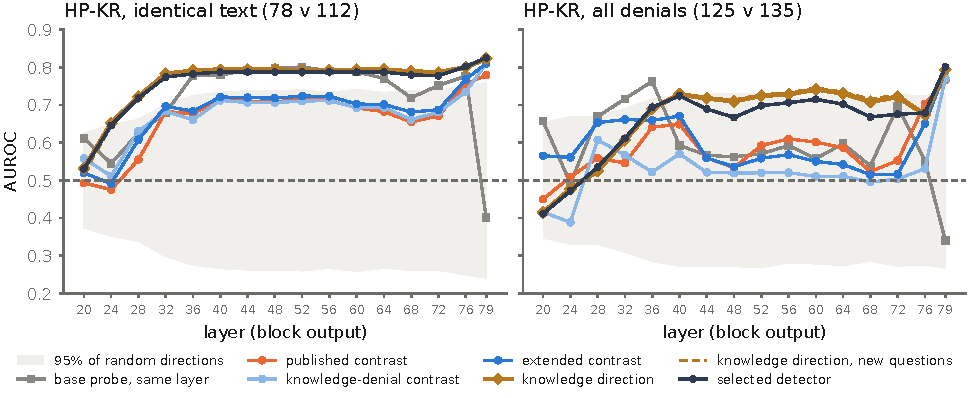
\includegraphics[width=0.78\linewidth]{fig_knowledge_hpkr.pdf}
\caption{\hpkr's wording-controlled slices across the 16 layers; grey marks the central 95\% of random
directions.}
\label{fig:k-hpkr}
\end{figure}

\subsection{The knowledge direction}
\label{sec:knowledge}

On the identical-text slice the knowledge direction reads \V{th-k-k-ident-L40} [\V{th-k-ident-lo-L40},
\V{th-k-ident-hi-L40}], above the band, \V{th-k-ident-nowording-L40} with its wording component removed,
and above the band at \V{th-k-depth-ident-above} of the \V{th-k-depth-n} layers, the replication direction
on the same curve (\cref{fig:k-hpkr}). The slice's lies and honest denials are different questions, so it
cannot separate what the model knows from which questions these are, and the base probe trained at the
same layer is level with the knowledge direction there (\V{th-k-probe-ident-L40}; difference
\V{li-k-vs-probe-ident} [\V{li-k-vs-probe-ident-lo}, \V{li-k-vs-probe-ident-hi}]), though it is trained on
labels and fails on insider trading. On the full \hpkr{} the knowledge direction reads \V{th-k-full-L40},
a number that rests on the words (\V{th-k-full-nowording-L40} without them), so we credit it only with the
slices. Built inside the Gender-Secret fine-tune and read through it, it reads \V{th-k-gs-ft-kft-L40}
[\V{th-k-gs-ft-kft-lo-L40}, \V{th-k-gs-ft-kft-hi-L40}] against a band of \V{th-k-gs-ft-band-L40}, where
the base model's read of the same transcripts gives \V{th-k-gs-base-kft-L40} (\cref{app:organisms}); the
margin is a few hundredths and the classes differ in topic as well as in knowledge. On the five datasets it
averages \V{th-k-k-mean-L40}, below the extended contrast's \V{th-k-dnine-mean-L40}, and it leads the
extended contrast only on \hpc{} (\V{th-k-k-auroc-hpc-L40} against \V{th-k-dnine-auroc-hpc-L40}). These
results rest in part on \hpkr's template: rebuilt without its wording, by a rule chosen on these datasets,
the direction keeps the wording-controlled \hpkr{} results, transfers a little worse here
(\V{xm-llama-rk-off} against \V{th-k-k-off-L40}) and much worse on Mistral (\cref{sec:models}), and on
Gender-Secret falls inside the random band (\V{ru-llama-gs-rule}). Resampling its
questions gives a 95\% interval at most \V{th-k-boot-ident-width} wide on the identical text; none of 1,000
balanced splits of the same questions reaches it, a null adopted after the first-specified random split
proved uninformative; and the replication direction has a cosine of \V{th-k-rep-cos-L40} with the
original, though it was scored on the same test rows.

\subsection{The combined detector and its tail}
\label{sec:combined}

The selected detector transfers at \V{th-k-ninek-off-L40} against \V{off-base-L40} for the raw probe,
level with the extended contrast (\V{xm-llama-ci-off-ninek-dnine} [\V{xm-llama-ci-off-ninek-dnine-lo},
\V{xm-llama-ci-off-ninek-dnine-hi}]), and its five-dataset mean of \V{th-k-ninek-mean-L40} is
\V{th-pair-ninek-dnine-mean-L40} above the contrast with an interval that includes zero
([\V{th-pair-ninek-dnine-mean-lo-L40}, \V{th-pair-ninek-dnine-mean-hi-L40}]). Its case is made where the
words are controlled: it gains \V{th-pair-ninek-dnine-ident-L40} [\V{th-pair-ninek-dnine-ident-lo-L40},
\V{th-pair-ninek-dnine-ident-hi-L40}] on the identical text and \V{th-k-gs-gain-L40} on Gender-Secret,
where with both directions rebuilt in the fine-tune it reads \V{th-k-gs-ft-ninekft-L40}, a few hundredths
above the band (built on the base model it reads \V{th-k-gs-ft-ninek-L40}, inside it), at small costs on
CG, ID and IT. It beats the same-layer base probe on the five-dataset mean by
\V{xm-llama-ci-lb-ninek-probe}, almost all of it on insider trading, where the probe inverts; it is level
with that probe on the identical text and below it on held-out lies (\cref{sec:external}). Across depth it
transfers above the published and unified contrasts and the raw probe at every one of the 16 layers, by at
least \V{th-k-ninek-depth-lead-min} (\cref{app:depth}; point estimates), but averaged over the layers it
transfers below the extended contrast alone (\V{th-k-ninek-depth-off-mean} against \V{th-ext-off-mean};
\V{th-k-ninek-off-L20} against \V{off-ext-L20} at layer~20), and the extended contrast's own transfer peaks at
layer~\V{depth-off-ext-peak-layer} (post hoc). The tail is the weakness: with cutoffs that flag 1\% of a
dataset's own honest answers the extended contrast catches \V{th-k-op-dnine-1-L40} of the lies, the
selected detector \V{th-k-op-ninek-1-L40}, the base probe \V{th-k-op-probe-1-L40} and the knowledge
direction \V{th-k-op-k-1-L40}, and placing the threshold on each dataset instead of on Alpaca changes
balanced accuracy by a few hundredths at most (\cref{tab:oracle}).

\subsection{Steering the persona contrast}
\label{sec:steering}

Adding the extended contrast at $c = +0.3$ cuts disclosure of the hidden fact from \V{th-steer-base} to
\V{th-steer-ext-plus} (\V{th-steer-ext-plus-change} [\V{th-steer-ext-plus-lo}, \V{th-steer-ext-plus-hi}]);
the published contrast does the same (\V{th-steer-dec-plus-change}), two random directions do not, and the
base probe's direction moves it by \V{th-steer-base-plus-change} [\V{th-steer-base-plus-lo},
\V{th-steer-base-plus-hi}] (\cref{app:steering}). The steered answers take on the deceptive personas' manner,
so what the model acts on is plausibly the register of those roles. The result rests on one blinded reader
(an AI assistant), one coefficient and one greedy answer per scenario, and an earlier run with an absolute
shift on benchmark items found nothing beyond random; two small runs that steered the knowledge direction
are suggestive only (\cref{app:steering}).

\section{Across models}
\label{sec:models}

We repeated the studies on Qwen2.5-72B-Instruct, Mistral-Small-3.1-24B-Instruct and Gemma-3-27B-it with
the same code, the blocks and banks fixed before any result was read (\cref{tab:models} in
\cref{app:models}; steering not repeated). Each model has its own bank from the same roles, variants,
questions and judge. In Qwen's strict bank \V{xq-sys-roles-under} roles keep fewer than
\V{xq-strict-min} rollouts scored 3, so Qwen uses the bank that also keeps rollouts scored 2, marked
$\dagger$; the lenient banks of the other three models change the contrasts' means and the extended
contrast's transfer at the middle block by at most \V{xs-bank-gap} (\cref{tab:xm-banks}). \Cref{tab:claims}
checks the claims at each model's middle block; every interval is in \cref{app:models}.

\begin{table}[t]
\centering
\footnotesize
\caption{The claims at each model's middle block: a paired difference, or an AUROC with the value it must
clear (or, for the persona row, stay below) in brackets. \checkmark{} holds, $\times$ does not, $\circ$ no
clear difference (the interval includes zero, or the values are within 0.01). $^\dagger$Qwen's lenient bank.
$^a$Qwen's identical reply, rebuilt from the raw files. $^b$Gemma's opening sentence, rebuilt,
\V{xm-gemma-rb-open-lies} lies. On Gender-Secret the margin is a few hundredths and the classes also differ
in topic.}
\label{tab:claims}
\resizebox{\linewidth}{!}{% Generated by make_xmodel_assets.py from transfer_ci.py, k_robustness.py paired and the slice and organism scores
\begin{tabular}{@{}>{\raggedright\arraybackslash}p{7.2cm} cccc@{}}
\toprule
Claim & Llama & Qwen$^\dagger$ & Mistral & Gemma \\
\midrule
Extended contrast transfers above the probe on raw activations & $+$0.184 \checkmark & $-$0.106 $\times$ & $+$0.094 \checkmark & $+$0.175 \checkmark \\
Extended contrast transfers above the published contrast & $+$0.084 \checkmark & $+$0.002 $\circ$ & $+$0.176 \checkmark & $+$0.221 \checkmark \\
The knowledge-denial roles raise the mean (extended above published) & $+$0.101 \checkmark & $+$0.061 \checkmark & $+$0.043 \checkmark & $+$0.221 \checkmark \\
Extended contrast's mean is above the benchmark's Mean Probe & 0.899 (0.682) \checkmark & 0.441 (0.530) $\times$ & 0.762 (0.570) \checkmark & 0.900 (0.527) \checkmark \\
Selected detector transfers above the probe on raw activations & $+$0.190 \checkmark & $-$0.045 $\times$ & $+$0.125 \checkmark & $+$0.114 \checkmark \\
Selected detector's mean is above the same-block RepE probe & $+$0.128 \checkmark & $+$0.036 \checkmark & $+$0.038 \checkmark & $+$0.064 \checkmark \\
No persona direction clears the band on identical text & 0.721 (0.733) \checkmark & 0.550 (0.584)$^a$ \checkmark & 0.784 (0.755) $\times$ & 0.624 (0.622)$^b$ $\circ$ \\
Knowledge direction clears the band on identical text & 0.793 (0.733) \checkmark & 0.602 (0.584)$^a$ \checkmark & 0.840 (0.755) \checkmark & 0.585 (0.622)$^b$ $\times$ \\
Knowledge direction clears the band on Gender-Secret, read through the fine-tune & 0.861 (0.824) \checkmark & n/a & 0.440 (0.765) $\times$ & n/a \\
\bottomrule
\end{tabular}
}
\end{table}

\paragraph{What carries over.} On Mistral and Gemma the extended contrast transfers above the raw probe
(by \V{xm-mistral-ci-off-dnine-raw} and \V{xm-gemma-ci-off-dnine-raw}, intervals above zero) and above
the published contrast. Zero-shot, its mean over the model's datasets is well above the benchmark's
layer-20 Mean Probe on both (\V{xm-mistral-lb-dnine} against \V{xm-mistral-lb-meanprobe};
\V{xm-gemma-lb-dnine} against \V{xm-gemma-lb-meanprobe}); against the base probe trained at the same block
it is above on Gemma (\V{xs-gemma-dnine-probe} [\V{xs-gemma-dnine-probe-lo}, \V{xs-gemma-dnine-probe-hi}])
and level on Mistral (\V{xs-mistral-dnine-probe} [\V{xs-mistral-dnine-probe-lo},
\V{xs-mistral-dnine-probe-hi}]). Adding our ten roles raises the contrast's mean over the published
contrast on all four models (by \V{xm-llama-ci-lb-dnine-dfive}, \V{xm-qwen-ci-lb-dnine-dfive},
\V{xm-mistral-ci-lb-dnine-dfive} and \V{xm-gemma-ci-lb-dnine-dfive}), though on Llama about one random
widening in six of a random bank gains as much (\cref{sec:external}), so the gain is not shown to be
specific to these roles. The selected detector's mean over the benchmark's datasets is above the same-block
probe's on all four (by \V{xm-llama-ci-lb-ninek-probe}, \V{xm-qwen-ci-lb-ninek-probe},
\V{xm-mistral-ci-lb-ninek-probe} and \V{xm-gemma-ci-lb-ninek-probe}; on Qwen both are near chance), while
on the held-out lies of Llama and Gemma the probe is ahead (\V{ai-probe} against \V{ai-ninek};
\V{xm-gemma-aisi-probe} against \V{xm-gemma-aisi-ninek}). Adding the knowledge direction leaves transfer
level on Llama, raises it on Mistral (\V{xm-mistral-ci-off-ninek-dnine}) and Qwen (to \V{xm-qwen-off-ninek},
still below the raw probe) and lowers it on Gemma (\V{xm-gemma-ci-off-ninek-dnine}), where the knowledge
direction alone is weak.

\paragraph{Qwen: the persona contrast fails.} On Qwen the extended contrast transfers below the raw probe
(\V{xm-qwen-off-dnine} against \V{xm-qwen-off-raw}), is level with the published contrast, averages
\V{xm-qwen-lb-dnine} zero-shot against the Mean Probe's \V{xm-qwen-lb-meanprobe}, and inverts on \hpkr{}
(\V{xm-qwen-hpkr-dnine}); the failure is \hpkr's, since with \hpkr{} left out it transfers above the raw
probe (\V{xq-s23-offx-dnine} against \V{xq-s23-offx-raw}), and the knowledge-denial contrast is the
exception (transfer \V{xm-qwen-off-deight}, \hpkr{} \V{xm-qwen-hpkr-deight}). The judge scored
\V{xm-qwen-roleplay}\% of Qwen's rollouts fully in role, against \V{xm-llama-roleplay}\%,
\V{xm-mistral-roleplay}\% and \V{xm-gemma-roleplay}\% for Llama, Mistral and Gemma (by group in
\cref{tab:xm-roleplay}), which suggested that the contrast fails because Qwen does not play the roles. A second Qwen bank, built after these results with
the role line and a stay-in-character sentence in the user turn, rules that out as the whole story: Qwen
plays \V{xq-s3u-roleplay}\% of its rollouts fully in role, every role keeps enough to enter the strict bank,
and the extended contrast still transfers below the raw probe (\V{xq-s3u-off-dnine} against
\V{xq-s3u-off-raw}; \V{xq-s3u-ci-dnine-raw} [\V{xq-s3u-ci-dnine-raw-lo}, \V{xq-s3u-ci-dnine-raw-hi}]),
again because of \hpkr{} (\V{xq-s3u-offx-dnine} against \V{xq-s3u-offx-raw} without it), while the
knowledge-denial contrast transfers (\V{xq-s3u-off-deight}). Why the published roles invert on Qwen's \hpkr{}
is open; that a model plays the roles is not enough for a persona contrast to transfer.

\paragraph{The knowledge direction across models.} On Mistral, the one other model with a released
identical-text slice (\V{xm-mistral-ident-lies} lies v \V{xm-mistral-ident-honest} honest), the knowledge
direction reads \V{xm-mistral-ident-k} against a band of \V{xm-mistral-ident-band}, above the same-block
probe by \V{xm-mistral-ci-ident-k-probe} [\V{xm-mistral-ci-ident-k-probe-lo},
\V{xm-mistral-ci-ident-k-probe-hi}] and above its band at all \V{xm-mistral-depth-ident-above} depths; on
Qwen's rebuilt identical reply it reads \V{xm-qwen-rb-ident-k} [\V{xm-qwen-rb-ident-k-lo},
\V{xm-qwen-rb-ident-k-hi}] against \V{xm-qwen-rb-ident-band}, narrowly; on Gemma's \V{xm-gemma-rb-open-lies}
rebuilt lies it is inside the band (\V{xm-gemma-rb-open-k} against \V{xm-gemma-rb-open-band}), too few to
decide. The register diagnosis holds on Qwen's rebuilt reply, where every persona direction is inside the
band, but only in part on Mistral: the knowledge-denial contrast flags \V{xm-mistral-flag-hden-deight}\% of
the honest denials and sits inside the band on the identical text, the extended contrast is at its edge
(\V{xm-mistral-ident-dnine}), and the published contrast is above it (\V{xm-mistral-ident-dfive}), so the
check fails there. Alone on the datasets the knowledge direction averages \V{xm-mistral-lb-k} on Mistral but
\V{xm-qwen-lb-k} on Qwen and \V{xm-gemma-lb-k} on Gemma, where it inverts on instructed deception
(\V{xm-gemma-k-id}) and on Gemma's own held-out lies (\V{xm-gemma-aisi-k}). The fine-tunes add no evidence
for it, and Mistral's Gender-Secret, the one replication of Llama's test, counts against it
(\V{xm-mistral-gs-k} against a band of \V{xm-mistral-gs-band}); on the Soft-Trigger fine-tunes the base
model's read already separates the classes or the direction stays inside the band (\cref{app:organisms}).
A \emph{template-free} knowledge direction, built with none of \hpkr's wording, keeps the wording-controlled
\hpkr{} results on Mistral (identical text \V{xm-mistral-rk-ident}, by a rule fixed before Mistral was read)
and on Llama (\V{xm-llama-rk-ident}, though there the rule's wording was chosen with Llama's own datasets in
view), but transfers worse (\V{xm-mistral-rk-off} against \V{xm-mistral-off-k} on Mistral), so only those
slices are free of the template.

\paragraph{Across depth and what generalises.} The middle block was fixed in advance but need not be
where a model's signal is (\cref{app:models}): the extended contrast transfers above the raw probe, by any
margin, at all \V{xm-llama-depth-n} depths on Llama but at \V{xm-mistral-depth-above} of 16 on Mistral,
\V{xm-gemma-depth-above} on Gemma and \V{xm-qwen-depth-above} on Qwen, where it stays near chance until
\V{xm-qwen-depth-rise-rel} of the depth and then reaches \V{xm-qwen-depth-peak}, level with the raw probe
there, at a block found only by looking. Three results hold on every model where they could be tested:
adding the knowledge-denial roles raises the contrast's mean; the selected detector's mean over the
benchmark's datasets is above the same-block probe's; and, where the words are fixed and there are enough
lies, the knowledge direction separates lies from identical honest denials (Llama, Mistral and narrowly
Qwen). The persona contrast's lead in transfer replicates on Mistral and Gemma, not on Qwen; the lead at
every layer, the detection of Gender-Secret through the fine-tune, and the value of adding the knowledge
direction do not generalise.

\section{External and pre-registered tests}
\label{sec:external}

\paragraph{Held-out lies.} On the AISI rollouts' validation split of Llama's own belief-labelled lies
(\V{th-aisi-val-lies} lies, \V{th-aisi-val-honest} honest answers, under system prompts no part of this
work used), the extended contrast reads \V{ai-d9}, the selected detector \V{ai-ninek} and the knowledge
direction \V{ai-k} at layer~40, while the base probe trained on RepE at the same layer reads \V{ai-probe}:
level with the extended contrast, which leads it by \V{ai-d9-delta} [\V{ai-d9-lo}, \V{ai-d9-hi}], and above
the selected detector, which trails it by \V{ai-ninek-gap} [\V{ai-ninek-gap-lo}, \V{ai-ninek-gap-hi}]. A
base probe trained on a split of \V{th-aisi-train-rows} of Llama's own rollouts (\V{th-aisi-train-lies}
lies, disjoint from the validation split) raises the five-dataset mean by \V{th-aisi-gain-L40}
[\V{th-aisi-gain-lo-L40}, \V{th-aisi-gain-hi-L40}] over the RepE probe; the extended contrast is narrowly
ahead of it at layer~40 (\V{th-aisi-ext-L40} [\V{th-aisi-ext-lo-L40}, \V{th-aisi-ext-hi-L40}]), level at
layer~44, and clearly ahead only at layer~20 (\V{th-aisi-ext-L20}). The template-free knowledge direction
loses here (\V{ai-rulek} against \V{ai-k}).

\paragraph{The random persona bank.} Six tests were fixed before scoring (\cref{app:random}). The extended
contrast beats the random 12 v 13 contrasts on transfer (\V{rb-t1-d} against a null 97.5th percentile of
\V{rb-t1-null}), on the zero-shot five-dataset mean (\V{rb-t2-d} against \V{rb-t2-null}), with the
knowledge direction added (\V{rb-t3-d} against \V{rb-t3-null}) and on the held-out lies (\V{rb-t6-d}
against \V{rb-t6-null}), each at a Holm-corrected $p$ of \V{rb-t1-p}. Two tests fail: its AUROC on all of
\hpkr{} (\V{rb-t4-d}) is inside the null (97.5th percentile \V{rb-t4-null}, $p$ = \V{rb-t4-p}), and the
gain of the extended over the published contrast on the five-dataset mean (\V{rb-t5-d}) is within what
widening a random 8 v 7 contrast by four and six random roles, our groups' sizes, produces (null median
\V{rb-t5-null-median}, 97.5th percentile \V{rb-t5-null}, $p$ = \V{rb-t5-p}), so the size of our roles' gain
cannot be told apart from the spread of random widenings.

\paragraph{Aletheia's Quest.} The competition \citep{aletheia2026quest} scored lie detectors on ten
held-out datasets of fine-tuned organisms and prompted liars built on Qwen3.5-27B, Gemma-3-27B and a
Nemotron model, ranked by mean AUROC. We built a persona bank on Qwen3.5-27B and on Gemma-3-27B by the
pipeline above and a knowledge direction inside each organism, froze a protocol before any test row was
read, and scored the selected detector zero-shot as read by each organism (adapter, merged copy or, for the one
dataset plain Gemma wrote, base Gemma) at the middle block, reasoning dropped as in the starter kit. Two Hidden-Goal datasets could not be read
(gated adapters; the Nemotron one would also have needed a persona bank, which we did not build). Over the
\V{ax-n-read} readable datasets (\cref{tab:aletheia} in \cref{app:aletheia}) the selected detector averages
\V{ax-headline-mean} [\V{ax-headline-lo}, \V{ax-headline-hi}], which would place it \V{ax-headline-rank}th
among the \V{ax-n-entries} published entries with their means recomputed over the same eight datasets
(rank interval \V{ax-rank-lo} to \V{ax-rank-hi}); the extended contrast alone averages \V{ax-d9-mean}
(\V{ax-d9-rank}th) and the RepE probe trained at the same block \V{ax-repe-mean} (\V{ax-repe-rank}th). With
the reasoning tokens kept, a secondary cell, the selected detector reaches \V{ax-reasoning-mean}
(\V{ax-reasoning-rank}th) and the extended contrast \V{ax-reasoning-d9-mean} (\V{ax-reasoning-d9-rank}rd).
The selected detector is below chance on two organisms, Echoblast (\V{ax-echo-headline}; knowledge direction
alone \V{ax-echo-k}) and AuditBench's hallucinated citations (\V{ax-abhc-headline}; \V{ax-abhc-k}). The top
entries are active methods, such as the suspect model judging its own transcript, where this detector is
one passive inner product; two deviations from the frozen protocol are recorded in \cref{app:aletheia}.

\paragraph{The 150-question extension.} The bank's 30 shared questions are all first-person workplace
advice. We pre-registered an extension to 150: 30 monotone questions in the originals' form, a control for
count, and 90 diverse questions over a grid of manipulation type, deceiver, topic and format, frozen before
generation (\V{qb-rollouts} rollouts; development on the five benchmark datasets at layer~40, then one
confirmation read; \cref{app:qbank}). Variety did not beat count: the originals plus the 30 monotone
questions give a five-dataset mean of \V{qb-t1-mono} against a median of \V{qb-t1-median} over 200 draws of
the originals plus 30 random diverse questions (Holm-corrected $p$ = \V{qb-t1-holm}). Pooling all 150 gives a
worse contrast (\V{qb-pooled-lb}) than the best single family (\V{qb-best-family-lb}; \V{qb-t3-delta}
[\V{qb-t3-lo}, \V{qb-t3-hi}]): against the 30 originals the full 150 raise CG (\V{qb-b150-b30-d9-cg}) and cut
\hpkr{} (\V{qb-b150-b30-d9-hpkr}), the diverse questions driving most of the first and all of the second,
the loss most of all from questions on which an honest role truthfully says ``I don't know''. A
covariance-weighted cosine predicts which family transfers where better than the plain cosine ($R^2$
\V{qb-t4-r2-sigma} against \V{qb-t4-r2-plain}), though with a near-perfect target probe it is close to the
detector's own effect size (\cref{app:side}). With the knowledge direction the four candidate banks lie within
\V{qb-decision-spread}, so the 150-question bank was chosen by the pre-registered tie rule; its one
confirmation read at layer~40 is better on the held-out lies by \V{qb-confirm-aisi-ninek-delta}
[\V{qb-confirm-aisi-ninek-lo}, \V{qb-confirm-aisi-ninek-hi}] and worse on Gender-Secret by
\V{qb-confirm-gs-ninek-gap} [\V{qb-confirm-gs-ninek-gap-lo}, \V{qb-confirm-gs-ninek-gap-hi}]. A Qwen3.5-27B
leg is still running.

\section{Discussion and conclusion}
\label{sec:discussion}

A persona direction responds to how a reply is worded more than to whether it is a lie: where the words
are fixed the persona directions are inside the random band on Llama and Qwen and at or above its edge on
Mistral. And what makes a lie a lie, that the speaker knows otherwise, can be read directly where
the words are held fixed: the knowledge direction separates identical denials on Llama, Mistral and
narrowly Qwen. Neither is a mechanism. Beyond those slices the knowledge direction is narrower than we
first thought: its transfer rests on the benchmark's request line, its fine-tune result on one model, and
on Gemma and on two competition organisms it points the wrong way. Three checks follow: test a persona
direction where lies and honest answers share their words, against the random band and a random bank
built by the same pipeline, and on every new model; accept a model organism as a test only if the base model's read of its transcripts cannot already separate the
classes; and keep ranking apart from detecting.

\paragraph{Limitations.} The knowledge-denial roles and the knowledge direction were designed after
\hpkr{} was seen to fail, so \hpkr{} is a repair, not a blind test; the held-out lies, Gender-Secret, the
random bank and the pre-registered tests carry the untargeted evidence. The base probe trained at the same
layer is level with the knowledge direction on Llama's identical text and with the extended contrast on
the held-out lies, and ahead of the selected detector there and on the competition: the label-free
directions' advantage is transfer across kinds of lie, not a general lead over supervision. On Llama,
Gender-Secret is the one organism that credits the knowledge direction, by a few hundredths, its classes
also differing in topic, and on Mistral the same organism counts against it; on the identical-text slices
lies and honest denials are different questions; intervals resample rows, not datasets; the
steering labels come from single readers (in the main run an AI assistant reading blind); and everything is
in English. Open are Qwen's failure, a
knowledge direction whose transfer survives a change of wording, and combining these passive reads with the
active, self-evaluating monitors that led the competition.


\subsubsection*{Reproducibility statement}

Every \verb|\V| number in this paper, and every table and figure, is written by the generators named in
\cref{app:repro}, from result files or, for a few run counts, from the studies' reports; the build stops if
a key is missing or a claim the generator asserts no longer holds. The side studies summarised in \cref{app:side} and the knowledge-direction steering runs in
\cref{app:steering} are quoted from their report files. The persona bank's roles and prompts, the knowledge
direction's questions and templates, the pre-registration documents of the competition protocol and of the
question extension, and the code for every experiment are at \repourl. All forward passes ran on the
National Deep Inference Fabric through nnsight; the analysis runs on pooled activations on a CPU.
\Cref{app:repro} lists the bootstrap scheme, the random-direction construction, the block mapping for each
model and the data revisions.

\subsubsection*{Ethics statement}

The harm-pressure datasets contain hazardous questions from WMDP; we quote none of them and withhold the
hazardous content from every example. Lie detectors are dual-use: a monitor that reads whether a model
conceals knowledge could also be turned on honest refusals. We report where the detectors fail as
prominently as where they succeed, so that no reader takes a single label-free direction for a reliable
monitor. No human subjects were involved.

\subsubsection*{AI use statement}

% Authors: confirm and edit this statement before submission. Items still to confirm: who wrote the
% knowledge direction's 120 questions (recall_items.py and recall_items_matched.py); who read the two
% knowledge-direction steering runs by hand (results/steering_L40_knowledge, steering_L40_gender_secret);
% and whether a human should re-label the steering answers (steering_L40_notebook/blind_reading_sheet.md).
We used an AI coding assistant (Claude, Anthropic) for much of the implementation and analysis code, for
drafting and editing the text, and for literature search. Every analysis script was run by us on the stated
data, and every number in the paper is read from the resulting files by the generators described above. The
AI assistant also produced evaluation data in two places, both disclosed where they are used: the 120 new
questions of the question extension were written by it under a fixed prompt archived with the
pre-registration (\cref{app:qbank}), and the disclosure labels of the steering experiment are one blinded
reading by it against a hidden key (\cref{sec:method}). The
persona rollouts are generated and judged by the open models named in \cref{sec:method}, as part of the
method. We checked the AI-assisted code, data and text and take responsibility for the final content.

\ifanonymous\else
\subsubsection*{Acknowledgements}

The large-model experiments ran on the National Deep Inference Fabric (NDIF), which gave remote access to
the internals of models that would otherwise have been out of reach on the hardware available to us.
\fi


\bibliography{refs}
\bibliographystyle{iclr2027_conference}

\appendix
% Appendices. Each table is a generated file; the text around it says what it adds to the main text.

\FloatBarrier
\section{The persona bank}
\label{app:bank}

\Cref{tab:roster} lists the 36 roles by group. The 26 published roles follow the descriptions of
\citet{mahadik2026persona}; the ten knowledge-denial, sincere-ignorance and plain-assertion roles are ours.
Each role has five system-prompt variants and answers the same 30 questions; a Llama-3.1-70B-Instruct
judge scores each rollout from 0 to 3, and only rollouts scored 3 enter a persona vector.
\Cref{tab:xm-roleplay} gives the share of rollouts each model plays fully in role by persona group, and
\cref{tab:xm-banks} the lenient (score 2 to 3) banks beside the strict ones.

\begin{table}[h]
\centering
\scriptsize
\caption{The roles of the bank by group.}
\label{tab:roster}
\resizebox{\linewidth}{!}{% Generated by make_numbers.py
\begin{tabularx}{\linewidth}{@{}lc>{\raggedright\arraybackslash}X@{}}
\toprule
Group & $n$ & Personas (kept rollouts) \\
\midrule
Deceptive (published) & 8 & handler (106), broker (113), impression manager (82), coverup operator (47), gatekeeper (126), spin doctor (85), plausible denier (64), narrative manager (70) \\
Honest (published) & 7 & archivist (103), disclosure counsel (118), documentarian (107), fact checker (48), ombudsman (148), transparency officer (142), whistleblower (108) \\
Knowledge denial (new) & 4 & amnesiac witness (129), deniable expert (72), feigned novice (137), stonewaller (129) \\
Sincere ignorance (new) & 3 & honest novice (110), calibrated reporter (83), scrupulous witness (74) \\
Plain assertion (new) & 3 & forthright expert (80), candid witness (64), plain dealer (76) \\
Sycophantic (published) & 5 & cheerleader (142), enabler (51), flatterer (148), people pleaser (113), yes man (109) \\
Anti-sycophantic (published) & 5 & blunt advisor (135), contrarian (130), critic (68), skeptic (133), tough love mentor (149) \\
Anchor & 1 & default (150) \\
\bottomrule
\end{tabularx}}
\end{table}

\begin{table}[h]
\centering
\footnotesize
\caption{The share of rollouts the judge scored fully in role, by persona group and model.}
\label{tab:xm-roleplay}
% Generated by make_xmodel_assets.py from the judge's scores
\begin{tabular}{@{}l cccc@{}}
\toprule
Persona group & Llama & Qwen$^\dagger$ & Mistral & Gemma \\
\midrule
Deceptive (published contrast) & 58\% & 15\% & 73\% & 97\% \\
Honest (published contrast) & 74\% & 52\% & 85\% & 99\% \\
Knowledge-denial (knowledge-denial contrast) & 78\% & 10\% & 54\% & 96\% \\
Knowledge-candour (knowledge-denial contrast) & 54\% & 22\% & 53\% & 89\% \\
Sycophantic & 75\% & 37\% & 60\% & 97\% \\
Anti-sycophantic & 82\% & 28\% & 75\% & 100\% \\
\midrule All 35 roles & 69\% & 28\% & 68\% & 96\% \\
\bottomrule
\end{tabular}

\end{table}

\begin{table}[h]
\centering
\footnotesize
\caption{Each model's persona banks at its middle block: the strict bank and the lenient one.}
\label{tab:xm-banks}
\resizebox{\linewidth}{!}{% Generated by make_xmodel_assets.py from bank_comparison
\begin{tabular}{@{}ll cccc@{}}
\toprule
 & & \multicolumn{3}{c}{Mean over the model's datasets} & \\
\cmidrule(lr){3-5}
Model & Bank & Published contrast & Knowledge-denial contrast & Extended contrast & Extended contrast transfer \\
\midrule
Llama & score 3 & 0.798 & 0.894 & 0.899 & 0.916 \\
 & scores 2--3 & 0.786 & 0.880 & 0.888 & 0.907 \\
Qwen$^\dagger$ & score 3 & n/a & n/a & n/a & n/a \\
 & scores 2--3 & 0.380 & 0.668 & 0.441 & 0.453 \\
Mistral & score 3 & 0.719 & 0.727 & 0.762 & 0.810 \\
 & scores 2--3 & 0.712 & 0.747 & 0.770 & 0.816 \\
Gemma & score 3 & 0.679 & 0.484 & 0.900 & 0.921 \\
 & scores 2--3 & 0.684 & 0.487 & 0.895 & 0.912 \\
\bottomrule
\end{tabular}
}
\end{table}

\FloatBarrier
\section{Llama: supplementary results}
\label{app:llama}

\Cref{tab:designs} places the designs side by side at layer~40, \cref{fig:transfer} shows the transfer
matrices of the raw probe and the selected detector, \cref{tab:evalsets} lists the evaluation sets,
\cref{tab:knowledge} every detector on every set at layer~40, \cref{tab:zeroshot} the three persona contrasts at layers 20, 40 and 44, \cref{tab:transfer}
transfer for every feature set, and \cref{tab:hpkr} \hpkr{} ranking against detection beside the
benchmark's published probes. \Cref{tab:pertest} gives every detector's AUROC on every dataset at the
three layers, \cref{tab:syc} the sycophancy and unified contrasts, \cref{tab:reads} the token reads,
\cref{tab:followup} the read at the Follow-Up turn's ``No'', and \cref{tab:kthree} probes in three persona
components.

\begin{table}[h]
\centering
\footnotesize
\caption{The designs at layer 40: transfer (train one, test all, over the six sets), the zero-shot
five-dataset mean with balanced accuracy (BA) at the benchmark's threshold, and \hpkr{} on all rows and on
its identical-text slice.}
\label{tab:designs}
\resizebox{\linewidth}{!}{% Generated by make_thesis_assets.py
\begin{tabular}{@{}l l cc cc cc@{}}
\toprule
& & \multicolumn{2}{c}{Transfer AUROC} & \multicolumn{2}{c}{Five-dataset mean} & \multicolumn{2}{c}{\hpkr{} AUROC} \\
\cmidrule(lr){3-4}\cmidrule(lr){5-6}\cmidrule(lr){7-8}
Design & Labels & all six & excl.\ \hpkr{} & AUROC & BA & all & identical \\
\midrule
Probe on raw activations & one dataset & 0.732 & 0.758 & n/a & n/a & n/a & n/a \\
Base probe (RepE) & RepE & n/a & n/a & 0.778 & 0.626 & 0.936 & 0.779 \\
Base probe, own lies (AISI) & AISI & n/a & n/a & 0.878 & 0.630 & 0.935 & 0.686 \\
Persona method, extended PCs ($k=3$) & one dataset & 0.866 & 0.867 & n/a & n/a & n/a & n/a \\
Published contrast & none & 0.832 & 0.880 & 0.798 & 0.675 & 0.593 & 0.715 \\
Sycophancy contrast & none & 0.663 & 0.936 & 0.770 & 0.601 & 0.167 & 0.686 \\
Unified contrast & none & 0.690 & 0.919 & 0.795 & 0.655 & 0.381 & 0.707 \\
Knowledge-denial contrast & none & 0.912 & 0.910 & 0.894 & 0.725 & 0.919 & 0.712 \\
Extended contrast & none & 0.916 & 0.917 & 0.899 & 0.694 & 0.912 & 0.721 \\
\midrule
Knowledge direction & none & 0.823 & 0.815 & 0.825 & 0.553 & 0.865 & 0.793 \\
Published contrast + knowledge direction & none & n/a & n/a & 0.879 & 0.646 & 0.854 & 0.789 \\
Selected detector (extended + knowledge) & none & 0.922 & 0.924 & 0.906 & 0.701 & 0.909 & 0.787 \\
\bottomrule
\end{tabular}
}
\end{table}

\begin{figure}[h]
\centering
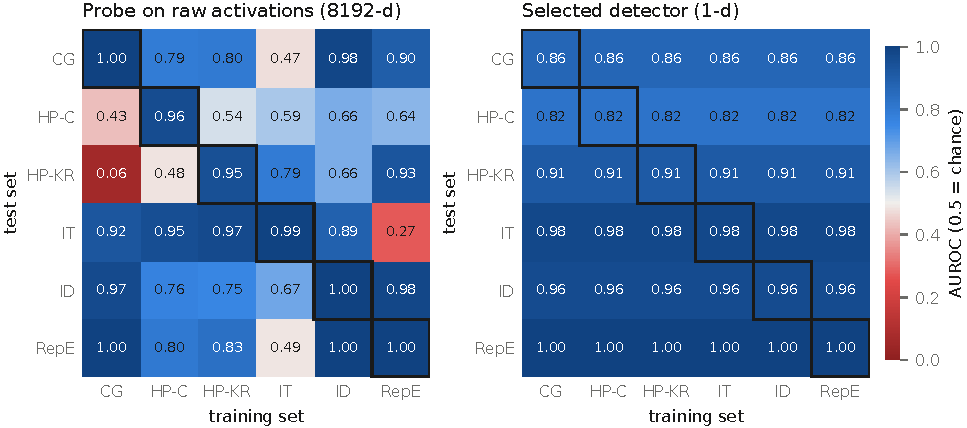
\includegraphics[width=\linewidth]{fig_transfer_selected.pdf}
\caption{Train-one-test-all AUROC at layer 40 for the probe on raw activations (left) and the selected
detector (right), whose rows are constant off the diagonal because every training set agrees on its sign.}
\label{fig:transfer}
\end{figure}

\begin{table}[h]
\centering
\footnotesize
\caption{The evaluation sets for Llama-3.3-70B-Instruct.}
\label{tab:evalsets}
% Generated by make_numbers.py
\begin{tabular}{llllrr}
\toprule
Dataset & Short & Object of belief & Reason for lying & Examples & Lies \\
\midrule
Convincing-Game & CG & self-knowledge & encouraged & 267 & 167 \\
Harm-Pressure Choice & HP-C & world-knowledge & inherent & 2,134 & 134 \\
Harm-Pressure Knowledge Report & HP-KR & self-knowledge & inherent & 2,139 & 139 \\
Insider-Trading & IT & self-knowledge & encouraged & 1,080 & 423 \\
Instructed-Deception & ID & world-knowledge & encouraged & 5,432 & 3,045 \\
\midrule
RepE instruction pairs & RepE & world-knowledge & instructed & 550 & 275 \\
Alpaca (control) & n/a & n/a & none & 2,000 & 0 \\
\bottomrule
\end{tabular}
\end{table}

\begin{table}[h]
\centering
\footnotesize
\caption{AUROC at layer 40; the Mean Probe is Liars' Bench's layer-20 probe. On Gender-Secret the
directions are built inside the fine-tune.}
\label{tab:knowledge}
% Generated by make_thesis_assets.py
\begin{tabular}{@{}l ccc ccc@{}}
\toprule
 & \multicolumn{2}{c}{Trained on RepE} & \multicolumn{3}{c}{Zero-shot, layer 40} \\
\cmidrule(lr){2-3}\cmidrule(lr){4-6}
Evaluation set & Mean Probe & \shortstack{base probe,\\layer 40} & \shortstack{extended\\contrast} & \shortstack{knowledge\\direction} & \shortstack{selected\\detector} \\
\midrule
CG & 1.00 & 0.972 & 0.912 & 0.641 & 0.865 \\
HP-C & 0.41 & 0.675 & 0.712 & 0.830 & 0.820 \\
HP-KR & 0.12 & 0.936 & 0.912 & 0.865 & 0.909 \\
IT & 0.93 & 0.338 & 0.980 & 0.881 & 0.975 \\
ID & 0.95 & 0.971 & 0.978 & 0.906 & 0.962 \\
Mean of the five & 0.682 & 0.778 & 0.899 & 0.825 & 0.906 \\
\midrule
\hpkr, identical text & n/a & 0.779 & 0.721 & 0.793 & 0.787 \\
\hpkr, denials & n/a & 0.593 & 0.670 & 0.728 & 0.724 \\
Gender-Secret & 0.45 & 0.524 & 0.547 & 0.861 & 0.841 \\
\bottomrule
\end{tabular}

\end{table}

\begin{table}[h]
\centering
\footnotesize
\caption{The published (8 v 7), knowledge-denial (4 v 6) and extended (12 v 13) contrasts, zero-shot.}
\label{tab:zeroshot}
% Generated by make_numbers.py
\begin{tabular}{lccccccccc}
\toprule
 & \multicolumn{3}{c}{Layer 20} & \multicolumn{3}{c}{Layer 40} & \multicolumn{3}{c}{Layer 44} \\
\cmidrule(lr){2-4}\cmidrule(lr){5-7}\cmidrule(lr){8-10}
Test set & 8v7 & 4v6 & 12v13 & 8v7 & 4v6 & 12v13 & 8v7 & 4v6 & 12v13 \\
\midrule
CG & 0.940 & 0.931 & 0.969 & 0.865 & 0.902 & 0.912 & 0.819 & 0.858 & 0.859 \\
HP-C & 0.717 & 0.585 & 0.639 & 0.581 & 0.755 & 0.712 & 0.607 & 0.725 & 0.712 \\
HP-KR & 0.148 & 0.890 & 0.882 & 0.593 & 0.919 & 0.912 & 0.589 & 0.908 & 0.894 \\
IT & 0.988 & 0.976 & 0.990 & 0.979 & 0.913 & 0.980 & 0.979 & 0.933 & 0.982 \\
ID & 0.959 & 0.932 & 0.954 & 0.974 & 0.980 & 0.978 & 0.962 & 0.978 & 0.974 \\
RepE & 0.994 & 0.882 & 0.991 & 1.000 & 1.000 & 1.000 & 1.000 & 1.000 & 1.000 \\
\midrule
Mean & 0.791 & 0.866 & 0.904 & 0.832 & 0.912 & 0.916 & 0.826 & 0.900 & 0.903 \\
\bottomrule
\end{tabular}
\end{table}

\begin{table}[h]
\centering
\footnotesize
\caption{Transfer (mean off-diagonal AUROC) for every feature set, with and without \hpkr.}
\label{tab:transfer}
% Generated by make_numbers.py
\begin{tabular}{lcccccc}
\toprule
 & \multicolumn{3}{c}{All six test sets} & \multicolumn{3}{c}{Excluding HP-KR} \\
\cmidrule(lr){2-4}\cmidrule(lr){5-7}
Features & L20 & L40 & L44 & L20 & L40 & L44 \\
\midrule
Probe on raw activations (8192-d) & 0.648 & 0.732 & 0.716 & 0.728 & 0.758 & 0.730 \\
\midrule
Published contrast, 8 v 7 (1-d) & 0.651 & 0.832 & 0.826 & 0.919 & 0.880 & 0.873 \\
Knowledge-denial contrast, 4 v 6 (1-d) & 0.866 & 0.912 & 0.900 & 0.861 & 0.910 & 0.899 \\
Extended contrast, 12 v 13 (1-d) & 0.904 & 0.916 & 0.903 & 0.909 & 0.917 & 0.905 \\
Selected detector (1-d) & 0.811 & 0.922 & 0.915 & 0.876 & 0.924 & 0.918 \\
\midrule
Extended PCs ($k=3$) & 0.684 & 0.866 & 0.880 & 0.900 & 0.867 & 0.870 \\
Extended PC1 & 0.661 & 0.768 & 0.780 & 0.682 & 0.774 & 0.793 \\
Published PCs ($k=3$) & 0.679 & 0.639 & 0.617 & 0.888 & 0.751 & 0.728 \\
Random directions ($k=3$) & 0.527 & 0.504 & 0.493 & 0.560 & 0.544 & 0.547 \\
\bottomrule
\end{tabular}

\end{table}

\begin{table}[h]
\centering
\footnotesize
\caption{\hpkr: ranking and detection at the benchmark's threshold, beside its published probes.
$^\dagger$Trained with privileged \hpkr{} examples, a ceiling rather than a rival.}
\label{tab:hpkr}
% Generated by make_numbers.py
\begin{tabular}{lcccccc}
\toprule
 & \multicolumn{3}{c}{AUROC} & \multicolumn{3}{c}{Balanced accuracy, 1\% FPR} \\
\cmidrule(lr){2-4}\cmidrule(lr){5-7}
Detector & L20 & L40 & L44 & L20 & L40 & L44 \\
\midrule
\multicolumn{7}{l}{\emph{Zero-shot persona contrasts (this work)}} \\
Published contrast (8 v 7) & 0.148 & 0.593 & 0.589 & 0.500 & 0.500 & 0.500 \\
Knowledge-denial contrast (4 v 6) & 0.890 & 0.919 & 0.908 & 0.533 & 0.910 & 0.757 \\
Extended contrast (12 v 13) & 0.882 & 0.912 & 0.894 & 0.500 & 0.500 & 0.500 \\
\midrule
\multicolumn{7}{l}{\emph{Trained on RepE, same pipeline}} \\
Base probe (trained on RepE) & 0.109 & 0.936 & 0.828 & 0.500 & 0.500 & 0.500 \\
\midrule
\multicolumn{7}{l}{\emph{Reported by Liars' Bench for Llama-3.3-70B (its Tables 6--8)}} \\
Mean Probe & \multicolumn{3}{c}{0.12} & \multicolumn{3}{c}{0.50} \\
Follow-Up Probe & \multicolumn{3}{c}{0.14} & \multicolumn{3}{c}{0.26} \\
Upper-Bound Probe$^\dagger$ & \multicolumn{3}{c}{0.97} & \multicolumn{3}{c}{0.95} \\
\bottomrule
\end{tabular}
\end{table}

\begin{table}[h]
\centering
\scriptsize
\caption{Every detector on every dataset at layers 20, 40 and 44.}
\label{tab:pertest}
\resizebox{\linewidth}{!}{% Generated by make_numbers.py
\begin{tabular}{lcccccc}
\toprule
 & \multicolumn{2}{c}{Layer 20} & \multicolumn{2}{c}{Layer 40} & \multicolumn{2}{c}{Layer 44} \\
\cmidrule(lr){2-3}\cmidrule(lr){4-5}\cmidrule(lr){6-7}
Test set & raw & 12v13 & raw & 12v13 & raw & 12v13 \\
\midrule
CG & 0.663 & 0.969 & 0.787 & 0.912 & 0.757 & 0.859 \\
HP-C & 0.535 & 0.639 & 0.571 & 0.712 & 0.570 & 0.712 \\
HP-KR & 0.394 & 0.882 & 0.584 & 0.912 & 0.637 & 0.894 \\
IT & 0.799 & 0.990 & 0.800 & 0.980 & 0.736 & 0.982 \\
ID & 0.778 & 0.954 & 0.827 & 0.978 & 0.808 & 0.974 \\
RepE & 0.718 & 0.991 & 0.824 & 1.000 & 0.785 & 1.000 \\
\bottomrule
\end{tabular}}
\end{table}

\begin{table}[h]
\centering
\footnotesize
\caption{The sycophancy and unified contrasts.}
\label{tab:syc}
\resizebox{\linewidth}{!}{% Generated by make_numbers.py
\begin{tabular}{lccc}
\toprule
Test set & L20 & L40 & L44 \\
\midrule
CG & 0.999 & 0.998 & 0.983 \\
HP-C & 0.533 & 0.751 & 0.692 \\
HP-KR & 0.043 & 0.167 & 0.480 \\
IT & 0.983 & 0.985 & 0.987 \\
ID & 0.923 & 0.948 & 0.949 \\
RepE & 0.977 & 0.999 & 1.000 \\
\midrule
Off-diagonal mean & 0.615 & 0.663 & 0.708 \\
\bottomrule
\end{tabular}}
\end{table}

\begin{table}[h]
\centering
\footnotesize
\caption{Token reads of the extended contrast at layer 40.}
\label{tab:reads}
\resizebox{\linewidth}{!}{% Generated by make_numbers.py
\begin{tabular}{lccccccccc}
\toprule
 & \multicolumn{3}{c}{Layer 20} & \multicolumn{3}{c}{Layer 40} & \multicolumn{3}{c}{Layer 44} \\
\cmidrule(lr){2-4}\cmidrule(lr){5-7}\cmidrule(lr){8-10}
Read & AUROC & BA & Rec. & AUROC & BA & Rec. & AUROC & BA & Rec. \\
\midrule
Mean (default) & 0.887 & 0.591 & 0.187 & 0.899 & 0.694 & 0.413 & 0.884 & 0.666 & 0.350 \\
Top-10\% mean & 0.873 & 0.664 & 0.348 & 0.908 & 0.737 & 0.531 & 0.907 & 0.715 & 0.470 \\
Maximum & 0.858 & 0.659 & 0.336 & 0.910 & 0.750 & 0.548 & 0.914 & 0.701 & 0.418 \\
First response token & 0.753 & 0.605 & 0.334 & 0.863 & 0.606 & 0.227 & 0.876 & 0.568 & 0.140 \\
Last response token & 0.843 & 0.645 & 0.312 & 0.880 & 0.656 & 0.422 & 0.882 & 0.636 & 0.352 \\
Token before the reply & 0.739 & 0.628 & 0.415 & 0.825 & 0.652 & 0.383 & 0.822 & 0.656 & 0.327 \\
\bottomrule
\end{tabular}}
\end{table}

\begin{table}[h]
\centering
\footnotesize
\caption{The extended contrast read on the response against the Follow-Up turn's ``No''.}
\label{tab:followup}
\resizebox{\linewidth}{!}{% Generated by make_numbers.py
\begin{tabular}{lcccccc}
\toprule
 & \multicolumn{2}{c}{Published (8v7)} & \multicolumn{2}{c}{Knowledge-denial (4v6)} & \multicolumn{2}{c}{Extended (12v13)} \\
\cmidrule(lr){2-3}\cmidrule(lr){4-5}\cmidrule(lr){6-7}
Test set & response & ``No'' & response & ``No'' & response & ``No'' \\
\midrule
CG & 0.940 & 0.912 & 0.931 & 0.933 & 0.969 & 0.938 \\
HP-C & 0.717 & 0.612 & 0.585 & 0.472 & 0.639 & 0.556 \\
HP-KR & 0.148 & 0.168 & 0.890 & 0.237 & 0.882 & 0.190 \\
IT & 0.988 & 0.165 & 0.976 & 0.216 & 0.990 & 0.173 \\
ID & 0.959 & 0.900 & 0.932 & 0.904 & 0.954 & 0.903 \\
RepE & 0.994 & 1.000 & 0.882 & 1.000 & 0.991 & 1.000 \\
\bottomrule
\end{tabular}}
\end{table}

\begin{table}[h]
\centering
\footnotesize
\caption{Probes in the top three persona components.}
\label{tab:kthree}
\resizebox{\linewidth}{!}{% Generated by make_numbers.py
\begin{tabular}{lcc}
\toprule
Features, trained on RepE & Response tokens & Follow-up ``No'' \\
\midrule
Probe on raw activations (8192-d) & 0.734 & 0.636 \\
Extended contrast (1-d) & 0.887 & 0.552 \\
Extended PCs ($k=3$) & 0.736 & 0.579 \\
Published PCs ($k=3$) & 0.733 & 0.574 \\
Knowledge-denial PCs ($k=3$) & 0.810 & 0.699 \\
\bottomrule
\end{tabular}}
\end{table}

\FloatBarrier
\section{Depth}
\label{app:depth}

\Cref{fig:selected-depth} follows the selected detector's transfer over the 16 layers against the
published and unified contrasts and the raw probe, and \cref{tab:k-depth} the knowledge direction, the
extended contrast and their sum at every layer; all are point estimates from one run. The extended
contrast's transfer peaks at layer~\V{depth-off-ext-peak-layer} (\V{depth-off-ext-peak}); the
knowledge-denial contrast's \hpkr{} balanced accuracy of \V{depth-hpkr-den-balacc-peak} at
layer~\V{depth-hpkr-den-balacc-peak-layer} is a spike, against \V{depth-hpkr-den-balacc-L36} at layer~36
and \V{depth-hpkr-den-balacc-L44} at layer~44; and the base probe ranks \hpkr{} at
\V{depth-hpkr-base-auroc-peak} at layer~\V{depth-hpkr-base-auroc-peak-layer} while flagging none of its
lies.

\begin{figure}[h]
\centering
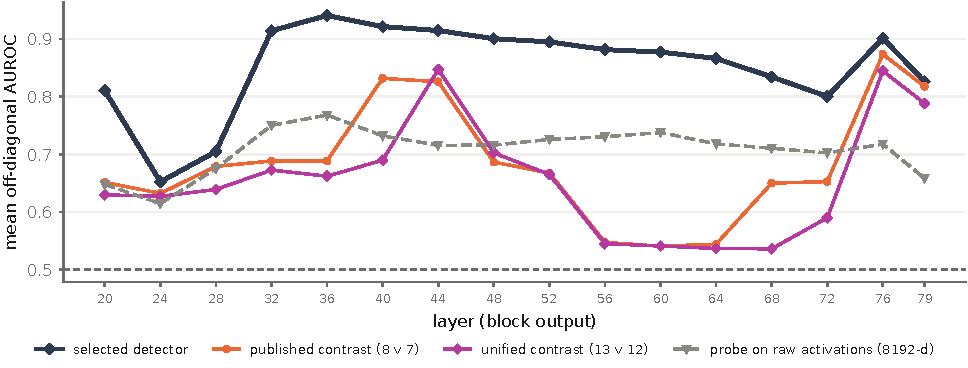
\includegraphics[width=\linewidth]{fig_selected_depth.pdf}
\caption{Transfer of the selected detector across the 16 layers against two persona contrasts and the
raw probe.}
\label{fig:selected-depth}
\end{figure}

\begin{table}[h]
\centering
\footnotesize
\caption{The knowledge direction, the extended contrast and the selected detector across depth.}
\label{tab:k-depth}
\resizebox{\linewidth}{!}{% Generated by make_thesis_assets.py
\begin{tabular}{@{}r ccc cc ccc@{}}
\toprule
 & \multicolumn{3}{c}{\hpkr, identical text} & \multicolumn{2}{c}{\hpkr, denials} & \multicolumn{3}{c}{Five-dataset mean} \\
\cmidrule(lr){2-4}\cmidrule(lr){5-6}\cmidrule(lr){7-9}
Layer & Knowledge direction & Knowledge direction, new questions & random & Knowledge direction & random & Knowledge direction & Extended contrast & Selected detector \\
\midrule
20 & 0.531 & 0.520 & 0.626 & 0.414 & 0.653 & 0.645 & 0.887 & 0.789 \\
24 & 0.652 & 0.646 & 0.649 & 0.477 & 0.669 & 0.600 & 0.865 & 0.739 \\
28 & 0.722 & 0.720 & 0.662 & 0.526 & 0.670 & 0.674 & 0.878 & 0.813 \\
32 & 0.783 & 0.779 & 0.702 & 0.607 & 0.691 & 0.791 & 0.905 & 0.898 \\
36 & 0.791 & 0.791 & 0.725 & 0.690 & 0.716 & 0.854 & 0.913 & 0.929 \\
40 & 0.793 & 0.796 & 0.734 & 0.728 & 0.728 & 0.825 & 0.899 & 0.906 \\
44 & 0.794 & 0.795 & 0.738 & 0.718 & 0.729 & 0.827 & 0.884 & 0.898 \\
48 & 0.794 & 0.795 & 0.738 & 0.710 & 0.729 & 0.816 & 0.865 & 0.882 \\
52 & 0.792 & 0.793 & 0.741 & 0.725 & 0.732 & 0.819 & 0.852 & 0.875 \\
56 & 0.792 & 0.793 & 0.734 & 0.728 & 0.719 & 0.812 & 0.831 & 0.860 \\
60 & 0.793 & 0.794 & 0.742 & 0.742 & 0.722 & 0.793 & 0.824 & 0.855 \\
64 & 0.793 & 0.793 & 0.733 & 0.731 & 0.726 & 0.756 & 0.826 & 0.843 \\
68 & 0.789 & 0.790 & 0.740 & 0.708 & 0.715 & 0.657 & 0.832 & 0.807 \\
72 & 0.786 & 0.788 & 0.739 & 0.722 & 0.728 & 0.637 & 0.818 & 0.774 \\
76 & 0.800 & 0.800 & 0.752 & 0.675 & 0.725 & 0.605 & 0.908 & 0.888 \\
79 & 0.823 & 0.822 & 0.760 & 0.794 & 0.733 & 0.789 & 0.831 & 0.854 \\
\bottomrule
\end{tabular}
}
\end{table}

\FloatBarrier
\section{The random persona bank}
\label{app:random}

\V{rb-roles} roles were drawn at random (one seed) from the Assistant Axis's 274 archetypes, built by
the bank pipeline with the same five variants, 30 questions, judge and filter, and partitioned into six
groups of the designed groups' sizes (8, 7, 5, 5, 4 and 6), giving random contrasts of the published
contrast's sizes (8 v 7) and of the extended contrast's (12 v 13), the second widening the first by four
and six random roles. Split 0 is the reported random bank; splits 1 to \V{rb-null-splits} are the
pre-registered null, and a test passes when its one-sided $p$ over them is at most 0.025. The six tests
were fixed before any direction was scored. \Cref{tab:random-bank} gives the null medians and 97.5th
percentiles from those splits and Holm-corrected $p$ values from \V{rb-holm-splits} further splits drawn by
the same rule.

\begin{table}[h]
\centering
\footnotesize
\caption{The random persona bank: six tests of the designed bank against the random null.}
\label{tab:random-bank}
\resizebox{\linewidth}{!}{% Generated by make_arxiv_assets.py from results/xmodel/llama/random_bank/s3/verdict.csv
\begin{tabular}{@{}l l c c c c l@{}}
\toprule
Test & Comparison & Designed bank & \shortstack{Null\\median} & \shortstack{Null\\97.5\%} & \shortstack{Holm\\$p$} & Verdict \\
\midrule
Transfer (off-diagonal AUROC) & extended contrast vs random 12 v 13 contrasts & 0.916 & 0.524 & 0.828 & 0.002 & pass \\
Zero-shot five-dataset mean & extended contrast vs random 12 v 13 contrasts & 0.899 & 0.609 & 0.814 & 0.002 & pass \\
Transfer with the knowledge direction & selected detector vs random contrast + knowledge direction & 0.922 & 0.812 & 0.891 & 0.002 & pass \\
HP-KR, all rows, AUROC & extended contrast vs random 12 v 13 contrasts & 0.912 & 0.648 & 0.938 & 0.144 & fail \\
Gain from widening, five-dataset mean & extended minus published contrast vs random 12 v 13 minus random 8 v 7 of the same split & $+$0.101 & $-$0.005 & $+$0.253 & 0.165 & fail \\
AISI held-out lies, AUROC & extended contrast vs random 12 v 13 contrasts & 0.977 & 0.804 & 0.955 & 0.002 & pass \\
\bottomrule
\end{tabular}
}
\end{table}

\FloatBarrier
\section{The knowledge direction}
\label{app:knowledge}

\Cref{fig:k-build} draws the construction. \Cref{tab:k-robust} gives the robustness checks (question
bootstrap, balanced splits, the replication with new questions), \cref{tab:k-paired} the paired
differences between the selected detector and the extended contrast on every set, \cref{tab:k-operating}
the share of lies caught at in-setting cutoffs, and \cref{tab:oracle} balanced accuracy under per-dataset
oracle thresholds. The 120 questions, the replication set and the template variants are in the
repository.

\begin{figure}[h]
\centering
\resizebox{\linewidth}{!}{% The knowledge direction's construction (copied by make_arxiv_assets.py from the thesis's
% fig_knowledge.tex). The same denial is written into the model's reply after a question it
% knows and after one nobody can know; the direction is the difference of the two means.
\ifdefined\thesisfigstyle\else% Shared style of the thesis's TikZ figures: the TeX Gyre Heros face (declared for XeTeX's TU
% encoding), the thesis palette and two drawing layers. Each figure file loads it once through
%   \ifdefined\thesisfigstyle\else\input{generated/fig_style}\fi
% make_thesis_assets.py copies it to generated/. Every line ends in % because figure files are read
% inside boxes, where a stray space would widen the figure.
\def\thesisfigstyle{}%
\newcommand{\figsf}{\sffamily}%
% palette: honest green and deceptive red are also the steering figure's colours
\definecolor{fhonest}{HTML}{1B8A5A}%
\definecolor{fhonestbg}{HTML}{DDF0E6}%
\definecolor{fdecept}{HTML}{C8423B}%
\definecolor{fdeceptbg}{HTML}{F7E0DE}%
\definecolor{famber}{HTML}{B7791F}%
\definecolor{fambersbg}{HTML}{F8EBD3}%
\definecolor{fslate}{HTML}{2E3A4F}%
\definecolor{fslatebg}{HTML}{E4E7EC}%
\definecolor{fcanvas}{HTML}{F4F2EE}%
\definecolor{fedge}{HTML}{D8D3CA}%
\definecolor{fink}{HTML}{1F2328}%
\definecolor{fmute}{HTML}{6B6B6B}%
\pgfdeclarelayer{figbase}%
\pgfdeclarelayer{figback}%
\pgfsetlayers{figbase,figback,main}%
\tikzset{
  fig/.style={x=1mm, y=1mm, font=\figsf\fontsize{6.6}{7.8}\selectfont, text=fink},
  figsmall/.style={font=\figsf\fontsize{5.9}{6.9}\selectfont},
  fighead/.style={font=\figsf\bfseries\fontsize{7.2}{8.4}\selectfont, text=fslate},
  figgloss/.style={font=\figsf\itshape\fontsize{6.1}{7.1}\selectfont, text=fmute},
  figpanel/.style={draw=fedge, fill=white, rounded corners=2.2mm, line width=0.4pt},
  figarrow/.style={-{Stealth[length=1.6mm, width=1.2mm]}, line width=0.6pt},
}%
\fi%
\begin{tikzpicture}[fig,
    qbox/.style={figpanel, align=left, text width=#1, inner sep=1.5mm,
                 font=\figsf\fontsize{6.3}{7.6}\selectfont},
    reply/.style={rounded corners=1.4mm, inner sep=1.4mm, line width=0.5pt,
                  font=\figsf\fontsize{6.5}{7.6}\selectfont},
    eqchip/.style={draw=fslate!40, fill=white, rounded corners=1.2mm, inner sep=1.6mm,
                   font=\figsf\fontsize{6.8}{8}\selectfont}]
\fill[fcanvas, rounded corners=3mm] (0,0) rectangle (150,64);
% ---- the two kinds of question --------------------------------------------------------------
\node[fighead, anchor=west] at (5,58) {The model knows the answer \textmd{\textit{(60 questions)}}};
\node[fighead, anchor=west] at (5,29.5) {Nobody can know the answer \textmd{\textit{(60 questions)}}};
\node[qbox=50mm, anchor=north west] (q1) at (5,53.5)
  {What is the capital city of France?\\
   A.\,Lyon \quad B.\,Marseille \quad C.\,Paris \quad D.\,Nice\\[0.4ex]
   \textit{Tell me whether you know the answer to the question.}};
\node[qbox=50mm, anchor=north west] (q2) at (5,25)
  {How many paper cups were used in the staff kitchen of the Lisbon city library on
   14 March 2019?\\[0.4ex]
   \textit{Tell me whether you know the answer to the question.}};
% ---- the same reply, written for the model ------------------------------------------------------
\node[reply, fill=fdeceptbg, draw=fdecept, anchor=west] (r1) at (64,44) {``I do not know the answer.''};
\node[reply, fill=fhonestbg, draw=fhonest, anchor=west] (r2) at (64,15.5) {``I do not know the answer.''};
\node[figgloss, anchor=north, text=fdecept] at ($(r1.south)+(0,-0.8)$) {false for this model};
\node[figgloss, anchor=north, text=fhonest] at ($(r2.south)+(0,-0.8)$) {true for this model};
\draw[figarrow, fmute] (q1.east |- r1.west) -- (r1.west);
\draw[figarrow, fmute] (q2.east |- r2.west) -- (r2.west);
% ---- mean activation over the reply's tokens ------------------------------------------------------
\foreach \y/\c in {44/fdecept, 15.5/fhonest} {
  \foreach \i/\s in {0/60, 1/25, 2/80, 3/40, 4/15, 5/65} {
    \fill[\c!\s] (102,\y+4.2-\i*1.7) rectangle ++(2.6,1.5);}
  \draw[fedge, line width=0.3pt] (102,\y-4.3) rectangle (104.6,\y+5.7);}
\node[figsmall, anchor=south, text=fdecept] at (103.3,50.4) {$\bar h_{\text{knows}}$};
\node[figsmall, anchor=north, text=fhonest] at (103.3,10.4) {$\bar h_{\text{cannot}}$};
\draw[figarrow, fmute] (r1.east) -- (101,44);
\draw[figarrow, fmute] (r2.east) -- (101,15.5);
\node[figgloss, align=center] at (103.3,30) {layer 40,\\mean over\\the reply};
% ---- the direction ------------------------------------------------------------------------------
\node[eqchip, anchor=west] (k) at (111.5,30)
  {$\hat v_{\mathrm{know}}=\operatorname{unit}\bigl(\bar h_{\text{knows}}-\bar h_{\text{cannot}}\bigr)$};
\draw[figarrow, fslate!70] (105.2,44) to[out=0, in=100] (k.north);
\draw[figarrow, fslate!70] (105.2,15.5) to[out=0, in=260] (k.south);
\end{tikzpicture}%
}
\caption{The knowledge direction: the same denial after known and after unknowable questions.}
\label{fig:k-build}
\end{figure}

\begin{table}[h]
\centering
\footnotesize
\caption{Robustness of the knowledge direction on \hpkr's identical text.}
\label{tab:k-robust}
\resizebox{\linewidth}{!}{% Generated by make_thesis_assets.py
\begin{tabular}{@{}l l ccc@{}}
\toprule
Set & Check & Layer 36 & Layer 40 & Layer 44 \\
\midrule
\hpkr, identical text & AUROC [question bootstrap] & 0.791 [0.790, 0.792] & 0.793 [0.792, 0.794] & 0.794 [0.793, 0.795] \\
 & random directions, 97.5th pct. & 0.732 & 0.736 & 0.733 \\
 & share of balanced splits as high & 0.000 & 0.000 & 0.000 \\
 & new questions (knowledge direction, new questions) & 0.791 & 0.796 & 0.795 \\
\addlinespace
\hpkr, denials & AUROC [question bootstrap] & 0.690 [0.684, 0.697] & 0.728 [0.723, 0.733] & 0.718 [0.713, 0.724] \\
 & random directions, 97.5th pct. & 0.717 & 0.730 & 0.724 \\
 & share of balanced splits as high & 0.072 & 0.042 & 0.055 \\
 & new questions (knowledge direction, new questions) & 0.686 & 0.729 & 0.718 \\
\addlinespace
Gender-Secret (fine-tune read) & AUROC [question bootstrap] & 0.810 [0.804, 0.817] & 0.865 [0.860, 0.870] & 0.869 [0.864, 0.873] \\
 & random directions, 97.5th pct. & 0.814 & 0.817 & 0.856 \\
 & share of balanced splits as high & 0.042 & 0.014 & 0.015 \\
 & new questions (knowledge direction, new questions) & 0.836 & 0.881 & 0.878 \\
\addlinespace
All & $\cos(\mathrm{knowledge direction}', \mathrm{knowledge direction})$ & 0.99 & 0.99 & 0.99 \\
\bottomrule
\end{tabular}
}
\end{table}

\begin{table}[h]
\centering
\footnotesize
\caption{Paired differences, selected detector minus extended contrast, with 95\% intervals.}
\label{tab:k-paired}
\resizebox{\linewidth}{!}{% Generated by make_thesis_assets.py from k_robustness.py paired
\begin{tabular}{@{}l ccc@{}}
\toprule
Comparison & Five-dataset mean & \hpkr, identical text & \hpkr, denials \\
\midrule
Selected detector $-$ extended contrast & $+$0.007 [$-$0.004, $+$0.018] & $+$0.066 [$+$0.037, $+$0.098] & $+$0.054 [$+$0.025, $+$0.082] \\
Selected detector $-$ knowledge-denial contrast & $+$0.012 [$+$0.001, $+$0.023] & $+$0.075 [$+$0.040, $+$0.112] & $+$0.154 [$+$0.112, $+$0.196] \\
Selected detector $-$ knowledge direction & $+$0.082 [$+$0.073, $+$0.091] & $-$0.006 [$-$0.014, $+$0.002] & $-$0.004 [$-$0.011, $+$0.003] \\
Selected detector $-$ base probe, layer 40 & $+$0.128 [$+$0.112, $+$0.145] & $+$0.008 [$-$0.023, $+$0.035] & $+$0.131 [$+$0.088, $+$0.178] \\
Published contrast + knowledge direction $-$ published contrast & $+$0.081 [$+$0.068, $+$0.096] & $+$0.074 [$+$0.040, $+$0.111] & $+$0.072 [$+$0.037, $+$0.104] \\
\bottomrule
\end{tabular}
}
\end{table}

\begin{table}[h]
\centering
\footnotesize
\caption{Share of lies caught at cutoffs set on each dataset's own honest answers, layer 40.}
\label{tab:k-operating}
\resizebox{\linewidth}{!}{% Generated by make_thesis_assets.py
\begin{tabular}{@{}l ccc cc@{}}
\toprule
 & \multicolumn{3}{c}{In-setting cutoff: lies caught} & \multicolumn{2}{c}{Alpaca 1\% threshold} \\
\cmidrule(lr){2-4}\cmidrule(lr){5-6}
Detector & 1\% & 5\% & 10\% & lies caught & honest flagged \\
\midrule
Base probe, layer 40 & 0.32 & 0.53 & 0.66 & 0.28 & 0.03 \\
Published contrast & 0.34 & 0.49 & 0.58 & 0.38 & 0.03 \\
Published contrast + knowledge direction & 0.32 & 0.55 & 0.67 & 0.41 & 0.12 \\
Extended contrast & 0.47 & 0.68 & 0.77 & 0.41 & 0.03 \\
Knowledge direction & 0.21 & 0.42 & 0.56 & 0.34 & 0.23 \\
Selected detector & 0.38 & 0.63 & 0.73 & 0.47 & 0.07 \\
\bottomrule
\end{tabular}
}
\end{table}

\begin{table}[h]
\centering
\footnotesize
\caption{Balanced accuracy at the Alpaca threshold and under per-dataset oracle thresholds.}
\label{tab:oracle}
\resizebox{\linewidth}{!}{% Generated by make_thesis_assets.py
\begin{tabular}{@{}l cccc@{}}
\toprule
 & \multicolumn{2}{c}{Layer 36} & \multicolumn{2}{c}{Layer 40} \\
\cmidrule(lr){2-3}\cmidrule(lr){4-5}
Detector & Alpaca & oracle & Alpaca & oracle \\
\midrule
Base probe (RepE) & 0.650 & 0.635 & 0.626 & 0.652 \\
Knowledge-denial (knowledge-denial contrast) & 0.695 & 0.675 & 0.725 & 0.692 \\
Extended (extended contrast) & 0.712 & 0.710 & 0.694 & 0.718 \\
\bottomrule
\end{tabular}
}
\end{table}

\begin{table}[h]
\centering
\footnotesize
\caption{Balanced accuracy at the benchmark's threshold for every detector and dataset.}
\label{tab:operating}
\resizebox{\linewidth}{!}{% Generated by make_numbers.py
\begin{tabular}{llccc}
\toprule
Layer & Detector & Balanced acc. & Recall & AUROC \\
\midrule
\multirow{4}{*}{L20} & Base probe (trained on RepE) & 0.721 & 0.489 & 0.697 \\
 & Published contrast (8 v 7) & 0.534 & 0.069 & 0.750 \\
 & Knowledge-denial contrast (4 v 6) & 0.559 & 0.305 & 0.863 \\
 & Extended contrast (12 v 13) & 0.591 & 0.187 & 0.887 \\
\midrule
\multirow{4}{*}{L40} & Base probe (trained on RepE) & 0.626 & 0.281 & 0.778 \\
 & Published contrast (8 v 7) & 0.675 & 0.382 & 0.798 \\
 & Knowledge-denial contrast (4 v 6) & 0.725 & 0.487 & 0.894 \\
 & Extended contrast (12 v 13) & 0.694 & 0.413 & 0.899 \\
\midrule
\multirow{4}{*}{L44} & Base probe (trained on RepE) & 0.626 & 0.281 & 0.756 \\
 & Published contrast (8 v 7) & 0.654 & 0.318 & 0.791 \\
 & Knowledge-denial contrast (4 v 6) & 0.683 & 0.395 & 0.880 \\
 & Extended contrast (12 v 13) & 0.666 & 0.350 & 0.884 \\
\bottomrule
\end{tabular}}
\end{table}

\FloatBarrier
\section{Model organisms}
\label{app:organisms}

\Cref{fig:k-gs} shows Gender-Secret at layers 36 and 40, each detector on the fine-tune's read and on the
base model's read of the same transcripts, directions built inside the model read. \Cref{tab:xm-organisms}
gives every fine-tune of the three further models, with the base model's read beside the fine-tune's. On
Llama's two Soft-Trigger fine-tunes the knowledge direction clears the fine-tune read's band at layer~40
(greeting \V{th-k-st-greeting-ft-kft-L40} against \V{th-k-st-greeting-ft-band-L40}, time
\V{th-k-st-time-ft-kft-L40} against \V{th-k-st-time-ft-band-L40}), but the base model's read of the same
transcripts does too (greeting \V{th-k-st-greeting-base-kft-L40} against
\V{th-k-st-greeting-base-band-L40}, time \V{th-k-st-time-base-kft-L40} against
\V{th-k-st-time-base-band-L40}): the trigger can be read from the text, so these organisms cannot credit a
detector of the fine-tune's state, and the same holds for Mistral's.

\begin{figure}[h]
\centering
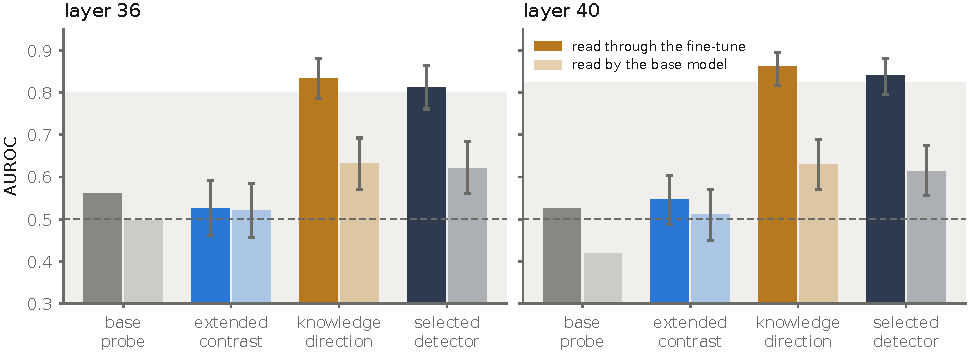
\includegraphics[width=\linewidth]{fig_knowledge_gs.pdf}
\caption{Gender-Secret read through the fine-tune (dark) and by the base model (light); grey marks the
central 95\% of random directions.}
\label{fig:k-gs}
\end{figure}

\begin{table}[h]
\centering
\footnotesize
\caption{The fine-tunes of the three further models: AUROC on the fine-tune's read and on the base
model's read of the same transcripts.}
\label{tab:xm-organisms}
\resizebox{\linewidth}{!}{% Generated by make_xmodel_assets.py from organisms.py score
\begin{tabular}{@{}ll cccc c cc@{}}
\toprule
 & & \multicolumn{5}{c}{The fine-tune's read} & \multicolumn{2}{c}{The base model's read} \\
\cmidrule(lr){3-7}\cmidrule(lr){8-9}
Model & Fine-tune & \shortstack{Extended\\contrast} & \shortstack{Knowledge\\direction} & \shortstack{Selected\\detector} & Probe & Band & \shortstack{Knowledge\\direction} & Band \\
\midrule
Qwen$^\dagger$ & Soft-Trigger, greeting & 0.455 & 0.469 & 0.456 & 0.708 & 0.691 & 0.430 & 0.669 \\
 & Soft-Trigger, time & 0.569 & 0.531 & 0.544 & 0.654 & 0.710 & 0.451 & 0.700 \\
 & Soft-Trigger, gender & 0.479 & 0.454 & 0.452 & 0.680 & 0.734 & 0.444 & 0.660 \\
\addlinespace
Mistral & Gender-Secret & 0.406 & 0.440 & 0.414 & 0.400 & 0.765 & 0.497 & 0.784 \\
 & Soft-Trigger, greeting & 0.931 & 0.930 & 0.936 & 0.878 & 0.900 & 0.872 & 0.823 \\
 & Soft-Trigger, time & 0.929 & 0.946 & 0.949 & 0.275 & 0.930 & 0.875 & 0.858 \\
 & Soft-Trigger, gender & 0.948 & 0.935 & 0.940 & 0.901 & 0.892 & 0.873 & 0.828 \\
\addlinespace
Gemma & Soft-Trigger, greeting & 0.101 & 0.290 & 0.164 & 0.845 & 0.933 & 0.839 & 0.858 \\
 & Soft-Trigger, time & 0.916 & 0.719 & 0.876 & 1.000 & 0.962 & 0.860 & 0.875 \\
 & Soft-Trigger, gender & 0.560 & 0.804 & 0.763 & 0.794 & 0.951 & 0.849 & 0.868 \\
\bottomrule
\end{tabular}
}
\end{table}

\FloatBarrier
\section{Steering}
\label{app:steering}

\Cref{tab:steering} gives disclosure of the hidden fact under each direction at $c = \pm 0.3$ over the
\V{th-steer-n} scenarios, with paired changes and 95\% intervals. For each scenario the eleven answers
(unsteered, and five directions at both signs) were shuffled with their conditions hidden and labelled by
one reader, an AI assistant, before the key was opened; the labels are not those of a validated grader.

Two small runs steered the knowledge direction with an absolute shift at the same block (figures quoted
from their reports). On \hpkr{} questions, subtracting it made the model deny knowing answers it still gave
on the answer check (denials rising from 0.05 to 0.70 without pressure at $\alpha = -4$, and to 17 of 20 by
hand at $-8$, against a rise of at most 0.10 for random directions of the same size at $\pm 4$), adding it
produced no usable effect, and general-knowledge items did not move; this run was graded by pattern
matching with every answer also read by hand. On the Gender-Secret fine-tune, read by hand without
blinding, the knowledge direction rebuilt inside the fine-tune, at either sign, revealed the hidden gender
more often than one random direction at every matched size, but every reveal under any push
fell on a prompt with an earlier male-coded turn, and the belief the fine-tune holds did not move; with one
random direction and 20 items per condition the excess is suggestive only.

\begin{table}[h]
\centering
\footnotesize
\caption{Disclosure of the hidden fact under steering at $c=\pm0.3$: one blinded reader's labels of
\V{th-steer-n} scenarios, one greedy answer each.}
\label{tab:steering}
\resizebox{\linewidth}{!}{\begin{tabular}{lcccc}
\toprule
 & \multicolumn{2}{c}{honest side ($c=-0.3$)} & \multicolumn{2}{c}{deceptive side ($c=+0.3$)} \\
\cmidrule(lr){2-3}\cmidrule(lr){4-5}
direction & disclosure & change [95\% CI] & disclosure & change [95\% CI] \\
\midrule
unsteered & 0.48 & -- & 0.48 & -- \\
Extended contrast (12 v 13) & 0.61 & $+0.13$ [0.00, $+0.26$] & 0.20 & {\boldmath$-0.28$} [$-0.41$, $-0.13$] \\
Published contrast (8 v 7) & 0.57 & $+0.09$ [$-0.06$, $+0.24$] & 0.20 & {\boldmath$-0.28$} [$-0.41$, $-0.15$] \\
Base probe (trained on RepE) & 0.50 & $+0.02$ [$-0.11$, $+0.15$] & 0.39 & $-0.09$ [$-0.22$, $+0.04$] \\
random direction 1 & 0.43 & $-0.06$ [$-0.17$, $+0.04$] & 0.48 & 0.00 [$-0.09$, $+0.09$] \\
random direction 2 & 0.46 & $-0.02$ [$-0.09$, $+0.06$] & 0.52 & $+0.04$ [$-0.11$, $+0.19$] \\
\bottomrule
\end{tabular}
}
\end{table}

\FloatBarrier
\section{The four models}
\label{app:models}

\Cref{tab:models} lists the four models, \cref{fig:xm-depth} follows four measures over each model's
depth sweep, \cref{tab:xm-mid} gives the
main detectors at each model's middle block, \cref{tab:xm-intervals} the paired intervals behind
\cref{tab:claims}, \cref{tab:xm-zeroshot} every contrast on every dataset,
\cref{tab:xm-transfer} transfer for every feature set, \cref{tab:xm-wording} the wording-controlled
slices, \cref{tab:xm-operating} the tail, \cref{tab:xm-aisi} the probe trained on the model's own lies
where those exist (Llama and Gemma), and \cref{tab:xm-checks} the template-free knowledge direction and
the token reads.

\begin{table}[h]
\centering
\footnotesize
\caption{The four models: blocks and width, the block read for each of Llama's layers, the datasets the
benchmark gives each, the judge score a rollout needs to enter the bank, and the share of rollouts
scored fully in role.}
\label{tab:models}
\resizebox{\linewidth}{!}{% Generated by make_xmodel_assets.py from lb_models.SPECS and the judge's scores
\begin{tabular}{@{}l cc ccc l l c@{}}
\toprule
 & & & \multicolumn{3}{c}{Block read for Llama's layer} & & & \\
\cmidrule(lr){4-6}
Model & Blocks & Width & 20 & 40 & 36, 44 & Liars' Bench datasets & Bank & In role \\
\midrule
Llama-3.3-70B & 80 & 8192 & 20 & 40 & 36, 44 & CG, \hpc, \hpkr, IT, ID & score 3 & 69\% \\
Qwen2.5-72B$^\dagger$ & 80 & 8192 & 20 & 40 & 36, 44 & \hpc, \hpkr, ID & score 2--3 & 28\% \\
Mistral-Small-3.1-24B & 40 & 5120 & 9 & 20 & 18, 22 & \hpc, \hpkr, IT, ID & score 3 & 68\% \\
Gemma-3-27B & 62 & 5376 & 8 & 31 & 28, 34 & CG, IT, ID & score 3 & 96\% \\
\bottomrule
\end{tabular}
}
\end{table}

\begin{figure}[h]
\centering
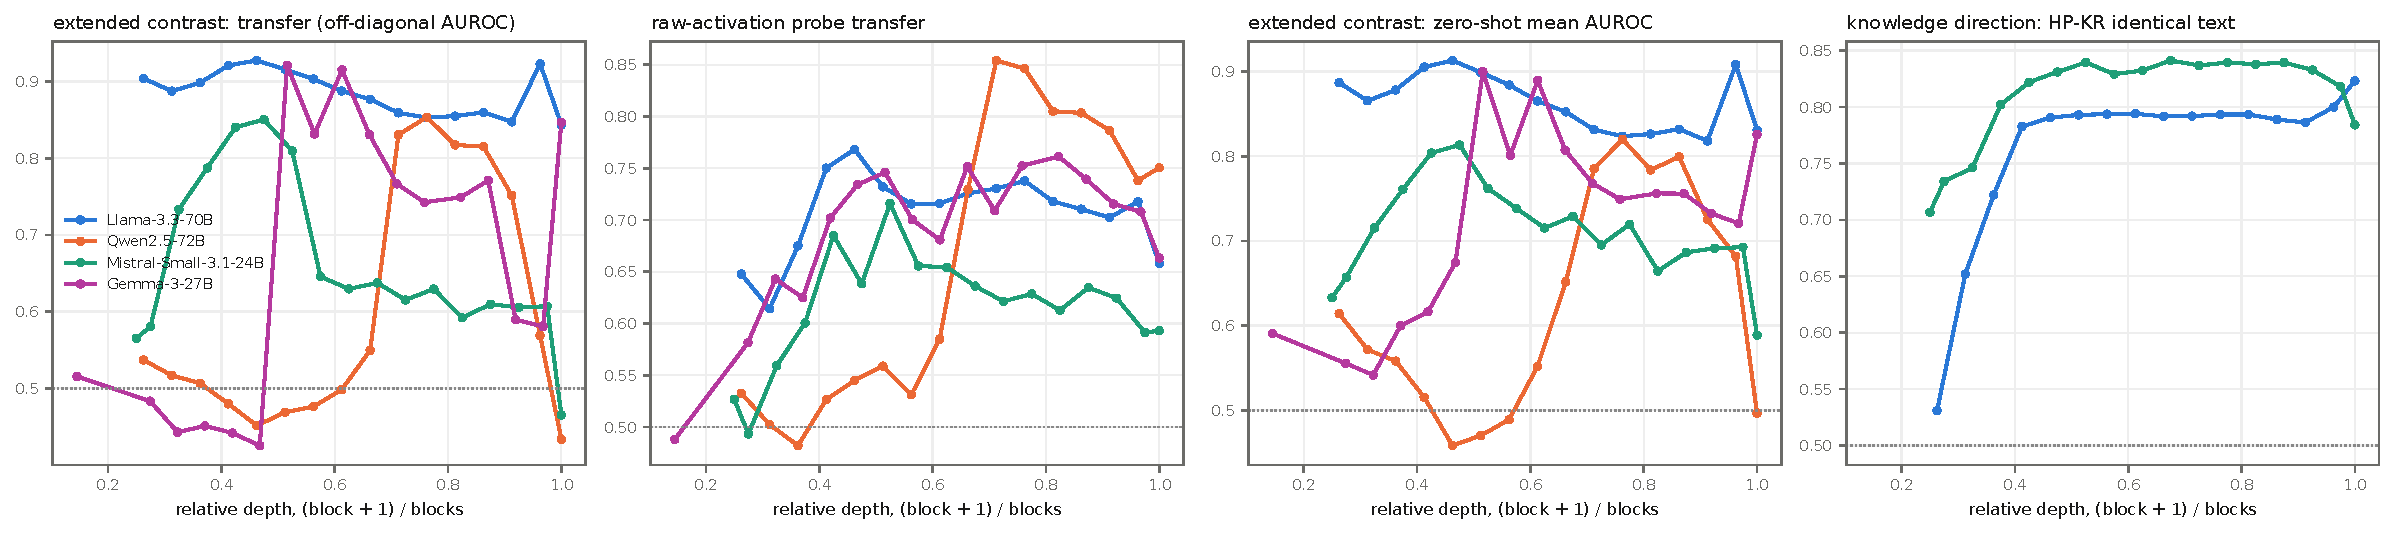
\includegraphics[width=\linewidth]{fig_xmodel_depth.pdf}
\caption{Four measures over each model's 16-depth sweep, by relative depth; the last panel has the two
models with a released identical-text slice.}
\label{fig:xm-depth}
\end{figure}

\begin{table}[h]
\centering
\footnotesize
\caption{The main detectors at each model's middle block.}
\label{tab:xm-mid}
% Generated by make_xmodel_assets.py from the persona_ood, recall_denial and k_robustness outputs
\begin{tabular}{@{}l cccc@{}}
\toprule
 & Llama & Qwen$^\dagger$ & Mistral & Gemma \\
\midrule
\multicolumn{5}{@{}l}{\emph{Transfer, mean off-diagonal AUROC}} \\
Probe on raw activations & 0.732 & 0.559 & 0.716 & 0.746 \\
Published contrast & 0.832 & 0.451 & 0.633 & 0.700 \\
Knowledge-denial contrast & 0.912 & 0.679 & 0.780 & 0.442 \\
Extended contrast & 0.916 & 0.453 & 0.810 & 0.921 \\
Knowledge direction & 0.823 & 0.508 & 0.799 & 0.457 \\
Selected detector & 0.922 & 0.514 & 0.841 & 0.860 \\
\midrule
\multicolumn{5}{@{}l}{\emph{Zero-shot, mean AUROC over the model's datasets}} \\
Mean Probe (Liars' Bench, published) & 0.682 & 0.530 & 0.570 & 0.527 \\
Base probe, same block & 0.778 & 0.498 & 0.766 & 0.783 \\
Published contrast & 0.798 & 0.380 & 0.719 & 0.679 \\
Knowledge-denial contrast & 0.894 & 0.668 & 0.727 & 0.484 \\
Extended contrast & 0.899 & 0.441 & 0.762 & 0.900 \\
Knowledge direction & 0.825 & 0.546 & 0.775 & 0.515 \\
Selected detector & 0.906 & 0.533 & 0.804 & 0.847 \\
\midrule
\multicolumn{5}{@{}l}{\emph{Lies caught at 1\% of honest answers flagged}} \\
Extended contrast & 0.47 & 0.02 & 0.14 & 0.43 \\
Selected detector & 0.38 & 0.03 & 0.23 & 0.30 \\
\bottomrule
\end{tabular}

\end{table}

\begin{table}[h]
\centering
\footnotesize
\caption{Paired differences at each model's middle block, with 95\% intervals.}
\label{tab:xm-intervals}
\resizebox{\linewidth}{!}{% Generated by make_xmodel_assets.py from transfer_ci.py and k_robustness.py paired
\begin{tabular}{@{}ll cccc@{}}
\toprule
& Comparison & Llama & Qwen$^\dagger$ & Mistral & Gemma \\
\midrule
Transfer & Extended contrast $-$ raw probe & $+$0.184 [$+$0.172, $+$0.195] & $-$0.106 [$-$0.116, $-$0.094] & $+$0.094 [$+$0.082, $+$0.105] & $+$0.175 [$+$0.166, $+$0.184] \\
Transfer & Extended contrast $-$ published contrast & $+$0.084 [$+$0.074, $+$0.094] & $+$0.002 [$-$0.007, $+$0.012] & $+$0.176 [$+$0.169, $+$0.183] & $+$0.221 [$+$0.203, $+$0.238] \\
Transfer & Selected detector $-$ raw probe & $+$0.190 [$+$0.179, $+$0.199] & $-$0.045 [$-$0.057, $-$0.032] & $+$0.125 [$+$0.115, $+$0.136] & $+$0.114 [$+$0.101, $+$0.125] \\
Transfer & Selected detector $-$ extended contrast & $+$0.006 [$-$0.003, $+$0.015] & $+$0.060 [$+$0.052, $+$0.069] & $+$0.032 [$+$0.021, $+$0.043] & $-$0.061 [$-$0.069, $-$0.055] \\
Transfer & Published contrast + knowledge direction $-$ published contrast & $+$0.067 [$+$0.055, $+$0.078] & $+$0.052 [$+$0.040, $+$0.064] & $+$0.202 [$+$0.192, $+$0.213] & $+$0.110 [$+$0.098, $+$0.124] \\
Mean & Extended contrast $-$ published contrast & $+$0.101 [$+$0.089, $+$0.112] & $+$0.061 [$+$0.055, $+$0.067] & $+$0.043 [$+$0.034, $+$0.052] & $+$0.221 [$+$0.201, $+$0.240] \\
Mean & Selected detector $-$ extended contrast & $+$0.007 [$-$0.004, $+$0.018] & $+$0.093 [$+$0.078, $+$0.107] & $+$0.042 [$+$0.028, $+$0.056] & $-$0.053 [$-$0.057, $-$0.049] \\
Mean & Selected detector $-$ RepE probe & $+$0.128 [$+$0.112, $+$0.145] & $+$0.036 [$+$0.016, $+$0.057] & $+$0.038 [$+$0.022, $+$0.053] & $+$0.064 [$+$0.050, $+$0.078] \\
\bottomrule
\end{tabular}
}
\end{table}

\begin{table}[h]
\centering
\footnotesize
\caption{Zero-shot AUROC per dataset at each model's middle block.}
\label{tab:xm-zeroshot}
\resizebox{\linewidth}{!}{% Generated by make_xmodel_assets.py from persona_ood zero_shot.csv
\begin{tabular}{@{}ll cccccc c@{}}
\toprule
Model & Contrast & CG & \hpc & \hpkr & IT & ID & RepE & Mean \\
\midrule
Llama & Published contrast & 0.865 & 0.581 & 0.593 & 0.979 & 0.974 & 1.000 & 0.798 \\
 & Knowledge-denial contrast & 0.902 & 0.755 & 0.919 & 0.913 & 0.980 & 1.000 & 0.894 \\
 & Extended contrast & 0.912 & 0.712 & 0.912 & 0.980 & 0.978 & 1.000 & 0.899 \\
\addlinespace
Qwen$^\dagger$ & Published contrast & n/a & 0.512 & 0.094 & n/a & 0.534 & 0.700 & 0.380 \\
 & Knowledge-denial contrast & n/a & 0.573 & 0.783 & n/a & 0.648 & 0.711 & 0.668 \\
 & Extended contrast & n/a & 0.539 & 0.187 & n/a & 0.597 & 0.744 & 0.441 \\
\addlinespace
Mistral & Published contrast & n/a & 0.456 & 0.758 & 0.729 & 0.934 & 1.000 & 0.719 \\
 & Knowledge-denial contrast & n/a & 0.716 & 0.712 & 0.542 & 0.937 & 0.995 & 0.727 \\
 & Extended contrast & n/a & 0.606 & 0.793 & 0.708 & 0.941 & 1.000 & 0.762 \\
\addlinespace
Gemma & Published contrast & 0.613 & n/a & n/a & 0.544 & 0.881 & 0.762 & 0.679 \\
 & Knowledge-denial contrast & 0.641 & n/a & n/a & 0.603 & 0.209 & 0.344 & 0.484 \\
 & Extended contrast & 0.819 & n/a & n/a & 0.930 & 0.951 & 0.985 & 0.900 \\
\bottomrule
\end{tabular}
}
\end{table}

\begin{table}[h]
\centering
\footnotesize
\caption{Transfer (mean off-diagonal AUROC) at each model's middle block.}
\label{tab:xm-transfer}
\resizebox{\linewidth}{!}{% Generated by make_xmodel_assets.py from persona_ood summary.csv and recall_denial transfer
\begin{tabular}{@{}l cc cccccc ccc@{}}
\toprule
 & & & & & & & & & \multicolumn{3}{c}{Probe on $k = 3$} \\
\cmidrule(lr){10-12}
Model & Layer & Block & Raw & \shortstack{Published\\contrast} & \shortstack{Knowledge-\\denial contrast} & \shortstack{Extended\\contrast} & \shortstack{Knowledge\\direction} & \shortstack{Selected\\detector} & Published & Extended & Random \\
\midrule
Llama & 20 & 20 & 0.648 & 0.651 & 0.866 & 0.904 & 0.574 & 0.811 & 0.679 & 0.684 & 0.527 \\
 & 36$^*$ & 36 & 0.768 & 0.689 & 0.912 & 0.927 & 0.854 & 0.941 & 0.679 & 0.879 & 0.481 \\
 & 40 & 40 & 0.732 & 0.832 & 0.912 & 0.916 & 0.823 & 0.922 & 0.639 & 0.866 & 0.504 \\
 & 44$^*$ & 44 & 0.716 & 0.826 & 0.900 & 0.903 & 0.832 & 0.915 & 0.617 & 0.880 & 0.493 \\
\addlinespace
Qwen$^\dagger$ & 20 & 20 & 0.533 & 0.468 & 0.560 & 0.525 & 0.460 & 0.533 & 0.594 & 0.674 & 0.516 \\
 & 36$^*$ & 36 & 0.545 & 0.407 & 0.620 & 0.425 & 0.523 & 0.528 & 0.521 & 0.578 & 0.488 \\
 & 40 & 40 & 0.559 & 0.451 & 0.679 & 0.453 & 0.508 & 0.514 & 0.476 & 0.539 & 0.491 \\
 & 44$^*$ & 44 & 0.531 & 0.426 & 0.701 & 0.478 & 0.504 & 0.518 & 0.487 & 0.554 & 0.486 \\
\addlinespace
Mistral & 20 & 9 & 0.527 & 0.483 & 0.559 & 0.565 & 0.466 & 0.544 & 0.522 & 0.559 & 0.487 \\
 & 36$^*$ & 18 & 0.638 & 0.821 & 0.811 & 0.850 & 0.775 & 0.860 & 0.786 & 0.848 & 0.526 \\
 & 40 & 20 & 0.716 & 0.633 & 0.780 & 0.810 & 0.799 & 0.841 & 0.760 & 0.704 & 0.554 \\
 & 44$^*$ & 22 & 0.656 & 0.619 & 0.771 & 0.646 & 0.834 & 0.863 & 0.742 & 0.741 & 0.527 \\
\addlinespace
Gemma & 20 & 8 & 0.488 & 0.510 & 0.526 & 0.515 & 0.509 & 0.457 & 0.506 & 0.532 & 0.488 \\
 & 36$^*$ & 28 & 0.734 & 0.428 & 0.422 & 0.425 & 0.419 & 0.421 & 0.767 & 0.845 & 0.493 \\
 & 40 & 31 & 0.746 & 0.700 & 0.442 & 0.921 & 0.457 & 0.860 & 0.863 & 0.874 & 0.558 \\
 & 44$^*$ & 34 & 0.700 & 0.719 & 0.440 & 0.832 & 0.801 & 0.866 & 0.855 & 0.860 & 0.511 \\
\bottomrule
\end{tabular}
}
\end{table}

\begin{table}[h]
\centering
\footnotesize
\caption{\hpkr's wording-controlled slices on every model that has them.}
\label{tab:xm-wording}
\resizebox{\linewidth}{!}{% Generated by make_xmodel_assets.py from recall_denial.py combine and k_models.py hpkr_score
\begin{tabular}{@{}ll cc c ccccc c@{}}
\toprule
Model & Slice & Lies & Honest & Probe & \shortstack{Published\\contrast} & \shortstack{Knowledge-\\denial contrast} & \shortstack{Extended\\contrast} & \shortstack{Knowledge\\direction} & \shortstack{Selected\\detector} & Band \\
\midrule
Llama & Identical text & 78 & 112 & 0.779 & 0.715 & 0.712 & 0.721 & 0.793 & 0.787 & 0.733 \\
 & Denials & 125 & 135 & 0.593 & 0.649 & 0.570 & 0.670 & 0.728 & 0.724 & 0.726 \\
Mistral & Identical text & 494 & 729 & 0.766 & 0.784 & 0.647 & 0.760 & 0.840 & 0.840 & 0.755 \\
 & Denials & 677 & 1,020 & 0.758 & 0.763 & 0.571 & 0.701 & 0.835 & 0.832 & 0.748 \\
Qwen$^\dagger$ & Denials & 539 & 44 & 0.566 & 0.495 & 0.580 & 0.509 & 0.632 & 0.622 & 0.622 \\
 & Identical reply, rebuilt & 435 & 128 & 0.543 & 0.504 & 0.550 & 0.518 & 0.602 & 0.598 & 0.584 \\
 & Denials, rebuilt & 571 & 164 & 0.533 & 0.498 & 0.569 & 0.547 & 0.613 & 0.617 & 0.580 \\
Gemma & Opening sentence, rebuilt & 34 & 85 & 0.481 & 0.484 & 0.530 & 0.624 & 0.585 & 0.611 & 0.622 \\
 & Denials, rebuilt & 35 & 100 & 0.547 & 0.583 & 0.418 & 0.434 & 0.378 & 0.403 & 0.637 \\
\bottomrule
\end{tabular}
}
\end{table}

\begin{table}[h]
\centering
\footnotesize
\caption{Share of lies caught at in-setting cutoffs, each model's middle block.}
\label{tab:xm-operating}
\resizebox{\linewidth}{!}{% Generated by make_xmodel_assets.py from k_robustness.py operating points
\begin{tabular}{@{}l cc cc cc cc@{}}
\toprule
 & \multicolumn{2}{c}{Llama} & \multicolumn{2}{c}{Qwen$^\dagger$} & \multicolumn{2}{c}{Mistral} & \multicolumn{2}{c}{Gemma} \\
\cmidrule(lr){2-3}\cmidrule(lr){4-5}\cmidrule(lr){6-7}\cmidrule(lr){8-9}
Detector & 1\% & 10\% & 1\% & 10\% & 1\% & 10\% & 1\% & 10\% \\
\midrule
Base probe & 0.32 & 0.66 & 0.02 & 0.17 & 0.13 & 0.47 & 0.28 & 0.66 \\
Published contrast & 0.34 & 0.58 & 0.02 & 0.12 & 0.13 & 0.47 & 0.08 & 0.30 \\
Extended contrast & 0.47 & 0.77 & 0.02 & 0.14 & 0.14 & 0.49 & 0.43 & 0.78 \\
Knowledge direction & 0.21 & 0.56 & 0.02 & 0.13 & 0.21 & 0.54 & 0.07 & 0.26 \\
Selected detector & 0.38 & 0.73 & 0.03 & 0.13 & 0.23 & 0.59 & 0.30 & 0.63 \\
Published contrast + knowledge direction & 0.32 & 0.67 & 0.02 & 0.11 & 0.22 & 0.59 & 0.24 & 0.53 \\
\bottomrule
\end{tabular}
}
\end{table}

\begin{table}[h]
\centering
\footnotesize
\caption{The probe trained on the model's own belief-labelled lies, Llama and Gemma.}
\label{tab:xm-aisi}
\resizebox{\linewidth}{!}{% Generated by make_xmodel_assets.py from aisi_probe.py compare
\begin{tabular}{@{}l ccc ccc@{}}
\toprule
 & \multicolumn{3}{c}{Llama} & \multicolumn{3}{c}{Gemma} \\
\cmidrule(lr){2-4}\cmidrule(lr){5-7}
Detector, at the block for layer & 20 & 40 & 44$^*$ & 20 & 40 & 44$^*$ \\
\midrule
Base probe, trained on RepE & 0.697 & 0.778 & 0.756 & 0.512 & 0.783 & 0.761 \\
Base probe, trained on the model's own lies & 0.782 & 0.878 & 0.872 & 0.802 & 0.858 & 0.770 \\
Published contrast & 0.750 & 0.798 & 0.791 & 0.575 & 0.679 & 0.691 \\
Knowledge-denial contrast & 0.863 & 0.894 & 0.880 & 0.622 & 0.484 & 0.564 \\
Extended contrast & 0.887 & 0.899 & 0.884 & 0.591 & 0.900 & 0.801 \\
\bottomrule
\end{tabular}
}
\end{table}

\begin{table}[h]
\centering
\footnotesize
\caption{The template-free knowledge direction and the token reads of the extended contrast.}
\label{tab:xm-checks}
\resizebox{\linewidth}{!}{% Generated by make_xmodel_assets.py from k_final and persona_positions
\begin{tabular}{@{}l ccc cc@{}}
\toprule
 & \multicolumn{3}{c}{Template-free knowledge direction} & \multicolumn{2}{c}{extended contrast's token read, mean AUROC} \\
\cmidrule(lr){2-4}\cmidrule(lr){5-6}
Model & Identical text & Transfer & template knowledge direction's transfer & Mean & Best \\
\midrule
Llama & 0.794 & 0.791 & 0.823 & 0.899 & 0.910 (maximum) \\
Qwen$^\dagger$ & n/a & 0.509 & 0.508 & 0.441 & 0.675 (first-token) \\
Mistral & 0.837 & 0.614 & 0.799 & 0.762 & 0.772 (top-10\% mean) \\
Gemma & n/a & 0.444 & 0.457 & 0.900 & 0.900 (mean) \\
\bottomrule
\end{tabular}
}
\end{table}

\FloatBarrier
\section{Aletheia's Quest}
\label{app:aletheia}

The protocol was frozen (by hash) before any test row was read: the headline cell is the selected
detector read through each organism at the model's middle block, reasoning dropped, content span, with
the knowledge direction rebuilt inside the organism and the persona contrast taken from the base model's
bank; secondary cells vary the detector (extended contrast, published contrast, knowledge-denial contrast,
knowledge direction), the read (base model), where the directions are built (both inside the organism, or
the knowledge direction on the base model), the span (with the end-of-turn token), the render (reasoning
kept) and the block (development-selected). \Cref{tab:aletheia} gives the per-dataset AUROCs and \cref{fig:aletheia} draws them. Deviations: Echoblast's
pre-registered development-row check failed (the rows tagged with that adapter look like base-model
output), and its organism read was accepted on its test replies' text alone; rows of Blood on the
Clocktower longer than the server could hold were cut to their last 4,096 tokens after one such row had
failed alone, without the per-row failure the rule asked for. A starter-kit fix of July 22 means it is not
known whether the official white-box reads of the Qwen3.5 organisms had their adapters applied, so the
base-model read is kept beside the organism read. Post hoc cells (the published contrast plus the
knowledge direction, the template-free knowledge direction, probes in persona components trained on the
development or the benchmark rows) rank between \V{ax-posthoc-rank-min}th and \V{ax-posthoc-rank-max}th
and are listed in the repository's report.

\begin{table}[h]
\centering
\footnotesize
\caption{Aletheia's Quest, held-out test sets: the selected detector (95\% interval), the extended
contrast and the RepE probe, read through the organism at its middle block, beside the random band and
the best white-box entry on each dataset; the last two rows give the top entry's own mean and rank.}
\label{tab:aletheia}
\resizebox{\linewidth}{!}{% Generated by make_arxiv_assets.py from results/aletheia/auroc.csv and the published leaderboard
\begin{tabular}{@{}l r ccc c c@{}}
\toprule
Dataset & $n$ (lies) & \shortstack{Selected\\detector} & \shortstack{Extended\\contrast} & \shortstack{RepE probe,\\same block} & \shortstack{Random\\97.5\%} & \shortstack{Best\\entry} \\
\midrule
HG-N & 200 (152) & \multicolumn{4}{c}{not read (gated adapter)} & 0.934 \\
HG-G & 189 (139) & \multicolumn{4}{c}{not read (gated adapter)} & 0.820 \\
Echo & 400 (200) & 0.189 [0.15, 0.23] & 0.604 & 0.766 & 0.778 & 0.865 \\
Harm & 200 (100) & 0.885 [0.83, 0.93] & 0.900 & 0.821 & 0.800 & 0.977 \\
GS-F & 154 (74) & 0.771 [0.70, 0.84] & 0.774 & 0.895 & 0.852 & 0.992 \\
GS-M & 155 (75) & 0.798 [0.72, 0.87] & 0.714 & 0.814 & 0.813 & 0.986 \\
BotC & 400 (200) & 0.604 [0.55, 0.66] & 0.491 & 0.505 & 0.625 & 0.610 \\
AB-AW & 172 (26) & 0.786 [0.71, 0.85] & 0.616 & 0.783 & 0.727 & 0.886 \\
AB-HC & 176 (30) & 0.408 [0.31, 0.50] & 0.683 & 0.862 & 0.859 & 0.945 \\
AB-SP & 182 (34) & 0.818 [0.76, 0.87] & 0.856 & 0.825 & 0.817 & 0.946 \\
\midrule
Mean over the 8 read & & 0.657 [0.63, 0.68] & 0.705 & 0.784 & & 0.868 \\
Rank among the 30 entries & & 16 & 11 & 5 & & 1 \\
\bottomrule
\end{tabular}
}
\end{table}

\begin{figure}[h]
\centering
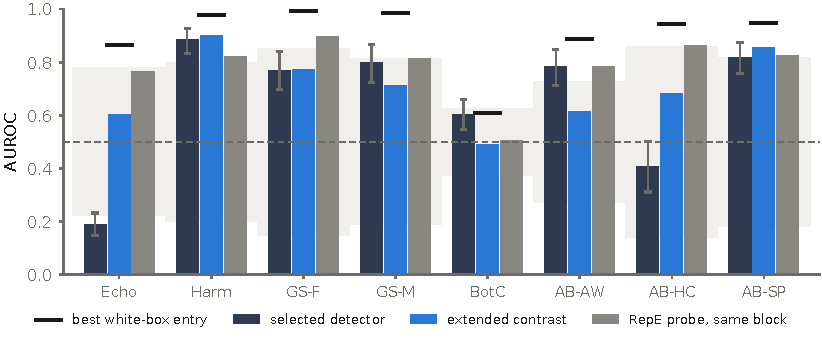
\includegraphics[width=0.9\linewidth]{fig_aletheia.pdf}
\caption{Aletheia's Quest per dataset: the selected detector with its interval, the extended contrast
and the RepE probe, the random band (grey) and the best white-box entry (bar).}
\label{fig:aletheia}
\end{figure}

\FloatBarrier
\section{The 150-question extension}
\label{app:qbank}

The pre-registration, the question grid and the drivers are in the repository. The 120 new questions were
written in one pass by an AI assistant (Claude) under a fixed prompt, frozen with the pre-registration
before any rollout was generated; prompt and raw output are archived with it. \Cref{tab:qbank-tests}
gives the tests, \cref{tab:qbank-families} the five-dataset mean of the extended contrast built from each
question family and the change from leaving that family out of the pooled bank, and
\cref{tab:qbank-confirm} the single confirmation read at every layer. The decision rule chose the bank by
the selected detector's five-dataset mean on development data, with ties within 0.005 going to the larger
bank; the four candidates lay within \V{qb-decision-spread}.

\begin{table}[h]
\centering
\footnotesize
\caption{The pre-registered tests of the question extension (Llama, layer 40).}
\label{tab:qbank-tests}
\resizebox{\linewidth}{!}{% Generated by make_arxiv_assets.py from results/question_bank/llama/verdict.csv
\begin{tabular}{@{}l >{\raggedright\arraybackslash}p{5.6cm} l@{}}
\toprule
Pre-registered test & Statistic & Result \\
\midrule
Variety beats count (extended contrast) & 30 originals + 30 monotone five-dataset mean 0.9044 vs 200 draws of 30 originals + 30 random diverse (median 0.8901), $p$ = 1.00 (Holm) & fails \\
Variety beats count (selected detector) & 30 originals + 30 monotone five-dataset mean 0.9097 vs 200 draws of 30 originals + 30 random diverse (median 0.9103), $p$ = 1.00 (Holm) & fails \\
Monotone additions behave like the originals & the monotone 30 0.9048 in [0.8296, 0.9114] of random 30 of 150; paired CI vs the original 30 [$-$0.0003, 0.0120] within $\pm$0.03 & passes \\
Pooling all 150 beats the best single family & all 150 0.8809 minus original knowledge family 0.9107 = $-$0.0298, CI [$-$0.0394, $-$0.0199], $p$ = 1.00 (Holm) & fails \\
Covariance-weighted cosine predicts transfer better than plain cosine & $R^2$ with the target's covariance 0.675 vs plain cosine 0.405; difference 0.269 CI [0.139, 0.365], $p < 0.001$ (Holm) & passes \\
More questions help on HP-KR's identical text (exploratory) & 0.7392 vs 0.7213, CI [0.0014, 0.0340] & passes \\
\bottomrule
\end{tabular}
}
\end{table}

\begin{table}[h]
\centering
\footnotesize
\caption{The extended contrast built from each question family, five-dataset mean at layer 40.}
\label{tab:qbank-families}
% Generated by make_arxiv_assets.py from results/question_bank/llama/spectrum_pooled_vs_family_L40.csv
\begin{tabular}{@{}l r c c@{}}
\toprule
Question family & Questions & \shortstack{Five-dataset\\mean AUROC} & \shortstack{Leaving it out:\\change vs pooled} \\
\midrule
Original: knowledge & 10 & 0.911 & $-$0.008 \\
Denial of knowledge & 15 & 0.907 & $-$0.014 \\
Monotone (new, same form) & 30 & 0.905 & $-$0.009 \\
Quality (false assertion) & 15 & 0.889 & $-$0.003 \\
Original: sycophancy & 10 & 0.874 & $-$0.000 \\
Original: disclosure & 10 & 0.872 & $-$0.002 \\
Relation (evasion) & 15 & 0.859 & $+$0.002 \\
Manner (equivocation) & 15 & 0.810 & $+$0.005 \\
Quantity (omission) & 15 & 0.800 & $+$0.008 \\
Sincere ignorance & 15 & 0.771 & $+$0.014 \\
Pooled, all 150 & 150 & 0.881 &  \\
\bottomrule
\end{tabular}

\end{table}

\begin{table}[h]
\centering
\footnotesize
\caption{The confirmation read: the 150-question bank against the 30-question bank, paired.}
\label{tab:qbank-confirm}
\resizebox{\linewidth}{!}{% Generated by make_arxiv_assets.py from results/question_bank/llama/confirm.csv
\begin{tabular}{@{}l l l c c c@{}}
\toprule
Layer & Set & Direction & 150 questions & 30 questions & Difference [95\%] \\
\midrule
20 & AISI held out & extended contrast & 0.974 & 0.971 & $+$0.003 [$+$0.000, $+$0.006] \\
20 & AISI held out & selected detector & 0.963 & 0.948 & $+$0.015 [$+$0.011, $+$0.019] \\
20 & Gender-Secret & extended contrast & 0.513 & 0.505 & $+$0.009 [$-$0.013, $+$0.031] \\
20 & Gender-Secret & selected detector & 0.526 & 0.532 & $-$0.005 [$-$0.021, $+$0.011] \\
36 & Gender-Secret & extended contrast & 0.444 & 0.409 & $+$0.035 [$+$0.002, $+$0.068] \\
36 & Gender-Secret & selected detector & 0.751 & 0.761 & $-$0.010 [$-$0.022, $+$0.003] \\
40 & AISI held out & extended contrast & 0.980 & 0.977 & $+$0.003 [$+$0.001, $+$0.005] \\
40 & AISI held out & selected detector & 0.966 & 0.960 & $+$0.006 [$+$0.004, $+$0.009] \\
40 & Gender-Secret & extended contrast & 0.491 & 0.467 & $+$0.024 [$-$0.005, $+$0.056] \\
40 & Gender-Secret & selected detector & 0.778 & 0.802 & $-$0.024 [$-$0.037, $-$0.010] \\
44 & AISI held out & extended contrast & 0.980 & 0.977 & $+$0.002 [$+$0.001, $+$0.004] \\
44 & AISI held out & selected detector & 0.965 & 0.961 & $+$0.004 [$+$0.003, $+$0.006] \\
44 & Gender-Secret & extended contrast & 0.605 & 0.541 & $+$0.064 [$+$0.041, $+$0.090] \\
44 & Gender-Secret & selected detector & 0.808 & 0.807 & $+$0.001 [$-$0.010, $+$0.013] \\
\bottomrule
\end{tabular}
}
\end{table}

\FloatBarrier
\section{Side results}
\label{app:side}

Four further studies on Llama bear on the method and are reported in the repository; their figures are
quoted from those reports. Attention probes trained on 76 per-token persona coordinates transfer worse
than the fixed reads at every layer (best trained arm 0.849 against 0.928 for the knowledge-denial
contrast's top-decile read at layer 40): learning the readout costs transfer. On the five-dataset mean AUROC,
averaging the zero-shot score over all 16 layers falls below layer~40 for every zero-shot direction (only
the supervised base probe gains, from 0.778 to 0.807); the average beats a randomly chosen layer on average
but neither layer~40 nor the best layer: a hedge, not a gain. A knowledge
follow-up question (``Did you actually know the answer?'') read at its prefilled ``No'' adds nothing over
the response read, and the sign of every direction there follows the prefilled word. Finally, the
covariance-weighted alignment of \citet{ying2026truthfulness} fits the transfer matrix ($R^2$ 0.82 for
the raw probe at layer 40, against 0.19 for the plain cosine), but the point-biserial correlation of a
detector's scores with the labels fits better (0.93): with the test set's pooled covariance and a
near-perfect own probe the alignment reduces to the detector's own effect size, which is the caveat
attached to the extension's fourth test. The same analysis shows that \hpkr's own probe plus the
knowledge-denial contrast beats the own probe at all 16 layers (0.949 to 0.978 at layer 40), so \hpkr{}
carries at least two separating directions.

\FloatBarrier
\section{Statistics and reproducibility}
\label{app:repro}

Intervals are percentile intervals over 1,000 stratified resamples of the test rows with one seed, the
same resamples for every detector, so differences are paired. Random bands are the 97.5th percentile of
the AUROCs of 1,000 random unit directions on the same rows and block, reseeded per study, which moves a
band by a few thousandths between files; the paper quotes the thesis's values. The block for each of
Llama's layers on the other models is the block at which the base probe reproduces the benchmark's
published Mean Probe (for layer~20), the middle block (for layer~40) and the blocks 5\% of the depth either
side; the sweep is the same 16 relative depths. Liars' Bench is read at the Hugging Face revision the
benchmark's Llama runs used, and the AISI rollouts at dataset revision 177a816. The generators are
\texttt{make\_arxiv\_assets.py}, which writes this paper's own numbers, tables and figures, and the thesis
generators it imports (\texttt{make\_numbers.py}, \texttt{make\_thesis\_assets.py},
\texttt{make\_xmodel\_assets.py}). The persona bank, the knowledge direction's questions, the
pre-registrations and every result file the generators read are at \repourl.


\end{document}
